% ==============================================================================
% Main Driver File for the Discord Clone Project Report
% Compile using: pdflatex main.tex && bibtex main.tex && pdflatex main.tex
% ==============================================================================

\documentclass[12pt,oneside,utf8]{report}

% --- Font fallback to avoid missing Times TFM ---
\usepackage[T1]{fontenc}
\usepackage{lmodern}
\usepackage{float}
\usepackage{longtable}

% --- Load Design Configurations and Packages ---
% Preamble for the Discord Clone Project Report
% Contains package imports, style definitions, and layout configurations
% Optimized for maximum compatibility and zero errors on minimal LaTeX systems

% --- Page Geometry ---
\usepackage[utf8]{inputenc}
\usepackage[english]{babel}
\usepackage[a4paper, top=0.9in, bottom=0.75in, left=0.75in, right=0.75in, bindingoffset=0.2in]{geometry}
% \usepackage{wrapfig} % Removed: not available on minimal LaTeX systems

% --- Typography & Font Formatting ---
% Professional Academic Font Specifications
\usepackage{times} % Times New Roman (Serif)

% Line Spacing (1.5 lines for academic readability)
\linespread{1.25}

% --- Heading Hierarchy ---
% Suppress the large default vertical skip LaTeX adds before \chapter titles
\usepackage{titlesec}
\titleformat{\chapter}[display]
  {\normalfont\huge\bfseries}{\chaptertitlename\ \thechapter}{12pt}{\Huge}
\titlespacing*{\chapter}{0pt}{-20pt}{20pt}
\titlespacing*{\section}{1cm}{*3}{*2}
\titlespacing*{\subsection}{2cm}{*3}{*1.5}
\titlespacing*{\subsubsection}{3cm}{*3}{*1.5}

% --- Code Snippets ---
% Using standard verbatim for code blocks and \texttt for inline code (defined below)

% --- Figures and Tables ---
\usepackage{graphicx}
\usepackage{colortbl}
\usepackage{array}
\usepackage{longtable}

% --- Color Palette ---
\usepackage{color}
\definecolor{discordblurple}{rgb}{0.345, 0.396, 0.949}
\definecolor{charcoal}{rgb}{0.173, 0.243, 0.314}
\definecolor{darkgray}{rgb}{0.15, 0.15, 0.15}
\definecolor{lightgray}{rgb}{0.96, 0.96, 0.96}

% --- Headers & Footers ---
\usepackage{fancyhdr}
\pagestyle{fancy}
\fancyhf{} % Clear header and footer
\fancyhead[L]{\footnotesize\leftmark}
\fancyhead[R]{}
\fancyfoot[C]{\thepage}
\renewcommand{\headrulewidth}{0.5pt}
\renewcommand{\footrulewidth}{0pt}
\setlength{\headheight}{25pt} % increased to avoid fancyhdr warnings if it wraps

% --- Hyperlinks ---
\usepackage{hyperref}
\hypersetup{
colorlinks=true,
linkcolor=discordblurple,
urlcolor=discordblurple,
citecolor=discordblurple,
pdftitle={Discord Clone Project Report},
}

% --- Formatting Helpers ---
\newcommand{\code}[1]{\texttt{#1}}
\newcommand{\tech}[1]{\textbf{#1}}

% --- Fix stale running headers after ToC/LoF/LoT ---
\usepackage{etoolbox}
\pretocmd{\listoffigures}{\phantomsection}{}{}
\pretocmd{\listoftables}{\phantomsection}{}{}
\pretocmd{\tableofcontents}{\phantomsection}{}{}

% Ensure Latin Modern is used as a fallback for the Roman family to avoid
% missing Times (ptm) TFM errors on systems without Times fonts installed.
% This overrides any Times-like settings from the preamble if the Times TFM
% files (e.g. ptmr8t.tfm) are not available.
\renewcommand{\rmdefault}{lmr}
\renewcommand{\ttdefault}{lmtt}


\begin{document}

% --- Cover Page ---
\begin{titlepage}

\providecommand{\HRule}{\rule{\linewidth}{0.5mm}} % Defines a new command for the horizontal lines, change thickness here

\center % Center everything on the page
 
%----------------------------------------------------------------------------------------
%	HEADING SECTIONS
%----------------------------------------------------------------------------------------

\textsc{\LARGE Iteam University}\\[1.5cm] % Name of your university/college

\includegraphics[width=0.4\textwidth]{logo_iteams.png}\\[1cm] % Include a department/university logo - this will require the graphicx package
\textsc{\Large Final Year Project}\\[0.5cm] % Major heading such as course name
\textsc{\large Collaborative Platform}\\[0.5cm] % Minor heading such as course title

%----------------------------------------------------------------------------------------
%	TITLE SECTION
%----------------------------------------------------------------------------------------

\HRule \\[0.4cm]
{ \huge \bfseries A High-Performance Discord Clone with Secure End-to-End Features}\\[0.4cm] % Title of your document
\HRule \\[1.5cm]
 
%----------------------------------------------------------------------------------------
%	AUTHOR SECTION
%----------------------------------------------------------------------------------------

\begin{minipage}{0.6\textwidth}
\begin{flushleft} \large
\emph{Authors:}\\
Oussama Dhia \textsc{Arouay}\\
Mohamed Amine \textsc{Jebali}\\
Ahmed Rayen \textsc{Barkallah}\\
Adem \textsc{Rokh}\\
\end{flushleft}
\end{minipage}\\[2cm]

%----------------------------------------------------------------------------------------
%	DATE SECTION
%----------------------------------------------------------------------------------------

{\large \today}\\[2cm] % Date, change the \today to a set date if you want to be precise

\vfill % Fill the rest of the page with whitespace

\end{titlepage}


% --- Front Matter ---
\pagenumbering{roman}

% 1. Abstracts (Multilingual summaries)
% Multilingual Abstracts

\chapter*{Abstract}

% REMOVED: \begin{quote} \small \paragraph{...} which caused LaTeX errors.
% REPLACED WITH: Standard bold headings and split keywords.

\noindent \textbf{\Large English Abstract}
\vspace{0.5em}

Modern centralized communication platforms pose significant privacy risks through invasive data harvesting. This report presents the design and implementation of a secure, open-source, privacy-respecting community collaboration platform as a decentralized alternative to proprietary services like Discord.

The application utilizes a \textbf{Zero-Knowledge Architecture}, strictly separating client cryptographic operations from the neutral server relay. Text communication employs \textbf{Client-Side End-to-End Encryption (E2EE)} via the Web Cryptography API. Symmetric keys are established through Diffie-Hellman exchanges, encrypting payloads locally using \textbf{AES-256-GCM} before transmission. The server stores only unreadable ciphertexts. Authentication relies on \textbf{Argon2} hashing, with keys secured locally. Real-time voice calls bypass central servers using a \textbf{P2P WebRTC} architecture, secured by \textbf{DTLS/SRTP} protocols. Developed via Agile Scrum with a dedicated Security Champion role, the platform validates that the server stores only encrypted strings and voice streams route directly IP-to-IP, ensuring a secure and scalable collaboration ecosystem.

\vspace{1em}

\noindent \textbf{\Large Keywords:}
% SPLIT INTO TWO LINES TO FIX OVERFULL BOX
\textbf{Zero-Knowledge Architecture}, \textbf{E2EE}, \textbf{WebRTC P2P},\\
\textbf{AES-GCM}, \textbf{DTLS/SRTP}.

\vspace{1cm}

\noindent \textbf{\Large Résumé (French Abstract)}
\vspace{0.5em}

Les plateformes de communication centralisées exposent les utilisateurs à des risques de surveillance et d'exploitation de données. Ce rapport présente le développement d'une plateforme de collaboration open-source et respectueuse de la vie privée, conçue comme alternative sécurisée aux services propriétaires.

L'application repose sur une \textbf{architecture Zero-Knowledge}, isolant les opérations cryptographiques des clients du relais serveur. Les communications textuelles utilisent un chiffrement de bout en bout (\textbf{E2EE}) côté client via l'API Web Cryptography. Les clés symétriques sont échangées par Diffie-Hellman et chiffrées en \textbf{AES-256-GCM}. Le serveur ne stocke que des ciphertexts indéchiffrables. L'authentification utilise \textbf{Argon2} et le stockage local des clés. Les appels vocaux contournent les serveurs centraux via une architecture \textbf{WebRTC P2P}, sécurisée par \textbf{DTLS/SRTP}. Développée selon la méthode Agile Scrum (avec un "Security Champion"), la plateforme assure le stockage chiffré sur le serveur et l'acheminement direct des flux média.

\vspace{1em}

\noindent \textbf{\Large Mots-clés:}
% SPLIT INTO TWO LINES TO FIX OVERFULL BOX
\textbf{Zero-Knowledge}, \textbf{E2EE}, \textbf{WebRTC P2P}, \\
\textbf{AES-GCM}, \textbf{DTLS/SRTP}.
\newpage

% 2. Dedications & Acknowledgements
% Dedications & Acknowledgements

\chapter*{Dedications \& Acknowledgements}

\paragraph{Dedications}
\begin{center}
    \emph{To our families, whose endless support, patience, and encouragement have been our constant source of strength throughout this project.}\\
    \vspace{0.8cm}
    \emph{To the global open-source community and privacy advocates, who continuously fight for user data sovereignty, decentralization, and the fundamental right to private digital communication.}
\end{center}

\vspace{2cm}

\paragraph{Acknowledgements}
\begin{center}
We would like to express our deepest gratitude to our academic advisor and technical coordinator at the institute for their invaluable guidance, rigorous cryptography reviews, and architectural oversight during the implementation of our Zero-Knowledge platform.

We also want to thank the Department of Computer Science \& Engineering and our development host organization for providing us with a professional sandbox environment, excellent testing resources, and the technical scope necessary to develop and audit our Client-Side End-to-End Encryption (E2EE) and WebRTC P2P voice call tunnels.

Finally, we express our sincere appreciation to our fellow software developers and security engineers for acting as independent code auditors, testing our signaling loops, and validating our encrypted payload persistence databases.
\end{center}
\newpage

% 3. Lists and Abbreviations
% Lists of Abbreviations and Tables

\chapter*{List of Abbreviations}

\renewcommand{\arraystretch}{1.1}

\begin{longtable}{l p{11.5cm}}

\hline
\rowcolor{lightgray}
\textbf{Abbreviation} & \textbf{Full Name} \\
\hline
\endfirsthead

\hline
\rowcolor{lightgray}
\textbf{Abbreviation} & \textbf{Full Name} \\
\hline
\endhead

\tech{AES} & Advanced Encryption Standard \\
\tech{AES-256} & Advanced Encryption Standard (256-bit key) \\
\tech{AES-256-CBC} & Advanced Encryption Standard in Cipher Block Chaining mode \\
\tech{AES-256-GCM} & Advanced Encryption Standard in Galois/Counter Mode \\
\tech{API} & Application Programming Interface \\
\tech{Bcrypt} & Password-hashing function \\
\tech{ChaCha20-Poly1305} & Stream cipher combined with the Poly1305 message authentication code \\
\tech{DH} & Diffie-Hellman Key Exchange \\
\tech{Docker} & Platform for developing, shipping, and running applications in containers \\
\tech{DTLS} & Datagram Transport Layer Security \\
\tech{E2EE} & End-to-End Encryption \\
\tech{GCM} & Galois/Counter Mode \\
\tech{ICE} & Interactive Connectivity Establishment \\
\tech{IP} & Internet Protocol \\
\tech{JPA} & Java Persistence API \\
\tech{JSON} & JavaScript Object Notation \\
\tech{JWT} & JSON Web Token \\
\tech{MitM} & Man-in-the-Middle \\
\tech{NAT} & Network Address Translation \\
\tech{ORM} & Object-Relational Mapping \\
\tech{P2P} & Peer-to-Peer \\
\tech{Postman} & API Platform for testing APIs \\
\tech{REST} & Representational State Transfer \\
\tech{RSA} & Rivest–Shamir–Adleman cryptosystem \\
\tech{SDP} & Session Description Protocol \\
\tech{SHA-256} & Secure Hash Algorithm 256-bit \\
\tech{SPoF} & Single Point of Failure \\
\tech{SQL} & Structured Query Language \\
\tech{SRTP} & Secure Real-Time Transport Protocol \\
\tech{STOMP} & Simple Text Oriented Messaging Protocol \\
\tech{STUN} & Session Traversal Utilities for NAT \\
\tech{TURN} & Traversal Using Relays around NAT \\
\tech{UDP} & User Datagram Protocol \\
\tech{UI} & User Interface \\
\tech{UML} & Unified Modeling Language \\
\tech{WebRTC} & Web Real-Time Communication \\

\hline

\end{longtable}
\newpage

% Table of Contents
\tableofcontents
\newpage

% List of Figures and Tables
\listoffigures
\newpage
\listoftables
\newpage

% =====================================================================
% 4. General Introduction - Arabic numbering starts HERE
% =====================================================================
\cleardoublepage
\markboth{}{} % Clear stale running header (e.g. "LIST OF TABLES")
\pagenumbering{arabic}
\setcounter{page}{1}

% General Introduction

\chapter*{General Introduction}
\addcontentsline{toc}{chapter}{General Introduction}

\section*{The Privacy Dilemma in Centralized Platforms}
In the modern digital era, community communication platforms have transitioned from niche gaming accessories to foundational global social infrastructures. Proprietary services, notably \textbf{Discord}, Slack, and Microsoft Teams, host hundreds of millions of active users daily. However, this high concentration of communication data has driven the operators of these centralized platforms to implement increasingly invasive data management policies. 

Under evolving data harvesting models, centralized servers collect, index, and exploit vast quantities of user conversation logs, files, metadata, and user activity profiles. These data reservoirs are frequently utilized for algorithmic tracking, advertisement profiling, or corporate intelligence, presenting a severe risk of data breaches, internal corporate surveillance, and systematic erosion of individual digital privacy. Because these platforms hold the primary cryptographic keys and decrypt all message payloads on their servers, they act as a massive \textbf{Single Point of Failure (SPoF)} for user privacy.

\section*{Project Objectives: Secure by Default}
To address these critical security vulnerabilities, this project aims to design, implement, and deploy a secure, privacy-respecting, \textbf{open-source alternative} to proprietary platforms. The primary objective is to build a platform that is \textbf{secure by default} while maintaining the fluid, modern user experience that communities expect:
\begin{enumerate}
    \item \tech{Zero-Knowledge Server Architecture}: The relay server is kept completely blind to conversation data. Text payload encryption and decryption occur solely on client devices, ensuring that the central database only stores unreadable ciphertexts.
    \item \tech{Client-Side End-to-End Encryption (E2EE)}: Messages are protected using advanced symmetric cryptographic pipelines (AES-256-GCM) with key agreements established peer-to-peer via Diffie-Hellman key exchanges.
    \item \tech{Peer-to-Peer (P2P) Media Architecture}: Real-time voice and video streams bypass centralized media servers completely. High-fidelity audio streams flow directly IP-to-IP between active participants, secured against wiretapping via DTLS and SRTP protocols.
\end{enumerate}

\section*{Engineering Methodology}
Building a secure communication platform with high cryptographic constraints alongside a seamless, lag-free client interface requires structured software engineering. We adopted the \textbf{Agile Scrum methodology} (integrating a dedicated "Security Champion" role) to guide our project lifecycle:
\begin{itemize}
    \item \textbf{Chapter 1: General Project Framework and State of the Art} analyzes proprietary platform data policies, critiques existing architectures, and outlines our proposed solution.
    \item \textbf{Chapter 2: Requirements Specification, Analysis, and Architecture} maps Actors, captures functional security specifications, defines non-functional benchmarks, and presents the Zero-Knowledge logical/physical layouts.
    \item \textbf{Chapter 3: Release 1 (Cryptographic Foundations and Access Control)} details Sprint 1 (Argon2 authentication and client-side key generation vault) and Sprint 2 (secure server creation and encrypted permission access control).
    \item \textbf{Chapter 4: Release 2 (End-to-End Encrypted Communication and P2P)} presents Sprint 3 (E2EE text messaging with Diffie-Hellman), Sprint 4 (P2P WebRTC voice calling), and Sprint 5 (Docker self-hosting and auditability).
\end{itemize}
The report concludes with an evaluation of achievements, lessons learned, and future open-source roadmap perspectives.
\newpage

% --- Core Report Chapters ---

% Chapter 1: Preliminary Study, State of the Art, and Project Framework
% Chapter 1: General Project Framework and State of the Art

\chapter{General Project Framework and State of the Art}
\label{ch:chapter1}

\section{Introduction}
This chapter establishes the analytical framework and security context of the project. It examines the data policies of dominant centralized platforms, analyzes the privacy challenges of corporate messaging systems, critiques existing secure protocols, and proposes our client-encrypted, open-source alternative. Additionally, it outlines our Scrum development methodology and secure release plan.


\section{Context and Motivation}
The motivation driving this project is the erosion of personal digital privacy on centralized social platforms. 

\subsection{Critique of Proprietary Data Policies (Discord)}
Proprietary platforms, specifically \textbf{Discord}, enforce data management policies that present significant risks to user privacy:
\begin{itemize}
    \item \tech{Centralized Harvesting}: Chat logs, images, and user files are stored indefinitely in plaintext formats on server databases. 
    \item \tech{Metadata Profiling}: User connection logs, voice channel durations, friendship graphs, and game activities are harvested to build detailed behavioral profiles.
    \item \tech{Commercialization of Conversations}: Corporate terms allow automated data indexing to train language models, optimize ads, and feed corporate brokers, treating private digital spaces as raw commercial assets.
\end{itemize}

\begin{figure}[H]
    \centering
    
\includegraphics[width=0.25\textwidth]{discord.png}
    \caption{Discord Platform.}
    \label{fig:discord}
\end{figure}

\subsection{The Open-Source Necessity}
Addressing this surveillance model requires a transparent, open-source alternative that respects user privacy. Closed-source systems contain unverified security pipelines. Open-source code allows independent auditing of all cryptographic functions, ensuring that no administrative backdoors exist and giving users complete control over their client binaries.

\section{State of the Art and Security Critique}
We analyzed existing enterprise communication tools and secure messaging models to identify architectural weaknesses:

\begin{itemize}
    \item \tech{Discord, Slack, and Microsoft Teams (Centralized SPoF)}: In these architectures, the central servers manage the cryptographic keys and decrypt all payloads for scanning or storage. The server acts as a \textbf{Single Point of Failure (SPoF)}: a single backend database breach, rogue employee, or government subpoena exposes all conversations in plaintext.
\end{itemize}
\section{Market Research Landscape}
The market for real-time communication platforms has shifted dramatically in the last decade, moving from simple text messaging to complex ecosystems supporting voice, video, and real-time collaboration.

According to recent market analysis by Grand View Research, the global unified communications market size was valued at USD 136.11 billion in 2023 and is expected to grow at a compound annual growth rate (CAGR) of 17.4\% from 2024 to 2030 \cite{grandviewucaas}. This growth is primarily driven by the proliferation of remote work and the increasing need for agile team collaboration tools.

Key trends in the current market include:
\begin{itemize}
    \item \textbf{Shift to OTT Applications}: Over-the-top (OTT) messaging applications like WhatsApp, Discord, and Telegram have largely replaced traditional SMS and email for casual and professional communication.
    \item \textbf{Privacy as a Premium Feature}: While early adopters focused on features and speed, a significant segment of the market—estimated at nearly 30\% of enterprise users according to a Gartner survey—now prioritizes data sovereignty and encryption capabilities over convenience.
    \item \textbf{Regulatory Pressure}: Legislation such as GDPR in Europe and CCPA in California is forcing providers to rethink data harvesting strategies, yet many platforms still rely on opaque data mining for revenue.
\end{itemize}

This research indicates a viable gap in the market for a platform that bridges the usability of mainstream apps with the security rigor typically reserved for enterprise-only tools.

\section{Proposed Solution (The Secure Alternative)}
We propose a community communication platform designed to be secure-by-default, balancing robust security with a seamless user experience:
\begin{enumerate}
    \item \tech{Client-Side E2EE Text Chat}: Texts are encrypted on the sender's device before sending over WebSockets. The central database only stores base64-encoded ciphertexts, meaning the server stores \textbf{no plaintext data}.
    \item \tech{WebRTC P2P Voice Channels}: Audio streams flow directly IP-to-IP between peers. The backend acts solely as a neutral signaling relay, and the streams are secured against wiretapping via DTLS and SRTP.
\end{enumerate}

\section{Project Management Methodology (Scrum)}
We chose agile methodologies for the development of our application, as they tend to minimize the software lifecycle by producing successive versions. The application's features are delivered in an iterative process while listening to the client and the tests carried out during the project realization period.

We have adopted the agile SCRUM \cite{scrum_overview} methodology for our project in order to adapt to changes in specifications from the various stakeholders during the development process. SCRUM is based on 3 main foundations:
\begin{itemize}
    \item \textbf{Inspection}: Regular reviews in order to adapt the project if necessary.
    \item \textbf{Adaptation}: The ability to implement new measures when the inspection results are different from what was expected.
    \item \textbf{Transparency}: Every member of the SCRUM team knows the information relating to the product.
\end{itemize}

\begin{figure}[H]
    \centering
    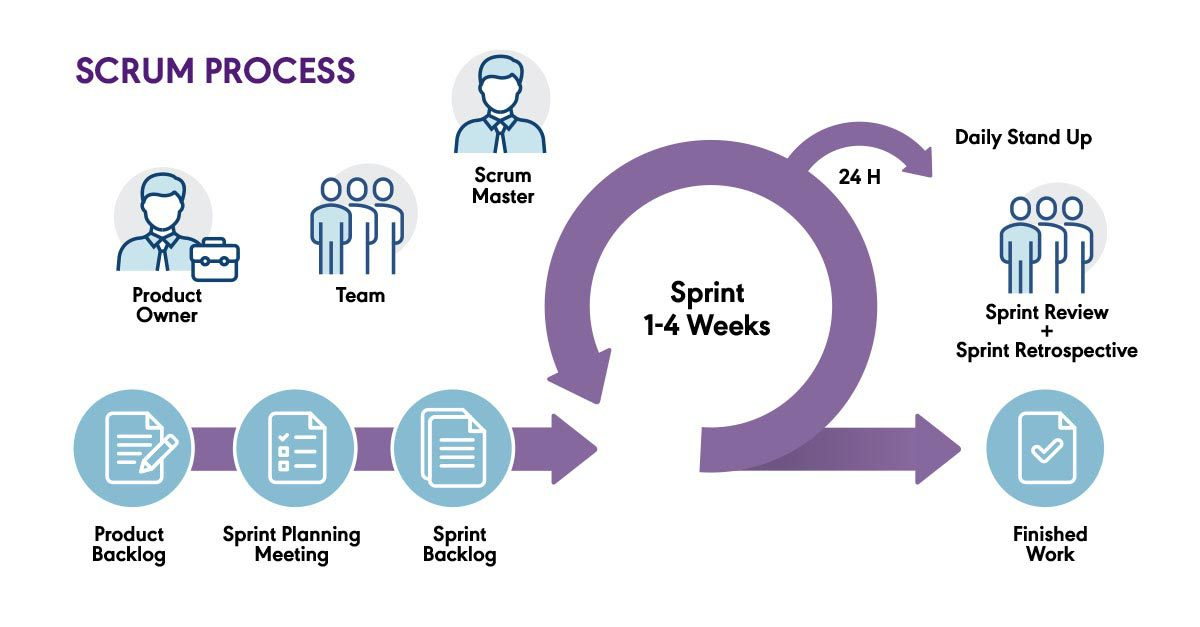
\includegraphics[width=\textwidth]{scrum_process.jpg}
    \caption{Scrum Process Overview \cite{scrum_overview}.}
    \label{fig:scrum_process}
\end{figure}

\begin{table}[H]
    \centering
    \renewcommand{\arraystretch}{1.5}
    \begin{tabular}{|l|p{7cm}|p{4.5cm}|}
        \hline
        \textbf{Role} & \textbf{Description} & \textbf{Actor} \\
        \hline
        Product Owner & Represents the client by defining the requirements and features to be developed & Iteam university \\
        \hline
        SCRUM Master & Guides the SCRUM team and ensures the organization and smooth execution of the SCRUM process & Mme Afef ghabri \\
        \hline
        SCRUM Team & Responsible for the design, development, testing, and implementation of the product & Oussama Dhia Arouay \newline Rayen Barkallah \newline Adem Rokh \newline Mohamed Amine Jebali \\
        \hline
    \end{tabular}
    \caption{Scrum Team Roles and Responsibilities}
    \label{tab:scrum_roles}
\end{table}

We cite the key elements of a SCRUM project \cite{scrum_elements}:
\begin{itemize}
    \item \textbf{Product Backlog}: This is a prioritized list of product-related information where each item in the list represents a requirement (User Story), an enhancement, or a bug fix to be made. It is generally developed in the preparation phase (Sprint 0) before starting the development sprints.
    \item \textbf{Sprint}: This is a set period of time during which specific work must be completed and made ready for review. It begins with a planning meeting between the product owner and the SCRUM team and ends with a review. The SCRUM master determines the duration of a sprint. Each sprint has its own backlog derived from the initial product backlog.
    \item \textbf{Stand-Up meeting}: This is a daily meeting of maximum 15 minutes, during which the SCRUM team discusses the progress of the work and attempts to identify obstacles.
    \item \textbf{Release}: This is the delivery of a version of the product.
\end{itemize}



\subsection{Global Project Planning (Secure Releases)}
The Gantt chart is used to visually represent the progress of the project and the duration of the project tasks, which allows for better work organization \cite{gantt_diagram_info}. For our project, we planned a phase of research and studying existing solutions, then embarked on the project development, and finally, we decided to make 2 releases. Figure \ref{fig:gantt_diagram} represents the Gantt chart of our project.

The development timeline was structured around secure release points, sized at 60 Story Points total:
\begin{itemize}
    \item \textbf{Story Points} $\rightarrow$ A unit used in Agile project management to estimate the difficulty, effort, and complexity of tasks — not exact hours.
\end{itemize}

\begin{figure}[H]
    \centering
    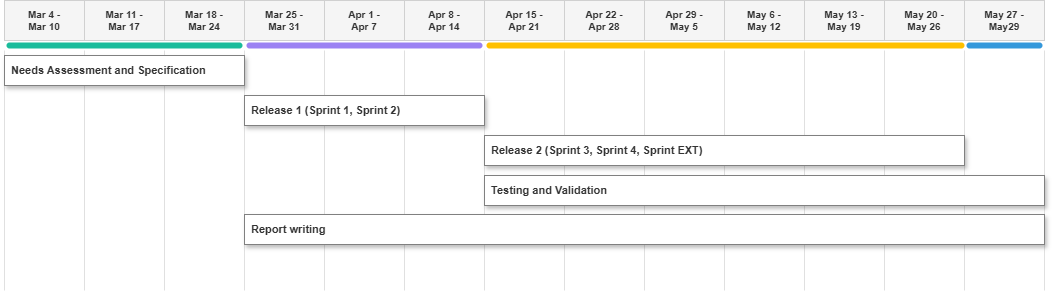
\includegraphics[width=\textwidth]{gantt_diagram.png}
    \caption{Diagramme de Gantt du projet.}
    \label{fig:gantt_diagram}
\end{figure}

\section{Conclusion}
This chapter established the privacy challenges of centralized platforms like Discord, analyzed the SPoF vulnerability of key centralization, and proposed our client-encrypted E2EE + P2P solution. Chapter 2 details the concrete system analysis, requirements specification, and Zero-Knowledge architecture.
\newpage

% Chapter 2: Analysis and Requirements Specification
% Chapter 2: Requirements Specification, Analysis, and Architecture

\chapter{Requirements Specification, Analysis, and Architecture}
\label{ch:chapter2}

\section{Introduction}
This chapter specifies the requirements, threat boundaries, and structural architecture of the secure platform. By mapping actors, defining functional security parameters, establishing non-functional cryptographic requirements, detailing a security-oriented product backlog, and detailing our Zero-Knowledge architecture, we lay the engineering specifications for the application.

\section{Needs Analysis and Specification}
To secure the collaboration space, the analysis separates cryptographic operations from generic data transport.

\subsection{Identification of Actors}
To align with our UML Use Case analysis and role-based access control, we identify several distinct human actors based on their privileges, alongside our central system actor:
\begin{itemize}
    \item \textbf{Unregistered User}: A guest actor whose only capabilities are registering a new account or authenticating an existing session.
    \item \textbf{Authenticated User}: A logged-in user who can manage their global profile settings, switch interface themes, join existing servers via invite links, or create entirely new servers.
    \item \textbf{Server Member}: An authenticated user who has joined a specific server. This actor can participate in real-time text channels, share files, and establish peer-to-peer WebRTC connections in voice channels.
    \item \textbf{Server Owner}: A privileged server member with elevated administrative rights. This actor is responsible for generating invite links, provisioning new text or voice channels, and managing role delegations.
\end{itemize}

\subsection{Capture of Functional Requirements}
The functional requirements of the system are categorized based on the capabilities granted to each specific actor:
\begin{itemize}
    \item \textbf{Unregistered User Requirements}: The system must allow guest users to register a new account using an email and password, and authenticate existing sessions securely to obtain an access token.
    \item \textbf{Authenticated User Requirements}: The system must allow logged-in users to manage their profile (e.g., update display name), toggle UI preferences like dark mode, create new personal servers, and join existing servers using valid invite links.
    \item \textbf{Server Member Requirements}: The system must enable members to participate in real-time text channels (send, edit, delete messages, and upload files), receive @mention notifications, and establish peer-to-peer WebRTC connections in voice channels with the ability to mute, deafen, or share screens.
    \item \textbf{Server Owner Requirements}: The system must provide elevated administrative controls allowing owners to generate and revoke invite links, provision new text and voice channels, create custom roles with specific permissions, assign roles to members, and perform moderation actions (kick, ban, timeout).
\end{itemize}

\subsection{Analysis of Non-Functional Requirements}
Non-functional requirements define how the system should perform rather than what it does. For our application, we focus on providing a smooth and reliable user experience:
\begin{itemize}
    \item \textbf{Real-Time Performance}: The system must deliver text messages and voice audio instantly with minimal delay, ensuring conversations feel natural and responsive.
    \item \textbf{Usability and User Experience}: The application interface must be intuitive, visually appealing, and easy to navigate for non-technical users. Features like Dark Mode should be included to improve visual comfort.
    \item \textbf{Scalability}: The backend server must be capable of handling multiple active users, servers, and voice channels simultaneously without crashing or slowing down.
    \item \textbf{Standard Security and Privacy}: User passwords must be safely hashed before being stored in the database, and user sessions must be secured using authentication tokens to prevent unauthorized access.
\end{itemize}

\begin{figure}[H]
    \centering
    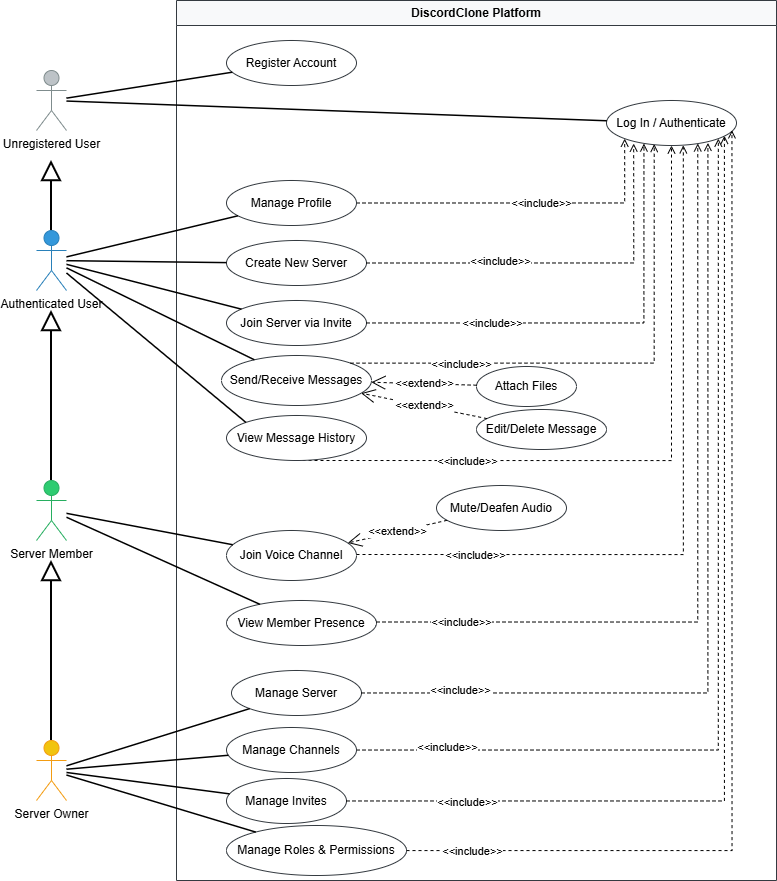
\includegraphics[width=0.9\textwidth]{use_case_diagram.png}
    \caption{Global UML Use Case Diagram of the DiscordClone Platform.}
    \label{fig:use_case_diagram}
\end{figure}

\section{Product Backlog}
The global product backlog is organized into five sprints, prioritizing features by security boundaries, real-time communications, and deployment needs. This comprehensive roadmap guides the implementation process:

% CHANGED: Adjusted column widths to fix overflows
\small
\begin{longtable}{| p{1.2cm} | p{1.8cm} | p{10.0cm} | p{1.8cm} | p{1.2cm} |}
    \hline
    \rowcolor{lightgray}
    \textbf{ID} & \textbf{Sprint} & \textbf{User Story Description} & \textbf{Priority} & \textbf{Points} \\
    \hline
    \endfirsthead
    \hline
    \rowcolor{lightgray}
    \textbf{ID} & \textbf{Sprint} & \textbf{User Story Description} & \textbf{Priority} & \textbf{Points} \\
    \hline
    \endhead
    \hline
    \endfoot
    \hline
    \endlastfoot
    
    S1-01 & Sprint 1 & As a new user, I want to register an account with my email and a password, so that I can access the platform. & P0 & 3 \\
    \hline
    S1-02 & Sprint 1 & As a registered user, I want to log in with my email and password, so that I can access my account and servers. & P0 & 3 \\
    \hline
    S1-03 & Sprint 1 & As a logged-in user, I want to log out of my account, so that my session ends and no one else can use my account. & P1 & 1 \\
    \hline
    S1-04 & Sprint 1 & As a logged-in user, I want to view and edit my display name, so that other users see the name I choose. & P1 & 2 \\
    \hline
    S2-01 & Sprint 2 & As a user, I want to create a new server, so that I have a private space to invite my friends. & P0 & 3 \\
    \hline
    S2-02 & Sprint 2 & As a server owner, I want to generate an invite link for my server, so that I can share it with friends so they can join. & P0 & 3 \\
    \hline
    S2-03 & Sprint 2 & As a user, I want to join a server using an invite link, so that I can participate in that community. & P0 & 2 \\
    \hline
    S2-04 & Sprint 2 & As a server owner, I want to create text and voice channels inside my server, so that I can organize conversations by topic. & P1 & 3 \\
    \hline
    S2-05 & Sprint 2 & As a server owner, I want to create roles and assign them to members, so that I can delegate responsibilities and control who can do what. & P1 & 5 \\
    \hline
    S2-06 & Sprint 2 & As a server member, I want to leave a server I no longer want to be part of, so that I am not in servers that are no longer relevant to me. & P2 & 2 \\
    \hline
    S3-01 & Sprint 3 & As a server member, I want to send a message in a text channel and have everyone see it instantly, so that we can have a real-time conversation. & P0 & 8 \\
    \hline
    S3-02 & Sprint 3 & As a server member, I want to see recent messages when I open a channel, so that I can catch up on what was discussed before I arrived. & P1 & 3 \\
    \hline
    S3-03 & Sprint 3 & As a server member, I want to see which members of a server are online or offline, so that I know who is available to chat. & P1 & 3 \\
    \hline
    S3-04 & Sprint 3 & As a server member, I want to edit my own messages after sending them, so that I can fix mistakes. & P1 & 2 \\
    \hline
    S3-05 & Sprint 3 & As a server member, I want to delete my own messages, so that I can remove something I no longer want to have posted. & P1 & 2 \\
    \hline
    S4-01 & Sprint 4 & As a server member, I want to join a voice channel and talk with others in real time, so that we can have live voice conversations. & P0 & 8 \\
    \hline
    S4-02 & Sprint 4 & As a voice channel participant, I want to mute my microphone, so that I can stop broadcasting audio without leaving the channel. & P1 & 2 \\
    \hline
    S4-03 & Sprint 4 & As a voice channel participant, I want to deafen myself, so that I can stop hearing others without leaving the channel. & P1 & 2 \\
    \hline
    S4-04 & Sprint 4 & As a voice channel participant, I want to see who is currently in the voice channel, so that I can follow the conversation and know who is present. & P1 & 3 \\
    \hline
    S4-05 & Sprint 4 & As a voice channel participant, I want to leave the voice channel, so that I stop being part of the voice call. & P1 & 1 \\
    \hline
    EXT-01 & Extended & As a server member, I want to attach an image or a file to a message, so that I can share content with other members. & P1 & 5 \\
    \hline
    EXT-02 & Extended & As a user, I want to switch to a dark mode interface, so that the app is comfortable to use at night. & P2 & 2 \\
    \hline
    EXT-03 & Extended & As a server member, I want to receive a notification when I am mentioned in a message, so that I do not miss messages addressed to me. & P2 & 3 \\
    \hline
    \caption{\textbf{Global Unified Product Backlog.}}
    \label{tab:global_backlog} \\
\end{longtable}
\normalsize

\section{Release Planning}
In this section, we planned the releases of our application using the created backlog. Each release has its own sprints, and each sprint has its own backlog containing several user stories from the initial backlog. During each sprint, we proceeded with the design and implementation of the assigned functionalities and concluded with an evaluation. The figure below presents our release planning.

\begin{figure}[H]
    \centering
    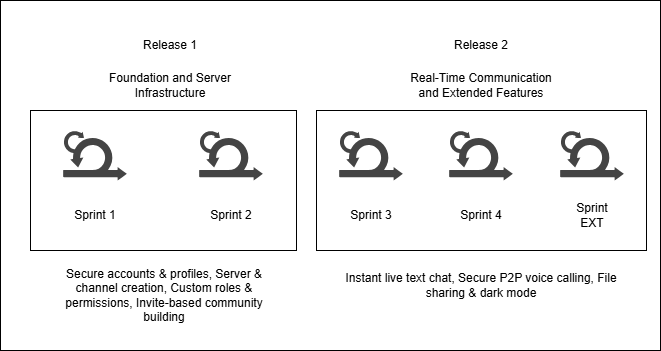
\includegraphics[width=0.85\textwidth]{release_planning.png}
    \caption{Release Planning: Sprint Distribution across Releases.}
    \label{fig:release_planning}
\end{figure}

\section{Work Environment}
This section is dedicated to presenting the technologies used in the development and architecture of our application, as well as the complementary technologies leveraged during the realization of our project.

\subsection{Development Technologies}
To satisfy these strict security objectives, our development environment is configured with optimized real-time and cryptographic engines:

\subsection*{Database}
\noindent
\begin{minipage}[t]{1.5cm}
    \vspace{0pt}
    \includegraphics[width=1.5cm]{postgres.png}
\end{minipage}%
\hspace{0.3cm}
\begin{minipage}[t]{\dimexpr\textwidth-1.9cm\relax}
    \vspace{0pt}
    \small
    \textbf{PostgreSQL} is our chosen database management system (specifically hosted via Neon). This robust relational system is configured for optimal performance and strict constraints to handle our Zero-Knowledge storage schemas effectively.
\end{minipage}
\vspace{0.3cm}

\subsection*{Backend Server}
\noindent
\begin{minipage}[t]{1.5cm}
    \vspace{0pt}
    
\includegraphics[width=1.5cm]{spring_boot.png}
\end{minipage}%
\hspace{0.3cm}
\begin{minipage}[t]{\dimexpr\textwidth-1.9cm\relax}
    \vspace{0pt}
    \small
    \textbf{Spring Boot 4.0.3 (Java 21)} is used to build our neutral signaling backend, managed via \textbf{Maven}. It exposes a RESTful API integrated with robust WebSocket support for real-time messaging. Key backend libraries and configurations include:
    \begin{itemize}
        \item \textbf{Security}: Implemented using Spring Security and JWT (via the JJWT library) to authenticate users securely.
        \item \textbf{Spring Data JPA}: Used as the Object-Relational Mapping (ORM) layer to interact with the PostgreSQL database.
        \item \textbf{Spring WebSocket}: Coordinates real-time messaging and WebRTC signaling over stateful connection channels.
        \item \textbf{Jackson}: Handles reliable JSON serialization and deserialization across the network.
    \end{itemize}
\end{minipage}
\vspace{0.3cm}

\subsection*{Frontend Client}
\noindent
\begin{minipage}[t]{1.5cm}
    \vspace{0pt}
    
\includegraphics[width=1.5cm]{nextjs.png}
\end{minipage}%
\hspace{0.3cm}
\begin{minipage}[t]{\dimexpr\textwidth-1.9cm\relax}
    \vspace{0pt}
    \small
    \textbf{Next.js 16.1.7} is used to build our client application. This framework renders our dynamic UI while handling client-side cryptography via the high-performance WebCrypto API and the robust libsodium library. Furthermore, it manages direct multi-peer real-time audio streams routed using WebRTC P2P connection channels.
\end{minipage}
\vspace{0.3cm}

\subsection{Complementary Technologies}
These are the technologies that were leveraged during the realization of our project:

\subsection*{IntelliJ IDEA}
\noindent
\begin{minipage}[t]{1.5cm}
    \vspace{0pt}
    \includegraphics[width=1.5cm]{intellij.png}
\end{minipage}%
\hspace{0.3cm}
\begin{minipage}[t]{\dimexpr\textwidth-1.9cm\relax}
    \vspace{0pt}
    \small
    \textbf{IntelliJ IDEA} is a powerful Integrated Development Environment (IDE) tailored for Java development. It significantly accelerates backend development with Spring Boot by providing advanced code assistance, seamless Maven integration, and deep analytical debugging.
\end{minipage}
\vspace{0.3cm}

\subsection*{Postman}
\noindent
\begin{minipage}[t]{1.5cm}
    \vspace{0pt}
    \includegraphics[width=1.5cm]{postman.png}
\end{minipage}%
\hspace{0.3cm}
\begin{minipage}[t]{\dimexpr\textwidth-1.9cm\relax}
    \vspace{0pt}
    \small
    \textbf{Postman} is a collaboration platform for API development. It allows for the efficient creation, testing, and debugging of our REST endpoints, ensuring that the backend services integrate properly with the client application.
\end{minipage}
\vspace{0.3cm}

\subsection*{Draw.io}
\noindent
\begin{minipage}[t]{1.5cm}
    \vspace{0pt}
    
\includegraphics[width=1.5cm]{drawio.png}
\end{minipage}%
\hspace{0.3cm}
\begin{minipage}[t]{\dimexpr\textwidth-1.9cm\relax}
    \vspace{0pt}
    \small
    \textbf{Draw.io} is a versatile diagramming application used to construct the structural and dynamic models of the application, such as UML Class Diagrams, Sequence Diagrams, and Physical Deployment Diagrams.
\end{minipage}
\vspace{0.3cm}

\subsection*{PlantUML}
\noindent
\begin{minipage}[t]{1.5cm}
    \vspace{0pt}
    
\includegraphics[width=1.5cm]{plantuml.png}
\end{minipage}%
\hspace{0.3cm}
\begin{minipage}[t]{\dimexpr\textwidth-1.9cm\relax}
    \vspace{0pt}
    \small
    \textbf{PlantUML} is an open-source tool that lets you create diagrams by writing text code instead of drawing shapes manually. It supports various chart types—from standard UML (like Sequence or Class diagrams) to Mind maps and Gantt charts. This text-based approach makes diagrams easy to edit and version-controlled alongside your code.
\end{minipage}
\vspace{0.3cm}

\subsection*{pgAdmin}
\noindent
\begin{minipage}[t]{1.5cm}
    \vspace{0pt}
    
\includegraphics[width=1.5cm]{pgadmin.png}
\end{minipage}%
\hspace{0.3cm}
\begin{minipage}[t]{\dimexpr\textwidth-1.9cm\relax}
    \vspace{0pt}
    \small
    \textbf{pgAdmin} is the leading open-source administration and development platform for PostgreSQL. It was utilized to securely monitor database schemas, execute queries, and manage the underlying persistence layer of our architecture.
\end{minipage}
\vspace{0.3cm}


\subsection{Version Control}
For the version control of our project, we used Git and GitHub to manage collaborative work and track modifications. To maintain a structured and reliable codebase, we adopted a strict branching strategy. The \textbf{main} branch served as the stable core of our project. Whenever we needed to implement new functionality, we branched out into dedicated feature branches. Once the new features were fully developed and tested, we merged them back into the \textbf{main} branch to ensure seamless integration.

\begin{figure}[H]
    \centering
    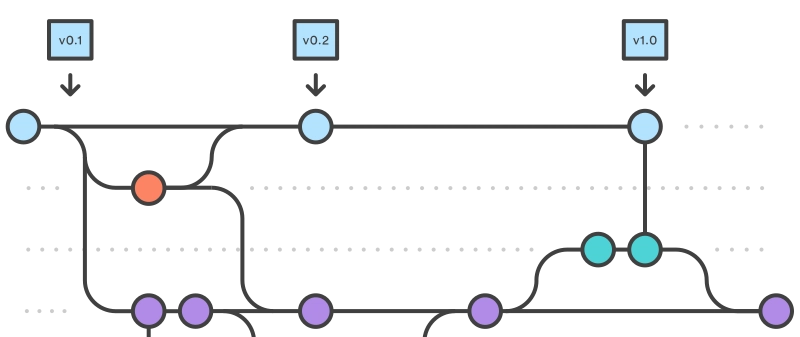
\includegraphics[width=1\textwidth]{git_branching.png}
    \caption{Git Branching and Merging Strategy Model.}
    \label{fig:git_branching}
\end{figure}

\section{Architectural Model}
Early on in the development process, the application architecture is established. It lays out the road map and best practices to adhere to in creating an organized application.

We designed a Zero-Knowledge architecture that prevents server-side access to plaintext data.

\subsection{Logical Architecture}
The choice of our system's architecture is a very important step. It is often dictated by the technical needs of our application in terms of organization and development, as well as maintenance requirements. In this context, the MVC (Model-View-Controller) architecture proves highly effective, hence our choice of the MVC architecture model presented below.

This architecture consists of separating the application components into three distinct parts: the model, the view, and the controller:
\begin{itemize}
    \item \textbf{Model}: This part of the architecture contains the application data, structured as entities using the concept of object-relational mapping. This layer interacts directly with the database.
    \item \textbf{Controller}: Located between the model and the view, this layer receives user requests, determines the processing method to trigger (including WebSocket signaling routing), and transmits the results to the corresponding view.
    \item \textbf{View}: Contains the interfaces visible in our web browser via the Next.js client, corresponding to the human-machine interface (HMI) part.
\end{itemize}

\begin{figure}[H]
    \centering
    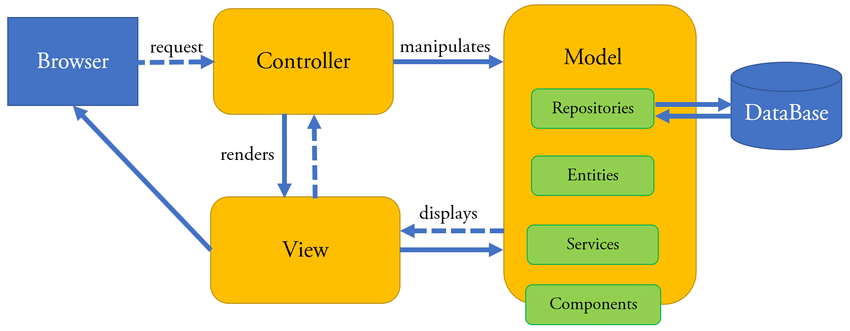
\includegraphics[width=0.85\textwidth]{mvc_architecture.png}
    \caption{MVC Architecture Model.}
    \label{fig:mvc_architecture}
\end{figure}

\subsection{Physical Architecture}
Physical architecture refers to the structure and layout of the physical components of an application.

The deployment diagram illustrates the architecture of a distributed application involving multiple components and services. The backend application contains the signaling controllers and routing logic, which communicate with the database for persistent storage. In parallel, an end user uses a PC on which a Next.js application runs via a web browser. The client utilizes WebSockets to communicate with the server and WebRTC to establish direct Peer-to-Peer (P2P) media connections with other clients. The different interactions between these components and services ensure the overall proper functioning of the application. The figure below presents the physical P2P coupling and signaling deployment flow of our application:

\begin{figure}[H]
    \centering
    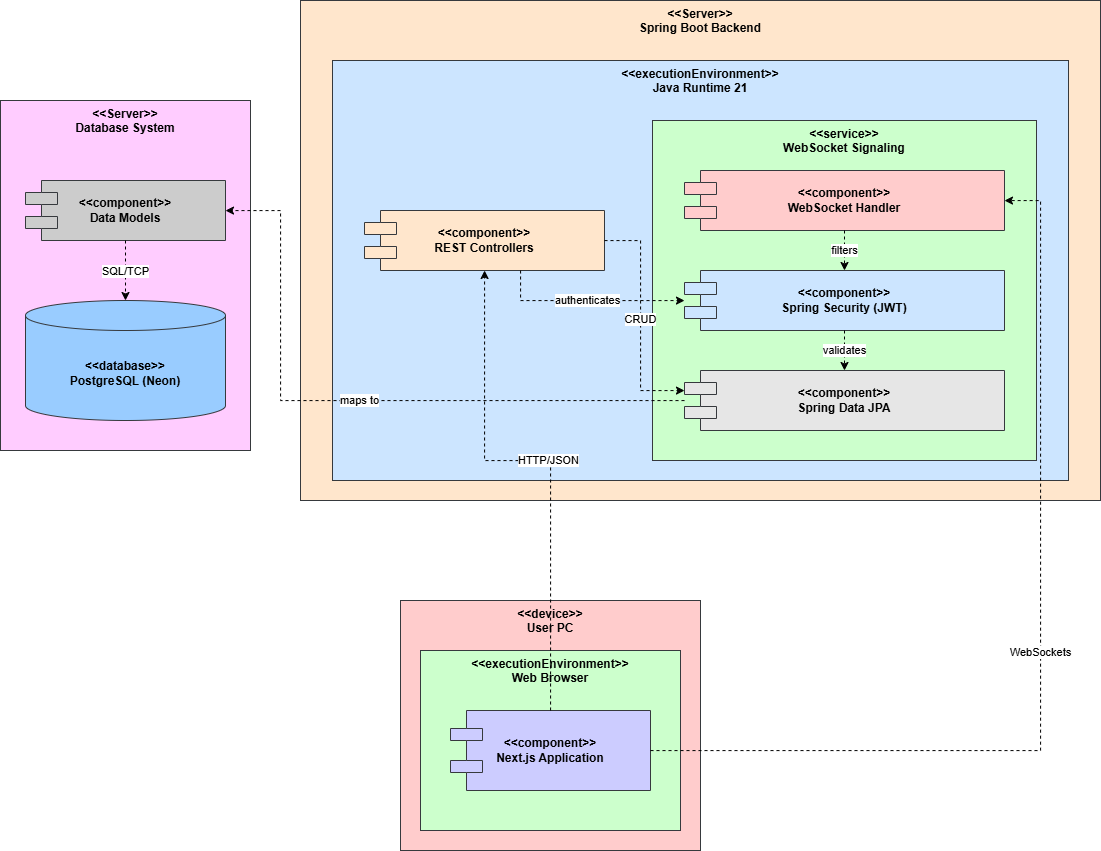
\includegraphics[width=\textwidth]{physical_architecture.png}
    \caption{Physical Component and Deployment Architecture.}
    \label{fig:physical_architecture}
\end{figure}

\section{Conclusion}
This chapter specified the user requirements, mapped security stories, detailed technology choices, and defined our core Zero-Knowledge architecture models. Chapter 3 details Release 1, focusing on authentication, key generation, and secure role isolation.
\newpage

% Chapter 3: Design
% Chapter 3: Release 1 (Cryptographic Foundations and Access Control)

\chapter{Release 1}
\label{ch:chapter3}

\section{Introduction}
This chapter details the conceptualization, design, and implementation of Release 1, which establishes the core infrastructural foundation of the platform. This release is divided into two structural sprints: Sprint 1 focuses on secure user authentication and profile management, while Sprint 2 is dedicated to server provisioning, channel architecture, and role-based access control. For each sprint, we outline the product backlog, analyze the dynamic and static system designs using UML modeling, and conclude by demonstrating the implemented interfaces that validate the functional requirements.

\section{Sprint 1}
This section presents the conceptual study and implementation of Sprint 1 of Release 1. We will focus primarily on the "Authentication" and profile management features, which ensure secure access to the platform.

\subsection{Sprint 1 Overview}
The primary objective of Sprint 1 is to implement secure credentials handling and authenticated session management. The user stories allocated to this sprint are described in Table~\ref{tab:sprint1_backlog}.

    
\renewcommand{\arraystretch}{1.5}
\begin{longtable}{| p{1.4cm} | p{10cm} | p{1.8cm} | p{1.5cm} |}
    \hline
    \rowcolor{lightgray}
    \textbf{ID} & \textbf{User Story \& Acceptance Criteria} & \textbf{Priority} & \textbf{Points} \\
    \hline
    \endfirsthead
    \hline
    \rowcolor{lightgray}
    \textbf{ID} & \textbf{User Story \& Acceptance Criteria} & \textbf{Priority} & \textbf{Points} \\
    \hline
    \endhead
    \hline
    \endfoot
    \hline
    \endlastfoot
\renewcommand{\arraystretch}{1.0} % Reset spacing for the rest of the document

    S1-01 & \textbf{As a} new user, \textbf{I want to} register an account with my email and a password, \textbf{so that} I can access the platform.
    \newline \textit{Acceptance Criteria}:
    \newline \textbullet\ Registration succeeds with valid data.
    \newline \textbullet\ Duplicate email is rejected.
    \newline \textbullet\ Password is stored securely (not in plain text). & P0 & 3 \\
    \hline
    S1-02 & \textbf{As a} registered user, \textbf{I want to} log in with my email and password, \textbf{so that} I can access my account and servers.
    \newline \textit{Acceptance Criteria}:
    \newline \textbullet\ Valid credentials return an access token.
    \newline \textbullet\ Wrong credentials are rejected with an error message.
    \newline \textbullet\ I stay logged in until I choose to log out. & P0 & 3 \\
    \hline
    S1-03 & \textbf{As a} logged-in user, \textbf{I want to} log out of my account, \textbf{so that} my session ends and no one else can use my account.
    \newline \textit{Acceptance Criteria}:
    \newline \textbullet\ Logging out clears my session.
    \newline \textbullet\ I am redirected to the text interface.
    \textbullet\ Protected pages are no longer accessible. & P1 & 1 \\
    \hline
    S1-04 & \textbf{As a} logged-in user, \textbf{I want to} view and edit my display name, \textbf{so that} other users see the name I choose.
    \newline \textit{Acceptance Criteria}:
    \newline \textbullet\ I can see my current display name.
    \newline \textbullet\ I can update it and the change is saved.
    \textbullet\ Other users see the updated name. & P1 & 2 \\
    \hline
    \caption{\textbf{Sprint 1 Backlog - Authentication \& Profile.}}
    \label{tab:sprint1_backlog} \\
\end{longtable}

\subsection{Analysis and design of sprint 1}
In this stage of Sprint 1, we will focus on the authentication implementation by carrying out a thorough analysis and outlining its conceptual design.

\subsubsection{Use case diagram}
A use case diagram illustrates the interactions between users (actors) and the system, showing the different ways in which users can engage with the system.

\begin{figure}[H]
    \centering
    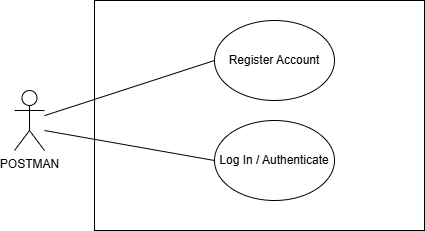
\includegraphics[width=0.8\textwidth]{use_case_sprint1_plantuml.png}
    \caption{Use Case Diagram for Sprint 1 - Authentication \& Profile.}
    \label{fig:use_case_sprint1}
\end{figure}

\subsubsection{Activity Diagram}
An activity diagram illustrates the dynamic flow of control from one activity to another, detailing the step-by-step processes of a specific use case. The figure below presents the activity diagram for the authentication process, covering both successful login and potential failure paths (e.g., invalid credentials).

\begin{figure}[H]
    \centering
    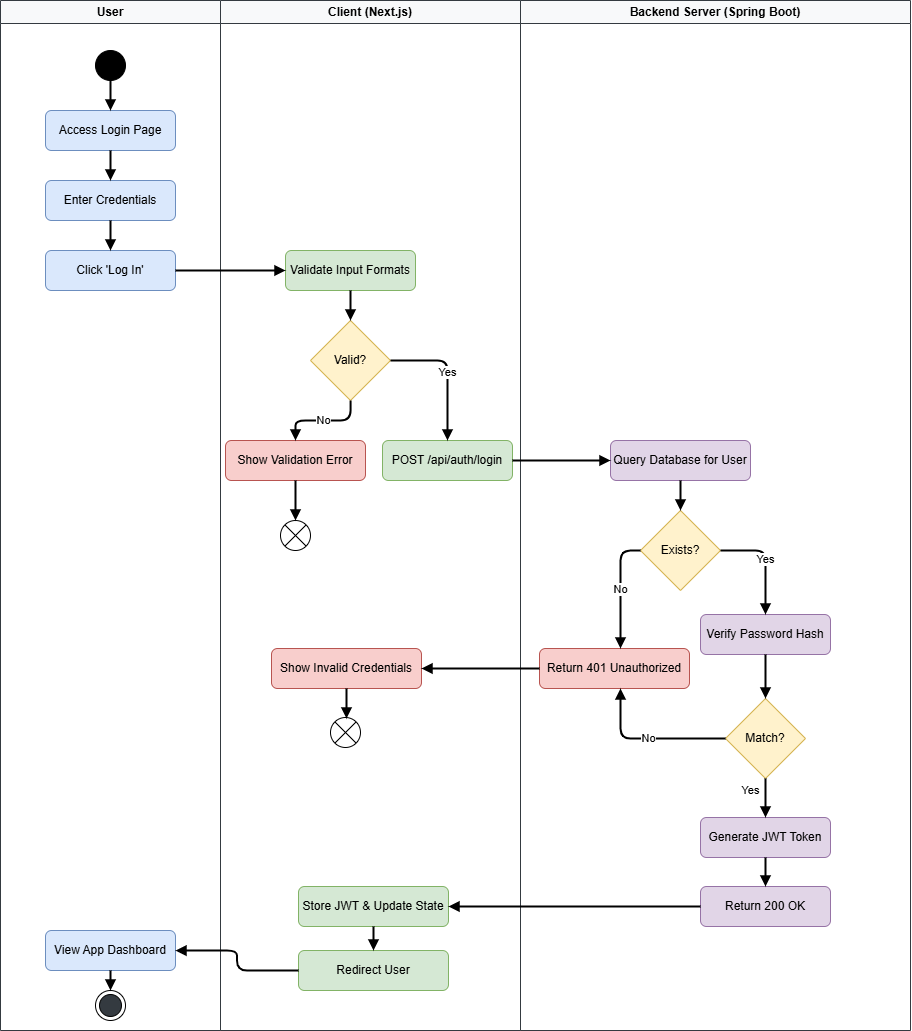
\includegraphics[width=0.9\textwidth]{auth_activity_diag.png}
    \caption{Activity Diagram for User Authentication (Success and Failure Paths).}
    \label{fig:auth_activity_sprint1}
\end{figure}

\subsubsection{Class Diagram}
The class diagram below details the static structure of the authentication entities, including the User, JWT Token, and cryptographic vault components.

\begin{figure}[H]
    \centering
    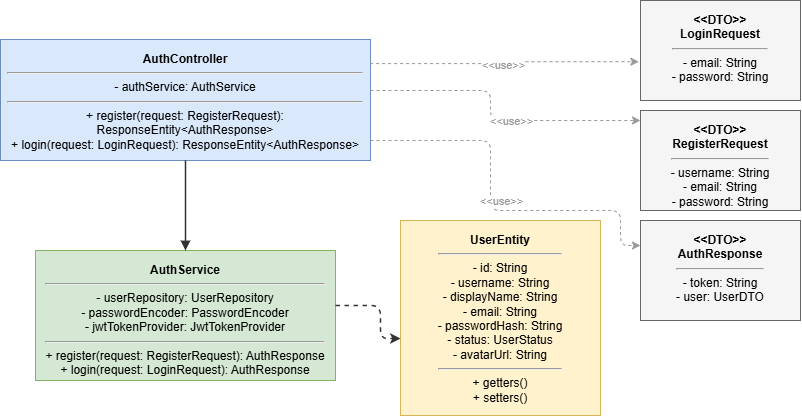
\includegraphics[width=0.8\textwidth]{auth_class_sprint1.png}
    \caption{Class Diagram for JWT Authentication.}
    \label{fig:sprint1_class_auth}
\end{figure}

\subsubsection{Design Sequence Diagram}
The sequence diagram below illustrates the operation flow and transition among the various layers of the application during the user login process:

\begin{figure}[H]
    \centering
    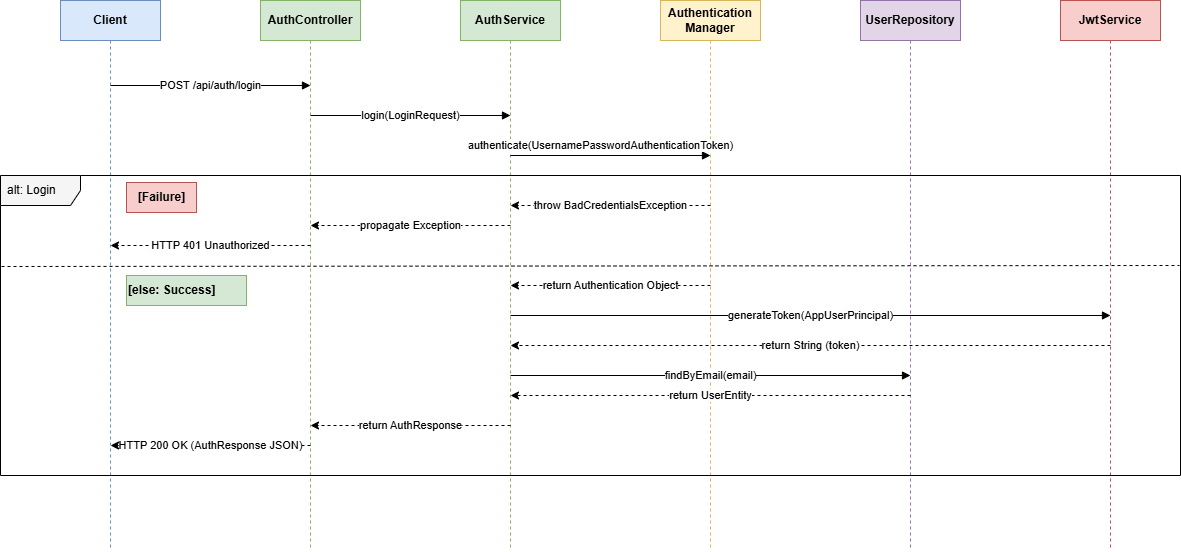
\includegraphics[width=0.9\textwidth]{seq_diag_sprint1.png}
    \caption{Secure JWT Token Exchange Sequence Diagram.}
    \label{fig:sprint1_seq_auth}
\end{figure}

\subsection{Review}
To validate the authentication process, we executed API tests using Postman. The figures below illustrate the server responses for both successful and failed login attempts.

\begin{figure}[H]
    \centering
    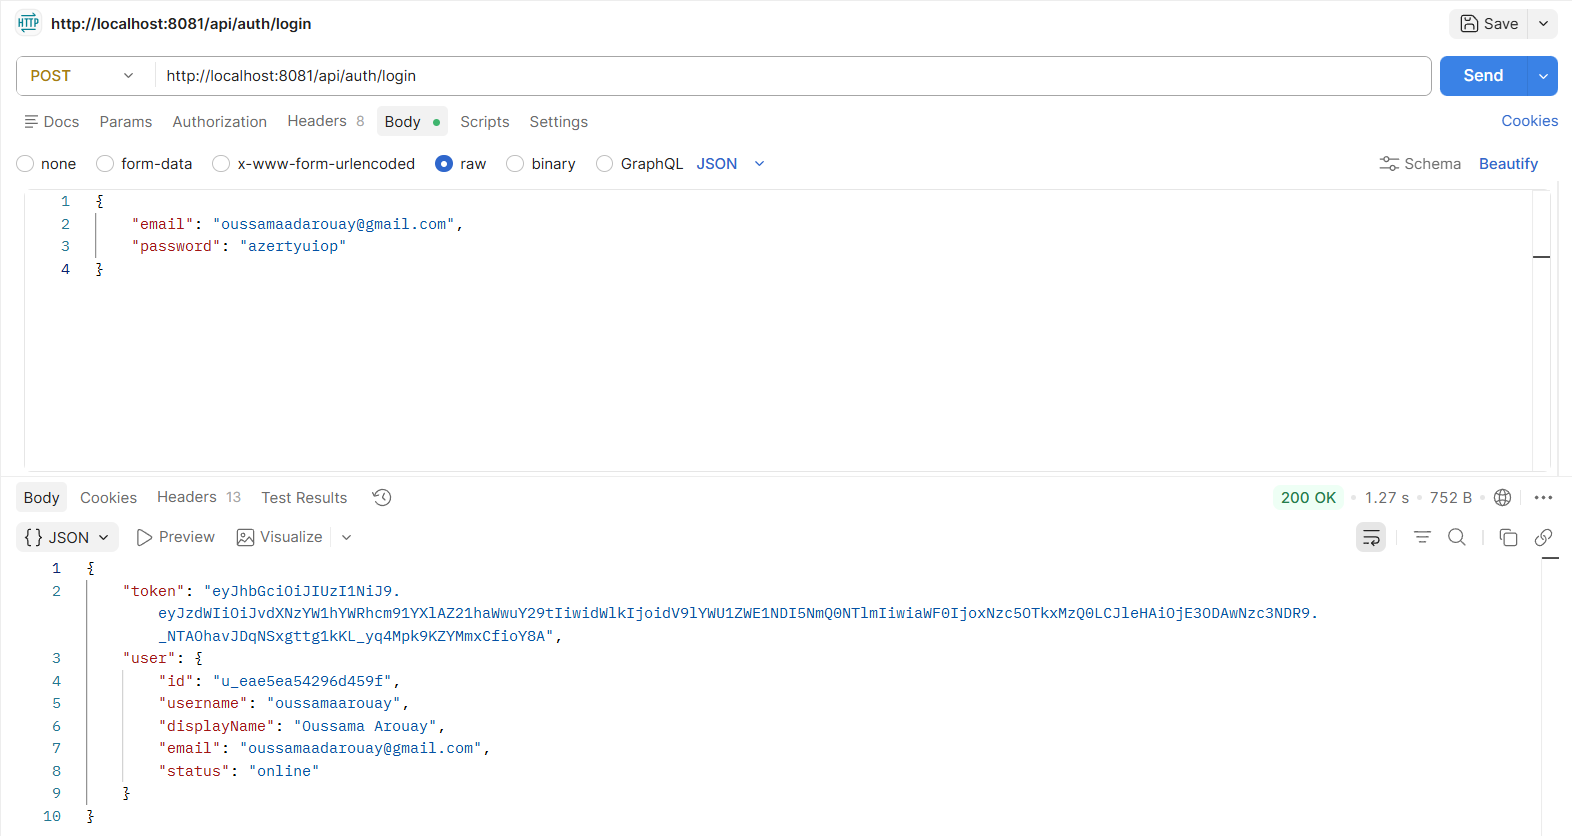
\includegraphics[width=0.8\textwidth]{login_test_success.png}
    \caption{Postman: Successful Login.}
    \label{fig:postman_login_success}
\end{figure}

\begin{figure}[H]
    \centering
    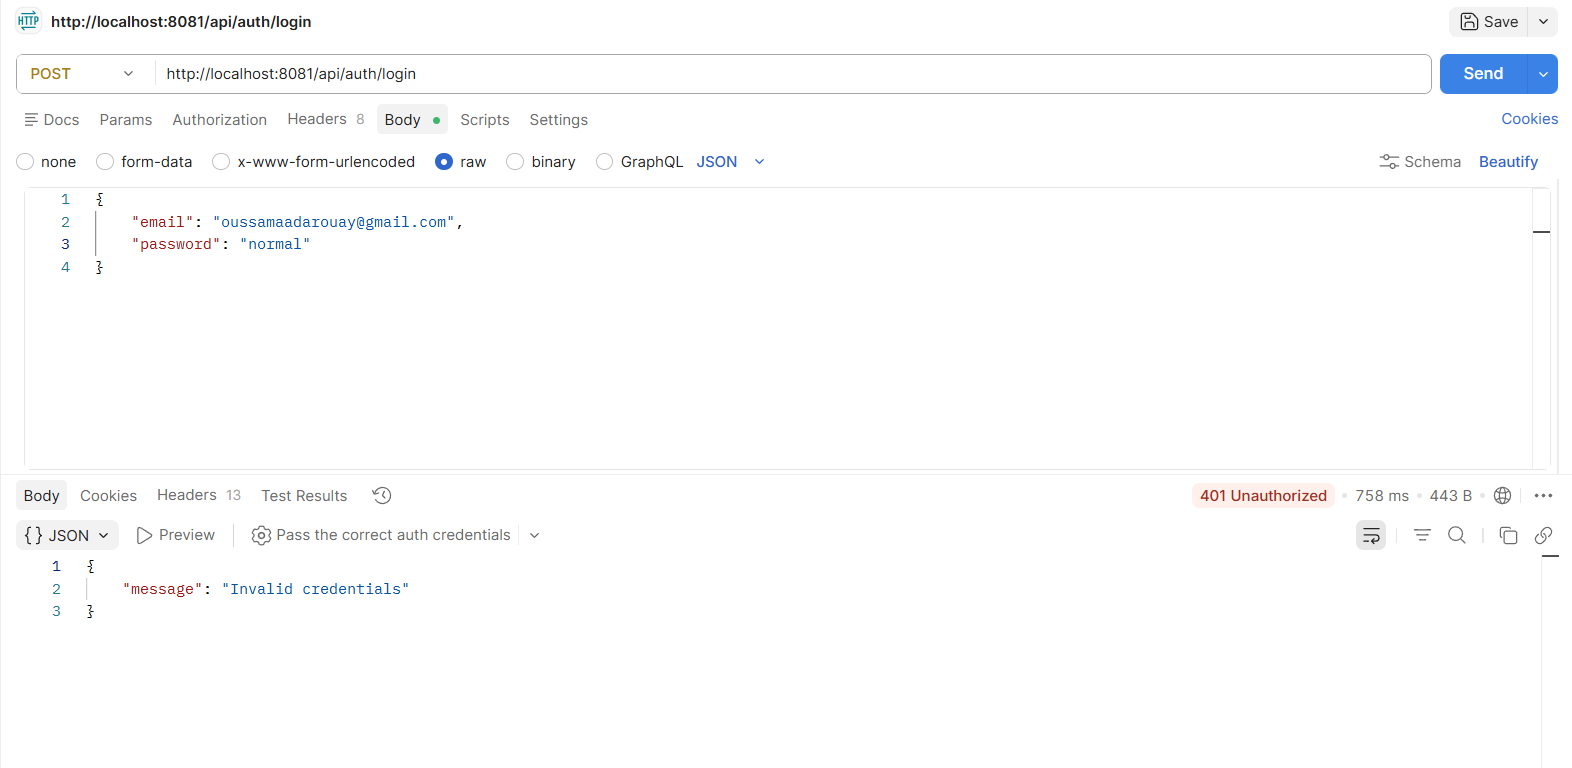
\includegraphics[width=0.8\textwidth]{login_test_failure.png}
    \caption{Postman: Failed Login Attempt (Invalid Credentials).}
    \label{fig:postman_login_failure}
\end{figure}

\section{Sprint 2: Server Management and Data Isolation}
This section presents the conceptual study and implementation of Sprint 2 of Release 1. We will focus primarily on server provisioning, channel architecture, and role-based permissions, which establish secure community workspaces within the platform.

\subsection{Sprint 2 Overview}
This sprint focuses on secure server creation, invite links, and granular channel configurations with role-based access control.

\subsection{Sprint 2 Backlog}
The primary objective of Sprint 2 is to deploy secure server configurations and member access controls. The user stories allocated to this sprint are described in Table~\ref{tab:sprint2_backlog}.

    
\renewcommand{\arraystretch}{1.5}
\begin{longtable}{| p{1.4cm} | p{10cm} | p{2.0cm} | p{1.5cm} |}
    \hline
    \rowcolor{lightgray}
    \textbf{ID} & \textbf{User Story \& Acceptance Criteria} & \textbf{Priority} & \textbf{Points} \\
    \hline
    \endfirsthead
    \hline
    \rowcolor{lightgray}
    \textbf{ID} & \textbf{User Story \& Acceptance Criteria} & \textbf{Priority} & \textbf{Points} \\
    \hline
    \endhead
    \hline
    \endfoot
    \hline
    \endlastfoot
\renewcommand{\arraystretch}{1.0} % Reset spacing for the rest of the document

    S2-01 & \textbf{As a} user, \textbf{I want to} create a new server, \textbf{so that} I have a private space to invite my friends.
    \newline \textit{Acceptance Criteria}:
    \newline \textbullet\ The server is created with the name I chose.
    \newline \textbullet\ I am automatically its owner.
    \newline \textbullet\ A default text channel is created inside it. & P0 & 3 \\
    \hline
    S2-02 & \textbf{As a} server owner, \textbf{I want to} generate an invite link for my server, \textbf{so that} I can share it with friends so they can join.
    \newline \textit{Acceptance Criteria}:
    \newline \textbullet\ A unique invite link is generated.
    \newline \textbullet\ Anyone with the link can join the server.
    \newline \textbullet\ The link expires after 24 hours. & P0 & 3 \\
    \hline
    S2-03 & \textbf{As a} user, \textbf{I want to} join a server using an invite link, \textbf{so that} I can participate in that community.
    \newline \textit{Acceptance Criteria}:
    \newline \textbullet\ Clicking a valid link adds me to the server.
    \newline \textbullet\ An expired or invalid link shows an error.
    \newline \textbullet\ I can see the server's channels after joining. & P0 & 2 \\
    \hline
    S2-04 & \textbf{As a} server owner, \textbf{I want to} create text and voice channels inside my server, \textbf{so that} I can organize conversations by topic.
    \newline \textit{Acceptance Criteria}:
    \newline \textbullet\ I can create a channel with a name and a type (text or voice).
    \newline \textbullet\ The channel appears in the server sidebar.
    \newline \textbullet\ Only the owner or admins can create channels. & P1 & 3 \\
    \hline
    S2-05 & \textbf{As a} server owner, \textbf{I want to} create roles and assign them to members, \textbf{so that} I can delegate responsibilities and control who can do what.
    \newline \textit{Acceptance Criteria}:
    \newline \textbullet\ I can create a role with a name and a set of permissions.
    \newline \textbullet\ I can assign a role to a member.
    \textbullet\ A member's permissions update immediately after assignment. & P1 & 5 \\
    \hline
    S2-06 & \textbf{As a} server member, \textbf{I want to} leave a server I no longer want to be part of, \textbf{so that} I am not in servers that are no longer relevant to me.
    \newline \textit{Acceptance Criteria}:
    \newline \textbullet\ Leaving removes me from the member list.
    \newline\textbullet\ I can no longer see the server's channels.
    \textbullet\ The server owner cannot leave without transferring ownership. & P2 & 2 \\
    \hline
    \caption{\textbf{Sprint 2 Backlog - Servers, Channels \& Permissions.}}
    \label{tab:sprint2_backlog} \\
\end{longtable}
\normalsize

\subsection{Analysis and design of sprint 2}
In this stage of Sprint 2, we focus on the architecture of server management and access control by outlining its conceptual design.

\subsubsection{Use case diagram}
The use case diagram below illustrates the interactions between authenticated users, server members, and server owners regarding the features implemented in this sprint.

\begin{figure}[H]
    \centering
    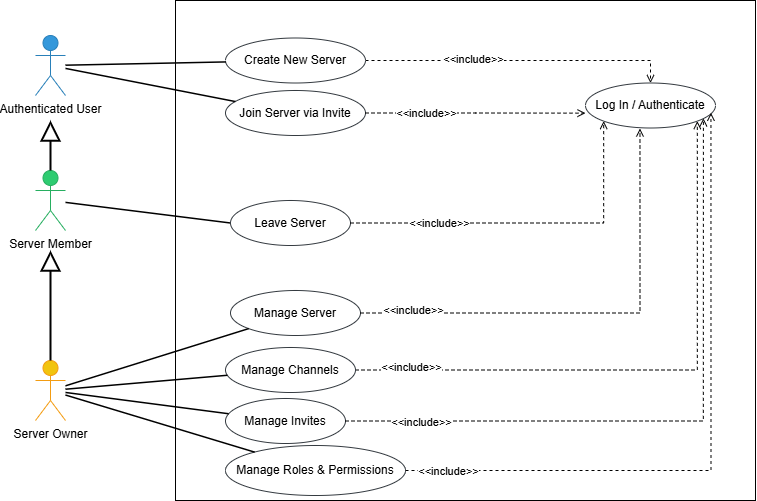
\includegraphics[width=0.8\textwidth]{UseCase_sprint2.png}
    \caption{Use Case Diagram for Sprint 2 - Server Management.}
    \label{fig:use_case_sprint2}
\end{figure}

\subsubsection{Textual Description}
At this stage, we will detail the textual descriptions of the use cases for Sprint 2 (Create a new Server/Guild and Join a Server via Invite Link) (Tables~\ref{tab:usecase_create_server} and~\ref{tab:usecase_join_server}).

\renewcommand{\arraystretch}{1.15}
\begin{table}[H]
    \centering
    \begin{tabular}{| p{3.5cm} | p{10.5cm} |}
        \hline
        \textbf{Use Case} & Create a new Server/Guild \\
        \hline
        \textbf{Actor} & Authenticated User \\
        \hline
        \textbf{Pre-condition} & The actor must be logged into the platform with a valid session. \\
        \hline
        \textbf{Main Scenario} & 
        \vspace{-0.3cm}
        \begin{minipage}[t]{10.5cm}
            \begin{enumerate}
                \item The actor clicks on the "+" sign in the sidebar.
                \item The system prompts the actor to enter a server name.
                \item The actor submits the creation form.
                \item The system registers the new server in the database and assigns the actor as the "Owner".
                \item The system automatically generates a default "general" text channel.
            \end{enumerate}
            \vspace{0.1cm}
        \end{minipage} \\
        \hline
        \textbf{Post-condition} & A new server is created, and the user is granted absolute Owner privileges over it. \\
        \hline
    \end{tabular}
    \vspace{0.2cm}
    \caption{Textual description of "Create a new Server/Guild"}
    \label{tab:usecase_create_server}
\end{table}


\renewcommand{\arraystretch}{1.15}
\begin{table}[H]
    \centering
    \begin{tabular}{| p{3.5cm} | p{10.5cm} |}
        \hline
        \textbf{Use Case} & Join a Server via Invite Link \\
        \hline
        \textbf{Actor} & Authenticated User \\
        \hline
        \textbf{Pre-condition} & The actor is logged in, possesses a valid invite link, and is not already a member of the server. \\
        \hline
        \textbf{Main Scenario} & 
        \vspace{-0.5cm}
        \begin{minipage}[t]{10.5cm}
            \begin{enumerate}
                \item The actor clicks on a server invite link.
                \item The system validates the invite link (checks if it exists and has not expired).
                \item The system verifies that the actor is not already a member of the server.
                \item The system adds the actor to the server's member list.
                \item The system assigns the actor default roles for that server.
            \end{enumerate}
            \vspace{-0.2cm}
        \end{minipage} \\
        \hline
        \textbf{Post-condition} & The actor becomes a member of the server and gains access to its default channels. \\
        \hline
    \end{tabular}
    \vspace{0.2cm}
    \caption{Textual description of "Join Server via Invite"}
    \label{tab:usecase_join_server}
\end{table}
\renewcommand{\arraystretch}{1.0}


\subsubsection{Class Diagram}
The class diagram below illustrates the relationships between Servers, Channels, Roles, and Permissions, highlighting how cryptographic keys are associated with server entities.

\begin{figure}[H]
    \centering
    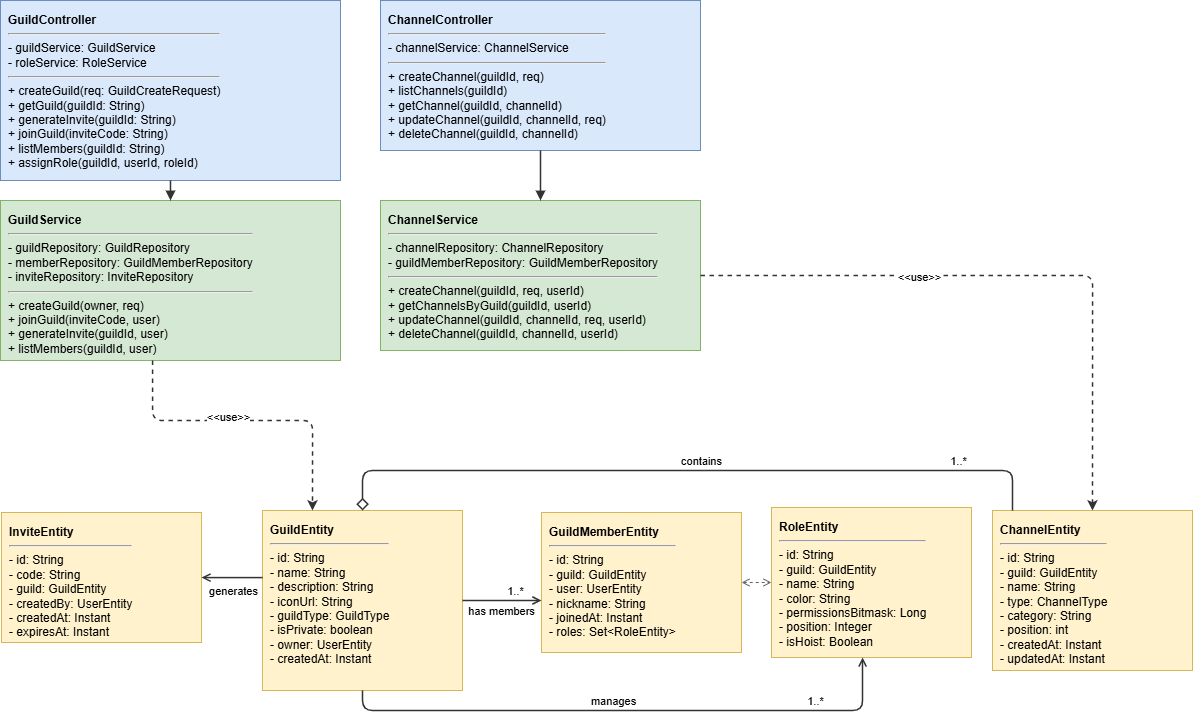
\includegraphics[width=0.8\textheight, angle=90]{class_diag_sprint2.png}
    \caption{Class Diagram for Sprint 2.}
    \label{fig:sprint2_class_perms}
\end{figure}
\subsection{Sprint 2 Review}
To validate the backend logic and operations developed during Sprint 2, we executed API tests using Postman. The figures below illustrate the successful execution of server creation, joining a server via an invite link, and creating a text channel.

\begin{figure}[H]
    \centering
    \includegraphics[width=0.8\textwidth]{{guild_creation.png}}
    \caption{Postman: Server Creation Process.}
    \label{fig:sprint2_guild_create}
\end{figure}

\begin{figure}[H]
    \centering
    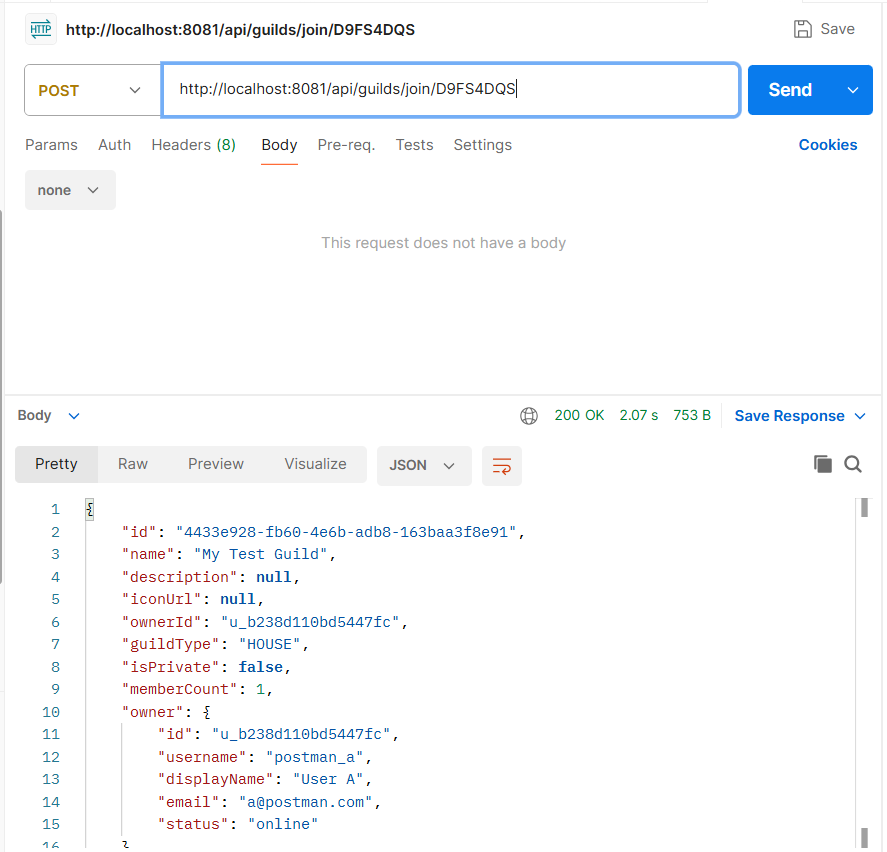
\includegraphics[width=0.8\textwidth]{guildjoin.png}
    \caption{Postman: Joining a Server via Invite.}
    \label{fig:sprint2_guild_join}
\end{figure}

\begin{figure}[H]
    \centering
    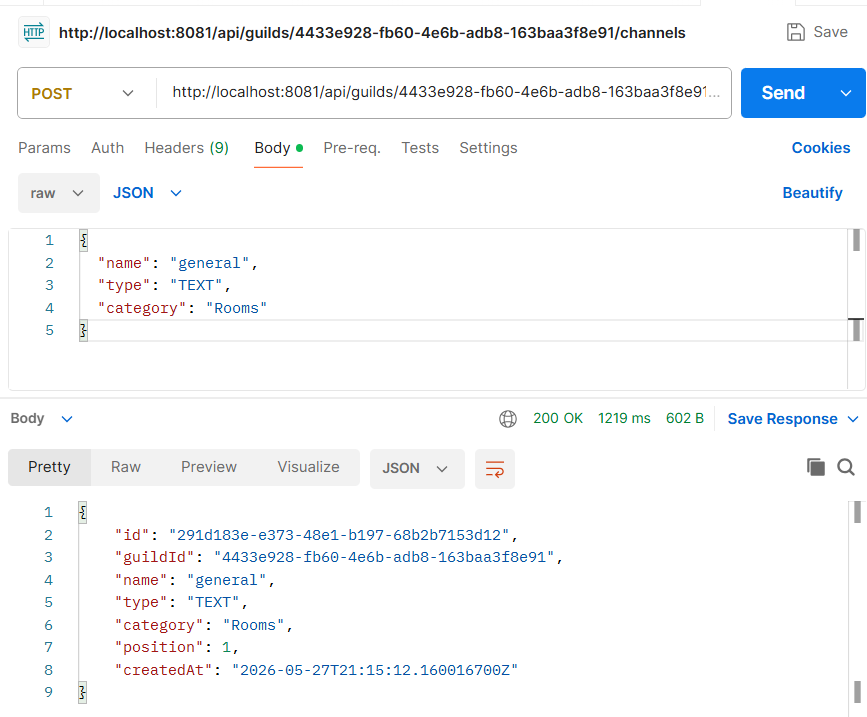
\includegraphics[width=0.8\textwidth]{textchannel creation.png}
    \caption{Postman: Creating a Text Channel.}
    \label{fig:sprint2_channel_create}
\end{figure}


\section{Conceptual Design of Release 1}

\subsection{Data Modeling}
In this section, we present the entities and tables that make up the structural foundation of our platform for this release. The data model covers user authentication, server provisioning, and role-based access control. Table~\ref{tab:data_dictionary_r1} presents the data dictionary.

\renewcommand{\arraystretch}{1.5}
\begin{longtable}{| p{4cm} | p{3.5cm} | p{7cm} |}
    \hline
    \rowcolor{lightgray}
    \textbf{Entity} & \textbf{Attribute} & \textbf{Description} \\
    \hline
    \endfirsthead
    \hline
    \rowcolor{lightgray}
    \textbf{Entity} & \textbf{Attribute} & \textbf{Description} \\
    \hline
    \endhead
    \hline
    \endfoot
    \hline
    \caption{Dictionnaire de données de la release 1.}
    \label{tab:data_dictionary_r1}
    \endlastfoot

    User (Utilisateur) & id & Unique identifier for the user. \\
    \cline{2-3}
         & email & User's email address. \\
    \cline{2-3}
         & username & User's chosen display name. \\
    \cline{2-3}
         & passwordHash & Hashed password for authentication. \\
    \cline{2-3}
         & status & Current presence status (e.g., Online, Offline). \\
    \cline{2-3}
         & dateCreated & Account creation date. \\
    \hline
    Server (Serveur) & id & Unique identifier for the server. \\
    \cline{2-3}
         & name & Name of the server. \\
    \cline{2-3}
         & ownerId & Identifier of the user who owns the server. \\
    \cline{2-3}
         & iconUrl & URL to the server's icon image. \\
    \cline{2-3}
         & dateCreated & Creation date of the server. \\
    \hline
    Channel (Canal) & id & Unique identifier for the channel. \\
    \cline{2-3}
         & serverId & Identifier of the parent server. \\
    \cline{2-3}
         & name & Name of the channel (e.g., "general"). \\
    \cline{2-3}
         & type & Type of the channel (text or voice). \\
    \cline{2-3}
         & dateCreated & Creation date of the channel. \\
    \hline
    Role (Rôle) & id & Unique identifier for the role. \\
    \cline{2-3}
         & serverId & Identifier of the server the role belongs to. \\
    \cline{2-3}
         & name & Name of the role (e.g., "Admin", "Member"). \\
    \cline{2-3}
         & permissions & Access control permissions string or bitfield. \\
    \hline
    ServerMember (Membre) & userId & Identifier of the user. \\
    \cline{2-3}
         & serverId & Identifier of the server. \\
    \cline{2-3}
         & roleId & Identifier of the assigned role. \\
    \cline{2-3}
         & joinedAt & Date the user joined the server. \\
    \hline
\end{longtable}
\renewcommand{\arraystretch}{1.0}

\begin{figure}[H]
    \centering
    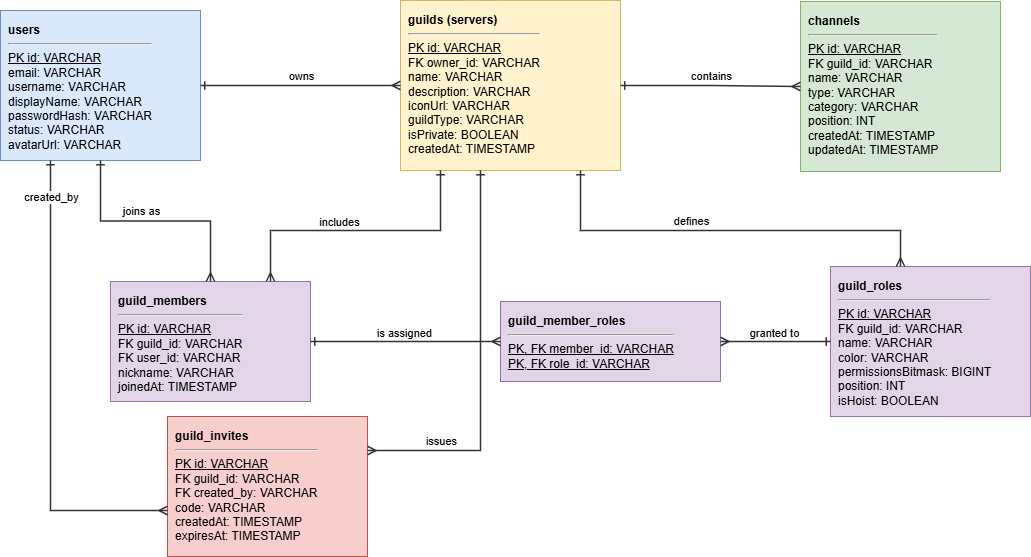
\includegraphics[width=1.1\textwidth]{release1_modele_logique_donne.png}
    \caption{Logical Data Model (MLD) for Release 1.}
    \label{fig:r1_mld}
\end{figure}

\subsubsection{Design Sequence Diagram}
We illustrate here the operation flow and transition among the various layers of an application through design sequence diagrams in this section.



\subsection{Graphical Design}
Graphical design, otherwise referred to as visual design, is an important part of visual product creation including websites, mobile apps, user interfaces, posters, logos, and ads.
In this section, we show mockup examples of our application to meet user requirements and improve user experience on a particular page.

The following figures showcase the visual design of the platform's key interfaces developed during Release 1.

\begin{figure}[H]
    \centering
    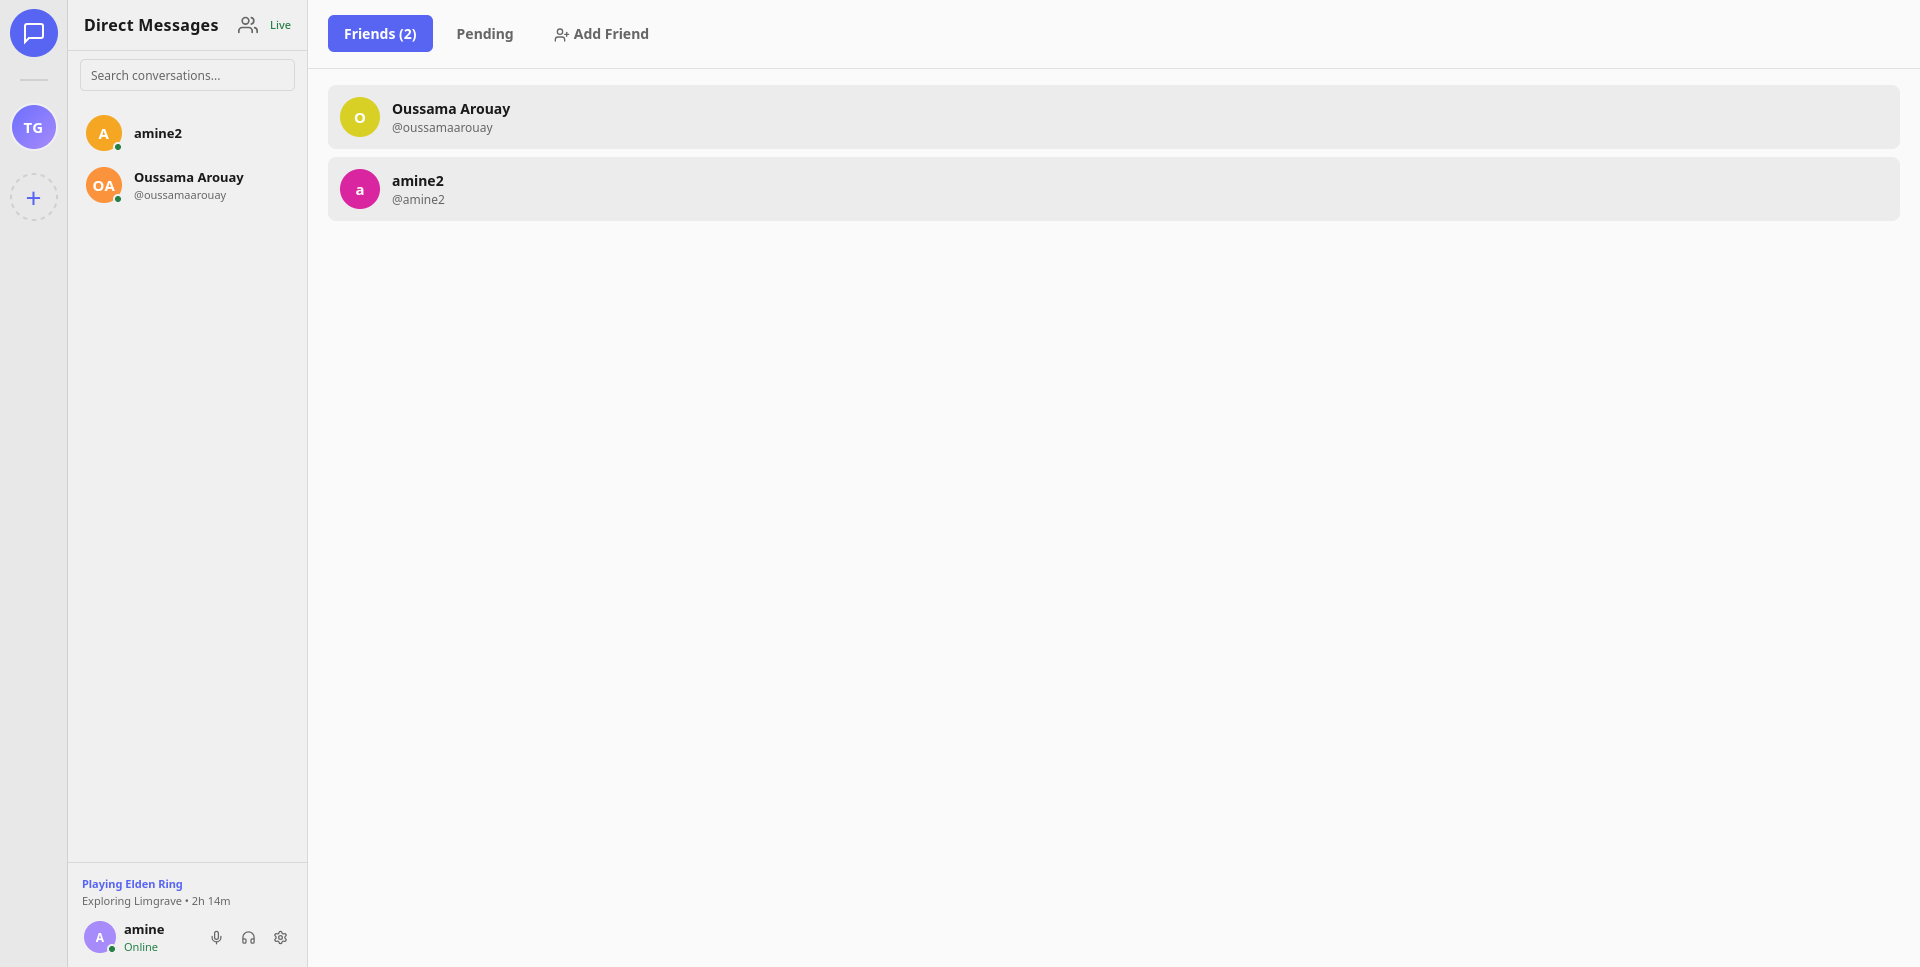
\includegraphics[width=0.85\textwidth]{landing_page_light.png}
    \caption{Mockup: Landing Page Design.}
    \label{fig:ui_landing_page}
\end{figure}

\begin{figure}[H]
    \centering
    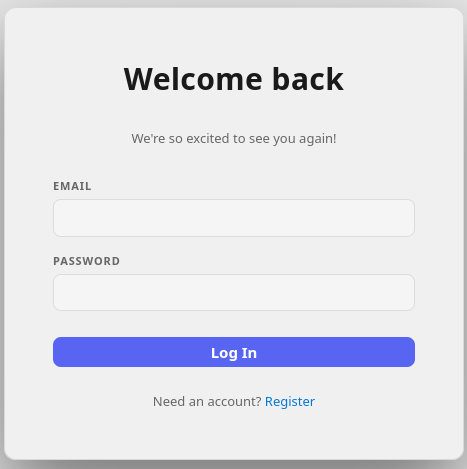
\includegraphics[width=0.5\textwidth]{login.png}
    \caption{Mockup: Login Interface.}
    \label{fig:ui_login}
\end{figure}

\begin{figure}[H]
    \centering
    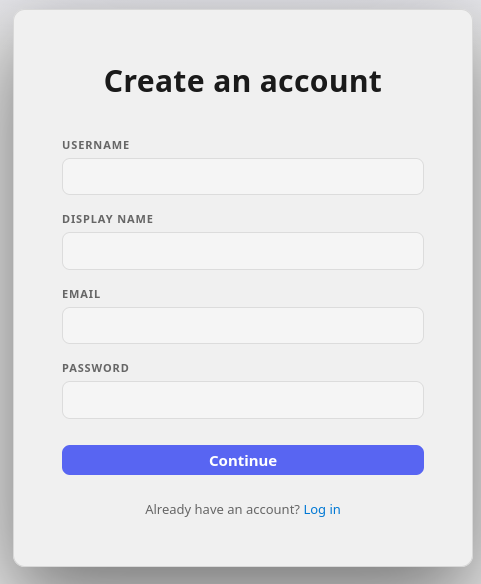
\includegraphics[width=0.5\textwidth]{singup.png}
    \caption{Mockup: Registration Interface.}
    \label{fig:ui_signup}
\end{figure}

\begin{figure}[H]
    \centering
    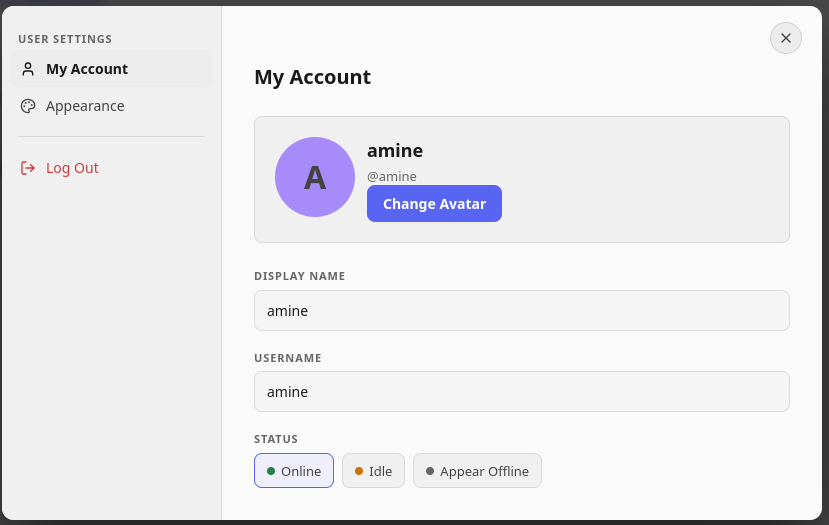
\includegraphics[width=0.5\textwidth]{user_settings.png}
    \caption{Mockup: User Settings and Profile Management.}
    \label{fig:ui_user_settings}
\end{figure}

\begin{figure}[H]
    \centering
    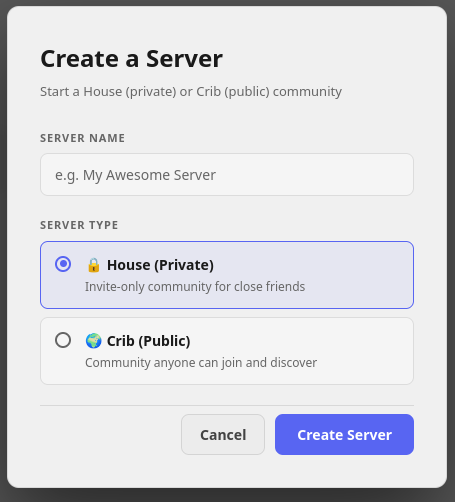
\includegraphics[width=0.4\textwidth]{create_guild.png}
    \caption{Mockup: Server Creation Interface.}
    \label{fig:ui_create_guild}
\end{figure}

\begin{figure}[H]
    \centering
    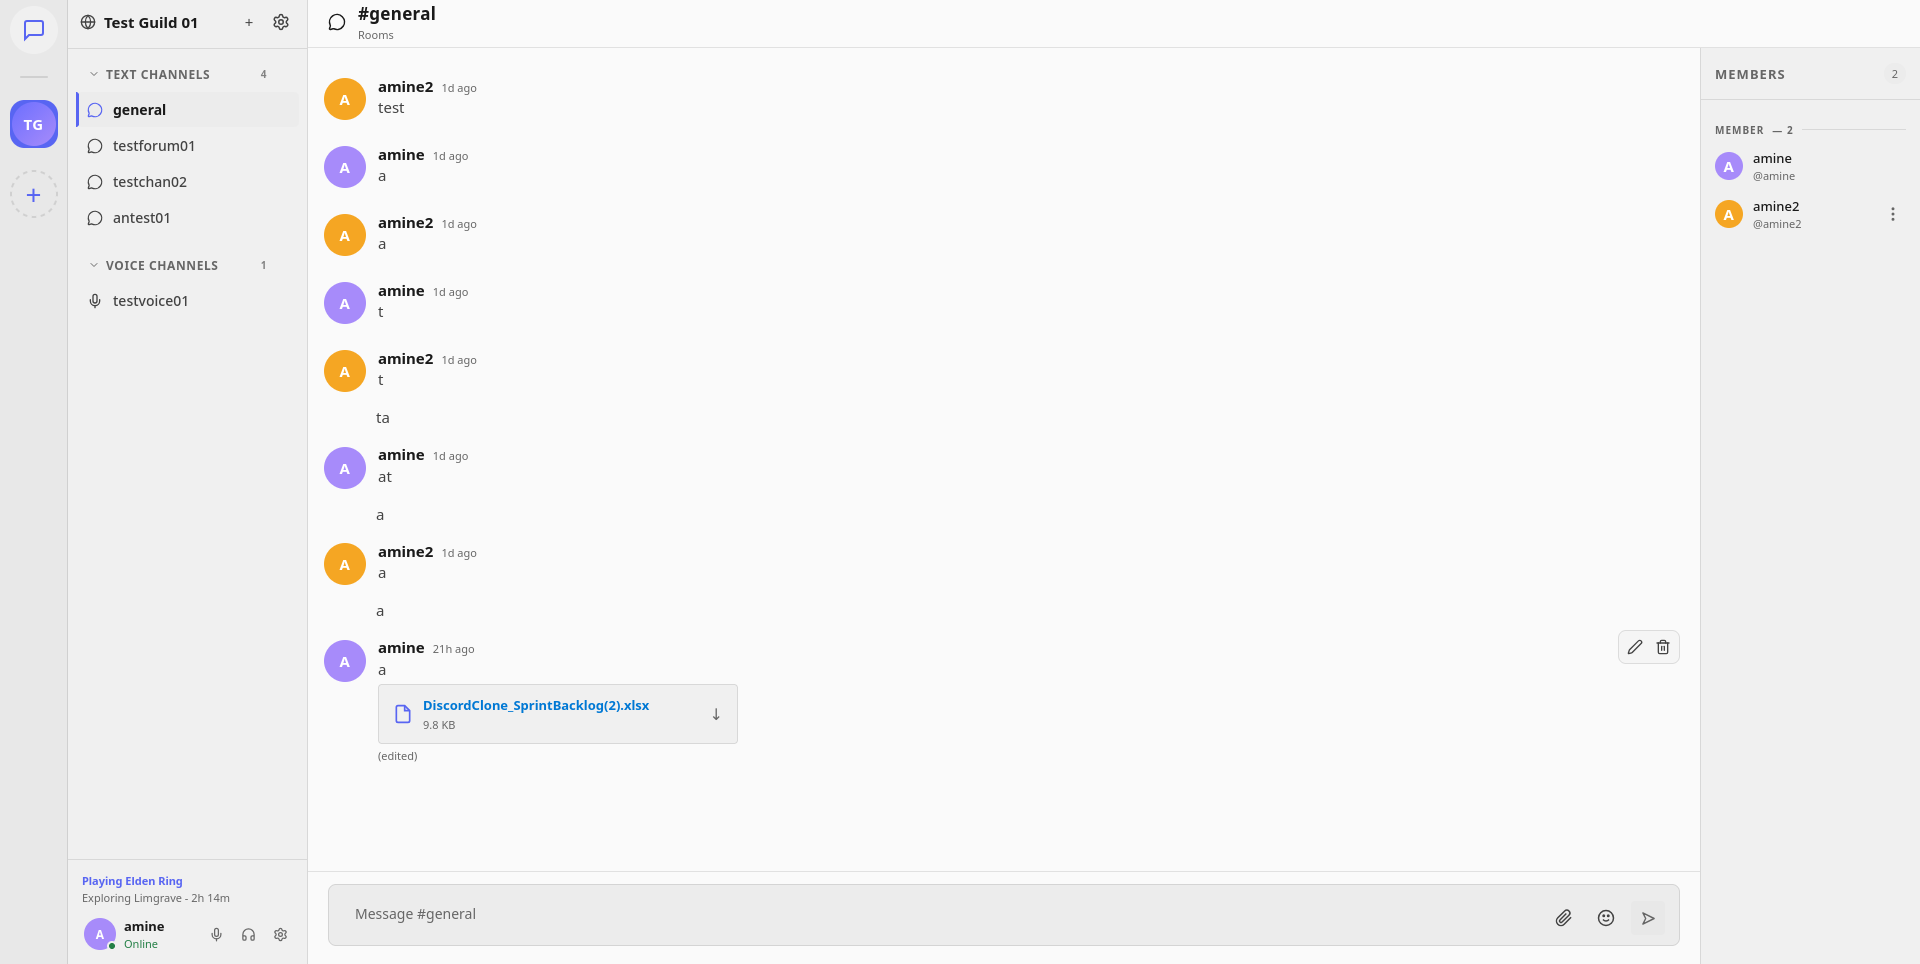
\includegraphics[width=0.85\textwidth]{main_guild_view.png}
    \caption{Mockup: Main Server View and Channel Navigation.}
    \label{fig:ui_main_guild_view}
\end{figure}

\begin{figure}[H]
    \centering
    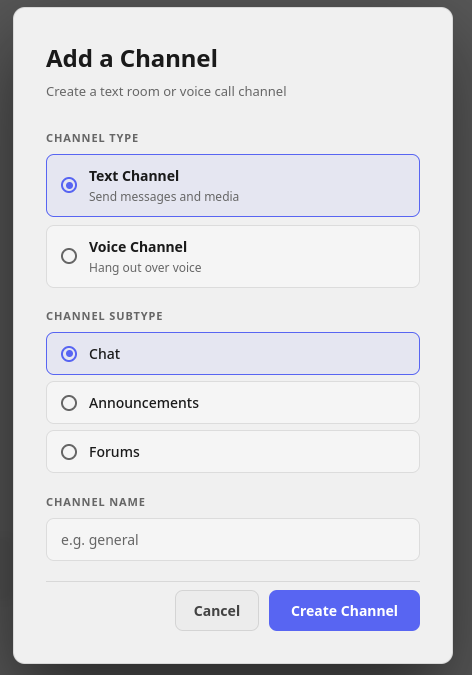
\includegraphics[width=0.5\textwidth]{add_text_channel.png}
    \caption{Mockup: Creating a Text Channel.}
    \label{fig:ui_add_text_channel}
\end{figure}

\begin{figure}[H]
    \centering
    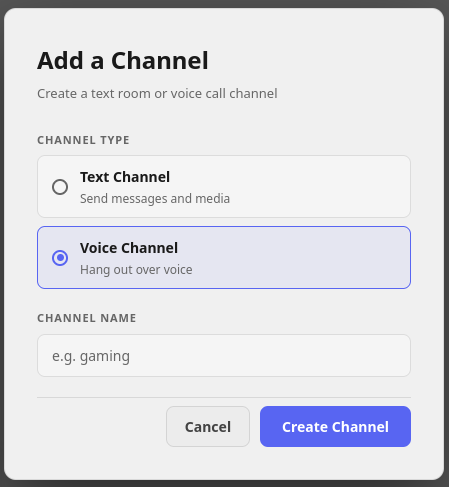
\includegraphics[width=0.5\textwidth]{add_voice_channel.png}
    \caption{Mockup: Creating a Voice Channel.}
    \label{fig:ui_add_voice_channel}
\end{figure}

\begin{figure}[H]
    \centering
    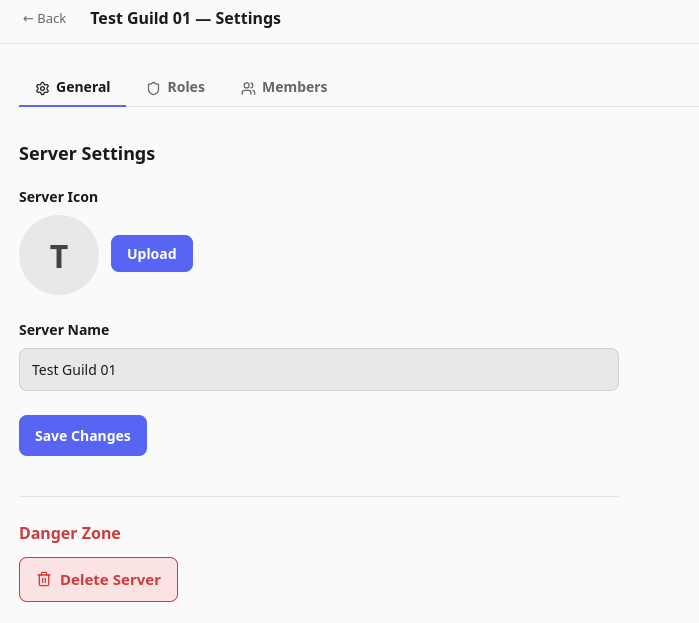
\includegraphics[width=0.5\textwidth]{guild_settings.png}
    \caption{Mockup: Server Settings Overview.}
    \label{fig:ui_guild_settings}
\end{figure}

\begin{figure}[H]
    \centering
    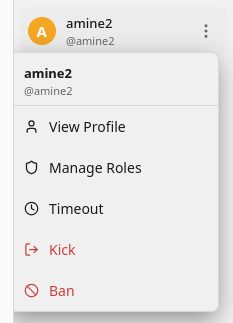
\includegraphics[width=0.3\textwidth]{guild_member_dropdown.png}
    \caption{Mockup: Member Action Menu.}
    \label{fig:ui_member_dropdown}
\end{figure}

\begin{figure}[H]
    \centering
    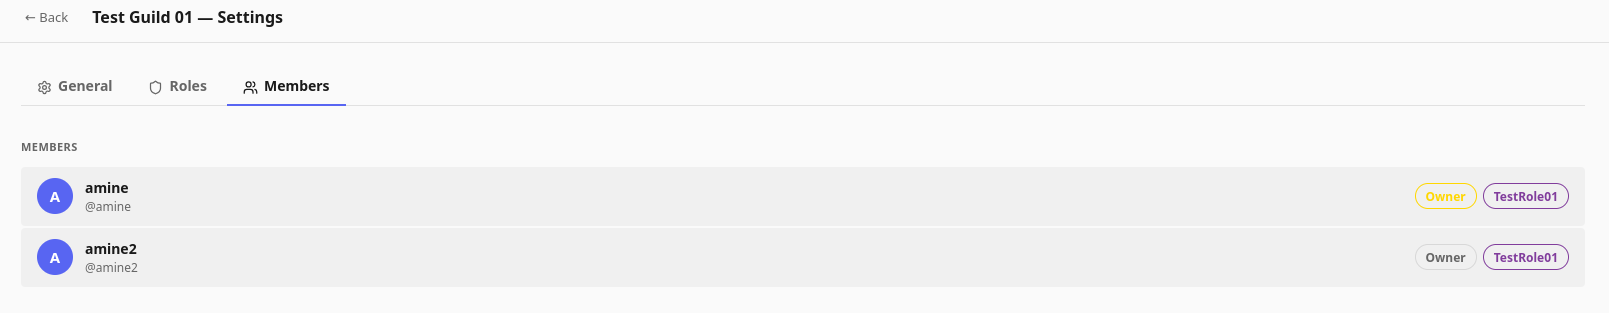
\includegraphics[width=0.5\textwidth]{guild_members_settings.png}
    \caption{Mockup: Member Management Interface.}
    \label{fig:ui_guild_members}
\end{figure}

\begin{figure}[H]
    \centering
    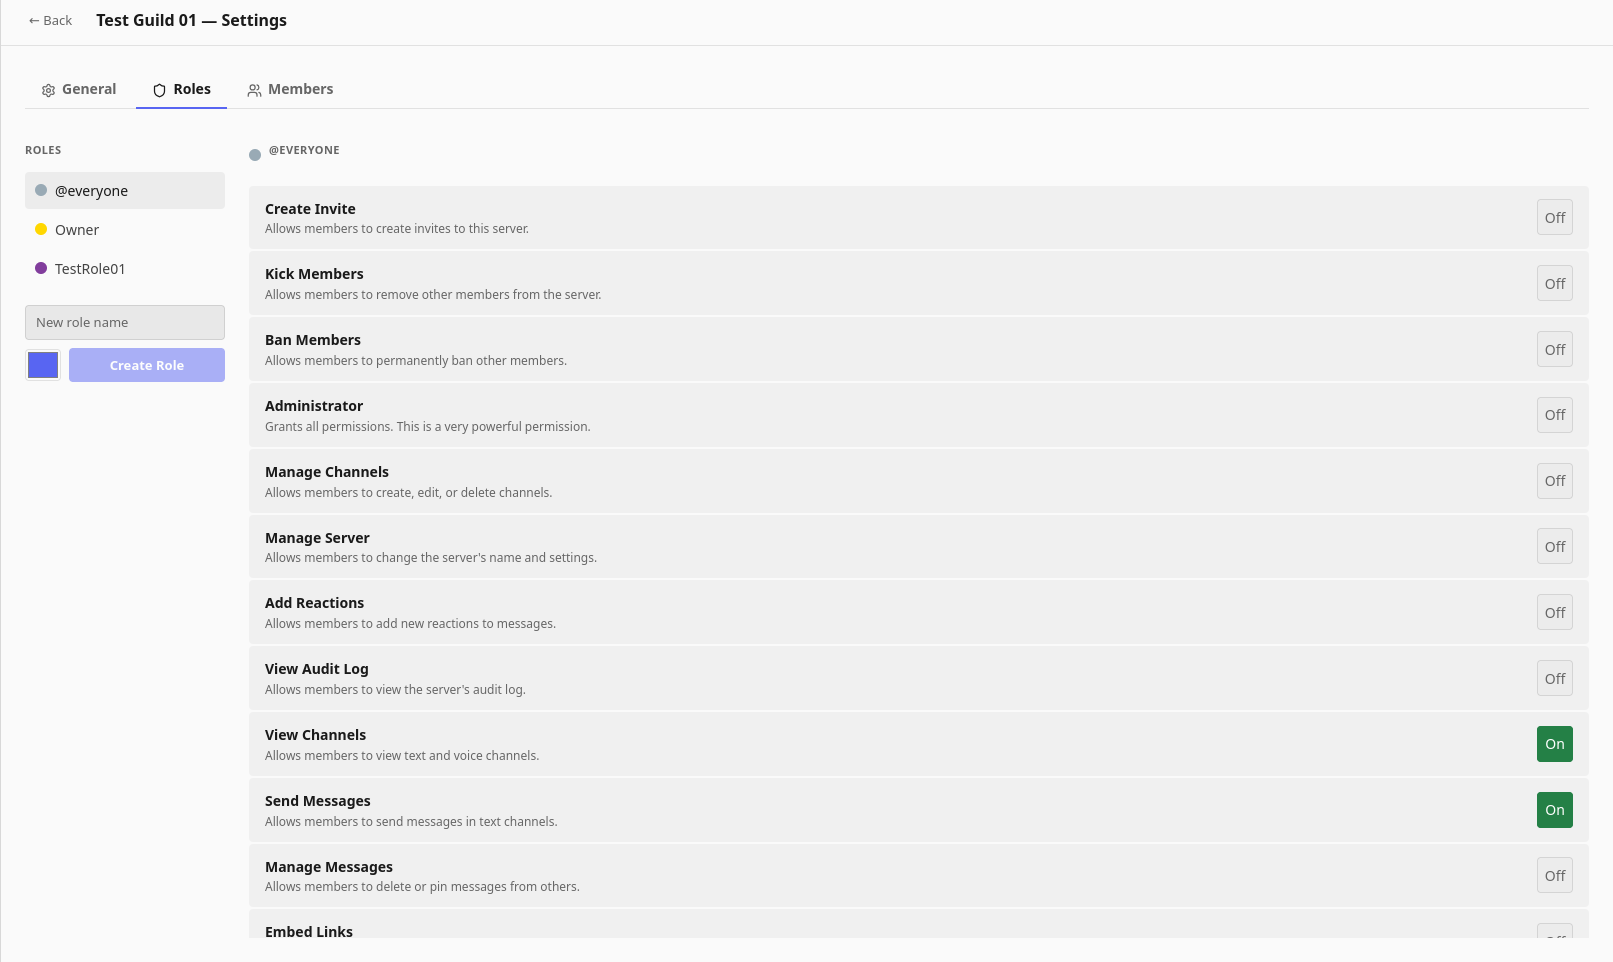
\includegraphics[width=0.5\textwidth]{guild_roles_settings.png}
    \caption{Mockup: Role Management Interface.}
    \label{fig:ui_guild_roles}
\end{figure}

\begin{figure}[H]
    \centering
    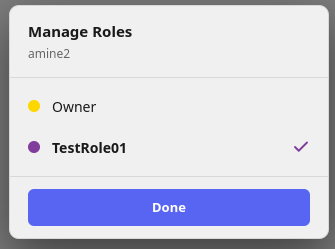
\includegraphics[width=0.4\textwidth]{member_manage_role.png}
    \caption{Mockup: Role Management and Member Administration.}
    \label{fig:ui_member_manage_role}
\end{figure}

\section{Conclusion}
This chapter presented Release 1 of our platform. By implementing secure authentication in Sprint 1 and server management with role-based access control in Sprint 2, we established the foundational infrastructure required for the encrypted messaging and P2P voice features detailed in Chapter 4.
\newpage

% Chapter 4: Implementation, Testing, and Deployment
% Chapter 4: Release 2 (End-to-End Encrypted Communication and P2P)

\chapter{Release 2}
\label{ch:chapter4}

\section{Introduction}
This chapter details the conceptualization, design, and implementation of Release 2, which constitutes the most critical phase of our project by establishing its core security and privacy features. This release is divided into three highly specialized sprints: Sprint 3 focuses on securing text communications through robust AES-256-GCM encryption, Sprint 4 is dedicated to engineering a secure Peer-to-Peer (P2P) WebRTC voice calling architecture that bypasses centralized media servers, and Sprint 5 ensures transparency and usability through open-source self-hosting capabilities and extended UI features. For each sprint, we outline the product backlog, analyze the dynamic and static system designs using UML modeling, and conclude by demonstrating the implemented functionalities that validate our rigorous security requirements.

\section{Sprint 3}

\subsection{Sprint 3 Overview}
The objective of this sprint is to establish real-time encrypted messaging and instant chat history delivery. The user stories allocated to this sprint are described in Table~\ref{tab:sprint3_backlog}.


\renewcommand{\arraystretch}{1.5}
\begin{longtable}{| p{1.4cm} | p{10cm} | p{2.0cm} | p{1.5cm} |}
    \hline
    \rowcolor{lightgray}
    \textbf{ID} & \textbf{User Story \& Acceptance Criteria} & \textbf{Priority} & \textbf{Points} \\
    \hline
    \endfirsthead
    \hline
    \rowcolor{lightgray}
    \textbf{ID} & \textbf{User Story \& Acceptance Criteria} & \textbf{Priority} & \textbf{Points} \\
    \hline
    \endhead
    \hline
    \endfoot
    \hline
    \endlastfoot
\renewcommand{\arraystretch}{1.0} % Reset spacing for the rest of the document

    S3-01 & \textbf{As a} server member, \textbf{I want to} send a message in a text channel and have everyone see it instantly, \textbf{so that} we can have a real-time conversation.
    \newline \textit{Acceptance Criteria}:
    \newline \textbullet\ Messages appear for all members of the channel without refreshing.
    \newline \textbullet\ Message includes my name and the time it was sent.
    \newline \textbullet\ An empty message cannot be sent. & P0 & 8 \\
    \hline
    S3-02 & \textbf{As a} server member, \textbf{I want to} see recent messages when I open a channel, \textbf{so that} I can catch up on what was discussed before I arrived.
    \newline \textit{Acceptance Criteria}:
    \newline \textbullet\ The last 50 messages load when I open a channel.
    \newline \textbullet\ Messages are shown in chronological order.
    \newline \textbullet\ Each message shows the sender's name and timestamp. & P1 & 3 \\
    \hline
    S3-03 & \textbf{As a} server member, \textbf{I want to} see which members of a server are online or offline, \textbf{so that} I know who is available to chat.
    \newline \textit{Acceptance Criteria}:
    \newline \textbullet\ Online members are visually distinct from offline ones.
    \newline \textbullet\ My status becomes online when I log in.
    \newline \textbullet\ My status becomes offline when I close the app. & P1 & 3 \\
    \hline
    S3-04 & \textbf{As a} server member, \textbf{I want to} edit my own messages after sending them, \textbf{so that} I can fix mistakes.
    \newline \textit{Acceptance Criteria}:
    \newline \textbullet\ I can edit the text of a message I sent.
    \newline \textbullet\ The message shows an 'edited' label.
    \newline \textbullet\ Other members cannot edit my messages. & P1 & 2 \\
    \hline
    S3-05 & \textbf{As a} server member, \textbf{I want to} delete my own messages, \textbf{so that} I can remove something I no longer want to have posted.
    \newline \textit{Acceptance Criteria}:
    \newline \textbullet\ My message disappears for all members.
 \newline \textbullet\ I can only delete my own messages unless I have a moderation role.
    \newline \textbullet\ Deletion is immediate and cannot be undone. & P1 & 2 \\
    \hline
    \caption{\textbf{Sprint 3 Backlog - Real-Time Chat \& Presence.}}
    \label{tab:sprint3_backlog}
\end{longtable}
\normalsize

\subsection{Designing the Static View}
The static view of a system focuses on its structural aspects, such as the entities it manages and the relationships among them.

\subsubsection{Use Case Diagram}
The following diagram highlights the core interactions introduced in this sprint, specifically focusing on the sending of messages and related functionalities.

\begin{figure}[H]
    \centering
    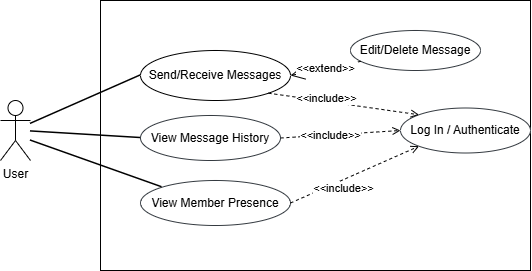
\includegraphics[width=0.9\textwidth]{UseCaseGeneral-send_message_sprint3.png}
    \caption{Use Case Diagram: Sending a Message (Sprint 3).}
    \label{fig:usecase_sprint3}
\end{figure}


\subsection{Cryptographic Algorithm Selection}

When designing the encryption pipeline to guarantee the confidentiality and integrity of messages at rest, several cryptographic algorithms were evaluated. Table~\ref{tab:crypto_comparison} outlines the comparison between the considered options:

\renewcommand{\arraystretch}{1.15}
\begin{table}[H]
    \centering
    \small
    \begin{tabular}{| p{3cm} | p{2.2cm} | p{2.8cm} | p{6.5cm} |}
        \hline
        \rowcolor{lightgray}
        \textbf{Algorithm} & \textbf{Type} & \textbf{Integrity Check} & \textbf{Drawbacks / Fit} \\
        \hline
        \textbf{AES-256-GCM} & Symmetric (AEAD) & Built-in (Auth Tag) & Hardware accelerated (AES-NI), extremely fast, and provides built-in tampering protection. \\
        \hline
        \textbf{AES-256-CBC} & Symmetric Block & None (Requires HMAC) & Requires padding; vulnerable to padding oracle attacks without strict MAC implementations. \\
        \hline
        \textbf{ChaCha20-Poly1305} & Symmetric (AEAD) & Built-in (Poly1305) & Excellent for mobile/software environments, but AES-GCM performs faster on modern servers with AES-NI. \\
        \hline
        \textbf{RSA-4096} & Asymmetric & Depends on scheme & Computationally prohibitive for real-time bulk message encryption; only suited for key exchanges. \\
        \hline
    \end{tabular}
    \vspace{0.2cm}
    \caption{Comparison of encryption algorithms.}
    \label{tab:crypto_comparison}
\end{table}
\renewcommand{\arraystretch}{1.0}

\paragraph{Algorithm Choice and Justification:}
Based on this analysis, \textbf{AES-256-GCM} (Advanced Encryption Standard with a 256-bit key in Galois/Counter Mode) was selected as the optimal choice for our platform. It strikes the perfect balance between robust security, built-in integrity validation, and high throughput leveraging CPU hardware acceleration, which is critical for a real-time messaging server processing massive amounts of chat data.

\paragraph{Algorithm Overview:}
AES-256-GCM is an industry-standard symmetric-key block cipher that provides Authenticated Encryption with Associated Data (AEAD). This means it simultaneously guarantees data confidentiality and authenticity (integrity). The Galois field multiplication used in the counter mode generates an authentication tag that ensures the encrypted ciphertext has not been tampered with.

\subsection{Designing the Dynamic View}
The dynamic perspective shows how software system elements interact and act together with a focus on action sequences and message passing among them.

\paragraph{AES-256-GCM Encryption Pipeline:}
Before a message is stored, it passes through the encryption service layer:
\begin{itemize}
    \item The plaintext message payload is passed to the \texttt{MessageCryptoService}.
    \item The service encrypts the content using AES-256-GCM with a server-managed secret key loaded from the environment configuration.
    \item The resulting base64-encoded ciphertext is persisted to the database; no plaintext is ever written.
\end{itemize}

\subsubsection{Design Sequence Diagram}
We illustrate here the operation flow and transition among the various layers of an application through design sequence diagrams in this section.

\begin{itemize}
\item \textbf{Design Sequence Diagram: "Sending a Message with Encryption"}
\end{itemize}
The diagram below details the server-side AES-256-GCM encryption flow when a message is sent:

\begin{figure}[H]
    \centering
    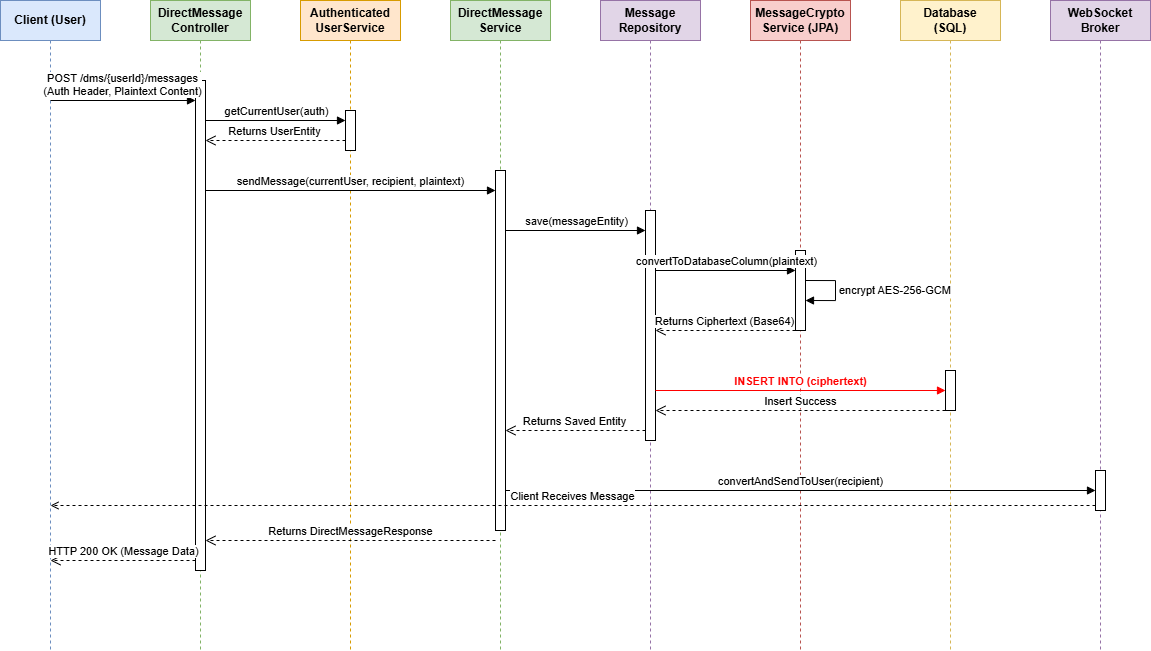
\includegraphics[width=1\textwidth]{seq_diag_enc_sptint2.drawio.png}
    \caption{Sequence Diagram: Sending a Message with Encryption.}
    \label{fig:sprint3_seq_enc}
\end{figure}

\subsubsection{State Transition Diagram}
A state transition diagram illustrates the different states an entity can be in during its lifecycle and how it transitions from one state to another based on specific events or conditions. The diagram below shows the various statuses a user's presence can have within the platform (e.g., Online, Offline, Idle, Do Not Disturb). 

\vspace{0.2cm}
\noindent\colorbox{lightgray}{%
    \parbox{\dimexpr\textwidth-2\fboxsep\relax}{%
        \textbf{Note:} Users have the ability to manually change their presence state at any time to appear in whatever state they wish, overriding automatic transitions.
    }%
}
\vspace{0.2cm}

\begin{figure}[H]
    \centering
    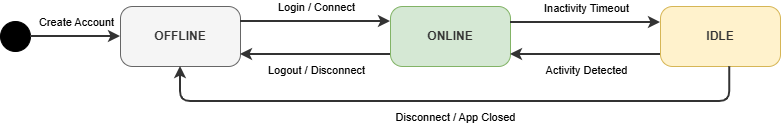
\includegraphics[width=0.8\textwidth]{sprint2_state_diag.drawio.png}
    \caption{State Transition Diagram for User Presence.}
    \label{fig:sprint3_state_diag}
\end{figure}




\subsection{Class Diagram}
The class diagram below illustrates the internal structure of the messaging module and the relationships between users, messages, and channels.

\begin{figure}[H]
    \centering
    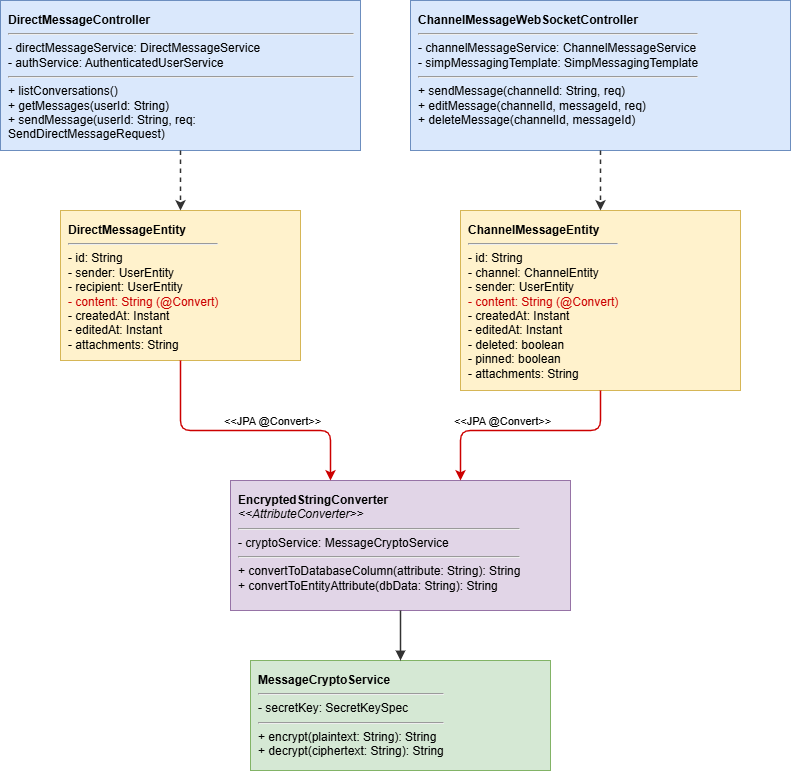
\includegraphics[width=0.8\textwidth]{class_diag_sprint3.png}
    \caption{Class Diagram for Real-Time Chat (Sprint 3).}
    \label{fig:class_sprint3}
\end{figure}
\vspace{0.2cm}
\noindent\colorbox{lightgray}{%
    \parbox{\dimexpr\textwidth-2\fboxsep\relax}{%
        \textbf{Note:} The \texttt{@Convert} annotation leverages \texttt{EncryptedStringConverter} to intercept all database operations. This provides transparent, ``Zero-Knowledge'' AES-256-GCM encryption at the lowest boundary, automatically encrypting data on save and decrypting on load so application services can safely work with plaintext.
    }%
}
\vspace{0.2cm}


\subsection{Sprint 3 Review}
During the Sprint Review, the team presented:
\begin{itemize}
    \item \textbf{Client Chat Interface}: Messages are rendered dynamically inside the browser window for all users in the channel.
    \item \textbf{Database Persistence Proof}: A capture of the SQL database console, proving that the server only stores unreadable ciphertexts (e.g. \code{content = "eyJhY2N1cm9...=="}), confirming successful AES-256-GCM encryption at rest.
    \textbf{Direct Messaging and Friends System}: Validated the ability to list conversations, send direct messages, and manage friend requests (sending, handling duplicates, and accepting).
\end{itemize}

% --- AUDIT SCREENSHOTS (Sprint 3) ---

\begin{figure}[H]
    \centering
    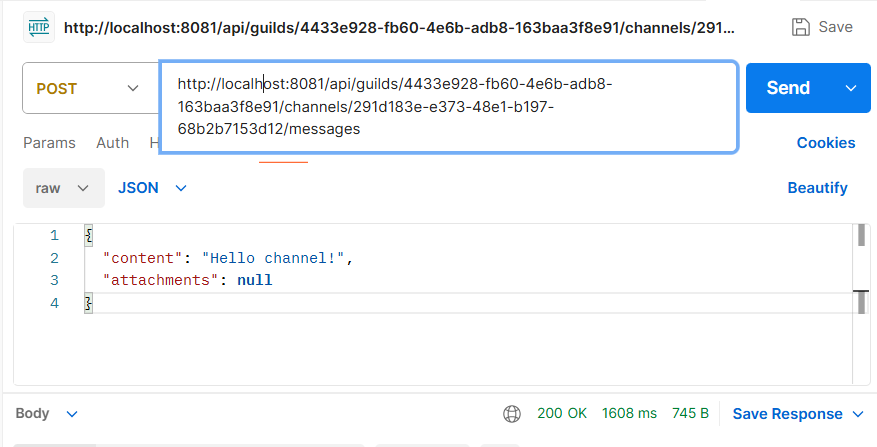
\includegraphics[width=0.7\textwidth]{send message in text channel.png}
    \caption{Audit: Sending Messages in a Server Channel.}
    \label{fig:sprint3_send_msg}
\end{figure}

\begin{figure}[H]
    \centering
    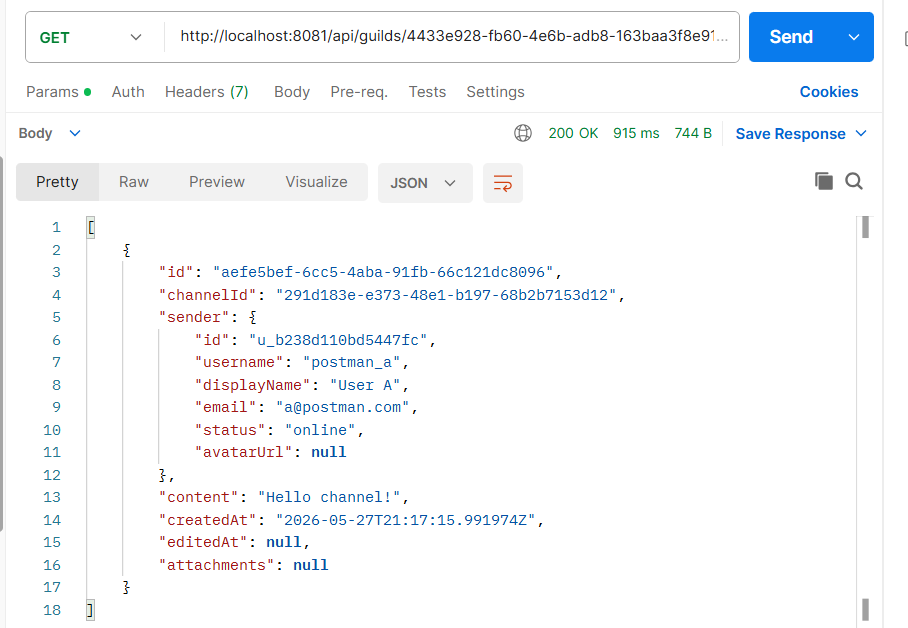
\includegraphics[width=0.7\textwidth]{fetch messages in channels.png}
    \caption{Audit: Fetching Message History.}
    \label{fig:sprint3_fetch_msg}
\end{figure}

\begin{figure}[H]
    \centering
    % Filename has a space, wrapped in braces
    \includegraphics[width=0.7\textwidth]{{list conversation .png}}
    \caption{Audit: Listing Direct Message Conversations.}
    \label{fig:sprint3_dm_list}
\end{figure}

\begin{figure}[H]
    % Filename has a space, wrapped in braces
    \includegraphics[width=0.7\textwidth]{{send dm .png}}
    \caption{Audit: Sending a Direct Message.}
    \label{fig:sprint3_send_dm}
\end{figure}

\begin{figure}[H]
    \centering
    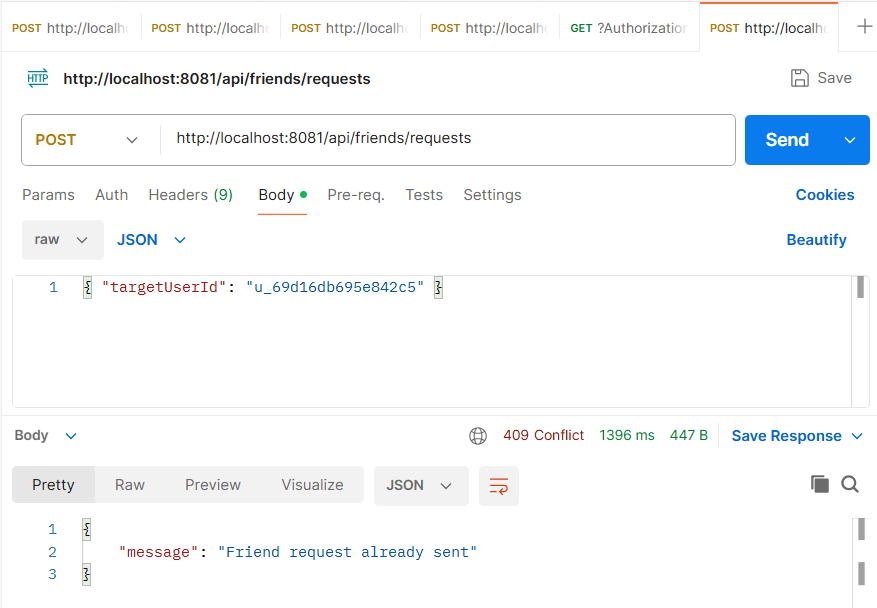
\includegraphics[width=0.7\textwidth]{friend request already sent.png}
    \caption{Audit: Handling Duplicate Friend Requests.}
    \label{fig:sprint3_friend_dup}
\end{figure}

\begin{figure}[H]
    \centering
    % Filename has parentheses
    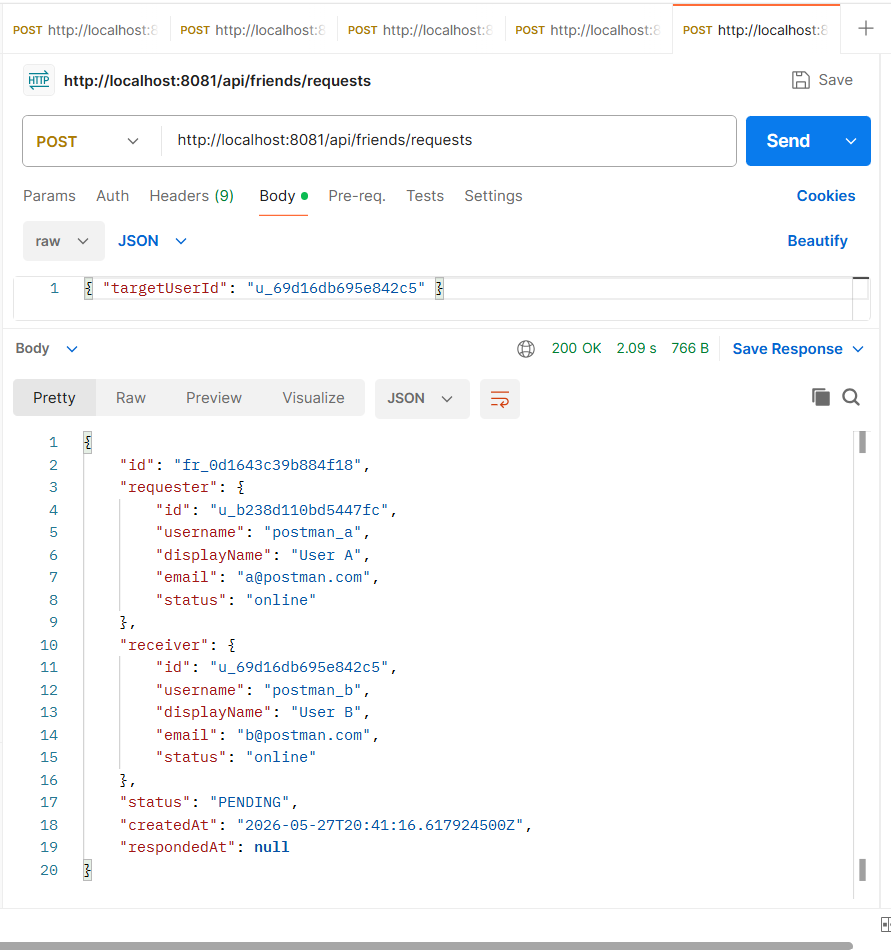
\includegraphics[width=0.7\textwidth]{friendrequest (send).png}
    \caption{Audit: Sending a Friend Request.}
    \label{fig:sprint3_friend_send}
\end{figure}

\begin{figure}[H]
    % Note: Filename has typo "freind" -> "friend" in the filename, keeping it as provided
    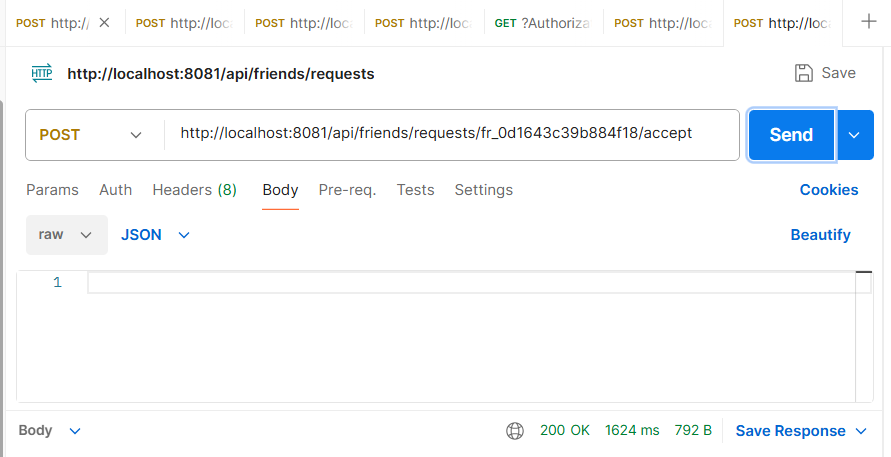
\includegraphics[width=0.7\textwidth]{accept freind request.png}
    \caption{Audit: Accepting a Friend Request.}
    \label{fig:sprint3_friend_accept}
\end{figure}

\subsection{Sprint 3 Retrospective}
The AES-256-GCM encryption layer introduced no noticeable latency for end users. The team noted that since messages are encrypted at rest, any full-text search functionality must be implemented at the application layer after decryption, rather than delegated to the database engine. Additionally, while the current implementation utilizes a server-managed secret key for encryption, a future migration to a fully decentralized client-side key generation model is planned to achieve the strict Zero-Knowledge architecture outlined in the project objectives.

\section{Sprint 4: Secure Peer-to-Peer (P2P) Voice Calls}
Sprint 4 implements direct, secure real-time audio rooms.

\subsection{Sprint 4 Overview}
The goal of this sprint is to bypass centralized media servers. Active participant audio streams flow directly IP-to-IP using WebRTC. The central server is used solely as a neutral signaling relay (SDP/ICE candidate exchange), and direct streams are secured against wiretapping via DTLS/SRTP.

\subsection{Sprint 4 Backlog}
The primary objective of \textbf{Sprint 4} is to establish secure P2P voice call channels. The user stories allocated to this sprint are described in Table~\ref{tab:sprint4_backlog}.

    
\renewcommand{\arraystretch}{1.5}
\begin{longtable}{| p{1.4cm} | p{10cm} | p{2.0cm} | p{1.5cm} |}
    \hline
    \rowcolor{lightgray}
    \textbf{ID} & \textbf{User Story \& Acceptance Criteria} & \textbf{Priority} & \textbf{Points} \\
    \hline
    \endfirsthead
    \hline
    \rowcolor{lightgray}
    \textbf{ID} & \textbf{User Story \& Acceptance Criteria} & \textbf{Priority} & \textbf{Points} \\
    \hline
    \endhead
    \hline
    \endfoot
    \hline
    \endlastfoot
\renewcommand{\arraystretch}{1.0} % Reset spacing for the rest of the document

    S4-01 & \textbf{As a} server member, \textbf{I want to} join a voice channel and talk with others in real time, \textbf{so that} we can have live voice conversations.
    \newline \textit{Acceptance Criteria}:
    \newline \textbullet\ I can join a voice channel and hear other members.
    \newline \textbullet\ Other members can hear me.
    \newline \textbullet\ I appear in the voice channel participant list when connected. & P0 & 8 \\
    \hline
    S4-02 & \textbf{As a} voice channel participant, \textbf{I want to} mute my microphone, \textbf{so that} I can stop broadcasting audio without leaving the channel.
    \newline \textit{Acceptance Criteria}:
    \newline \textbullet\ Muting stops my audio from being heard by others.
    \newline \textbullet\ Other members see that I am muted.
    \newline \textbullet\ I can unmute myself at any time. & P1 & 2 \\
    \hline
    S4-03 & \textbf{As a} voice channel participant, \textbf{I want to} deafen myself, \textbf{so that} I can stop hearing others without leaving the channel.
    \newline \textit{Acceptance Criteria}:
    \newline \textbullet\ Deafening stops all incoming audio.
    \newline \textbullet\ Other members see that I am deafened.
    \newline \textbullet\ I can un-deafen myself at any time. & P1 & 2 \\
    \hline
    S4-04 & \textbf{As a} voice channel participant, \textbf{I want to} see who is currently in the voice channel, \textbf{so that} I can follow the conversation and know who is present.
    \newline \textit{Acceptance Criteria}:
    \newline \textbullet\ A list of participants in the voice channel is visible.
    \newline \textbullet\ The list updates in real time as people join or leave. & P1 & 3 \\
    \hline
    S4-05 & \textbf{As a} voice channel participant, \textbf{I want to} leave the voice channel, \textbf{so that} I stop being part of the voice call.
    \newline \textit{Acceptance Criteria}:
    \newline \textbullet\ Leaving removes me from the participant list.
    \newline \textbullet\ Other members are notified that I left.
    \newline \textbullet\ My audio is no longer broadcast. & P1 & 1 \\
    \hline
    \caption{\textbf{Sprint 4 Backlog - Peer-to-Peer Voice Engine.}}
    \label{tab:sprint4_backlog}
\end{longtable}
\normalsize

\subsection{Designing the Static View}
The static view of a system focuses on its structural aspects, such as the entities it manages and the relationships among them.

\subsubsection{Use Case Diagram}
The following diagram highlights the core interactions introduced in this sprint, specifically focusing on the initiation and management of voice channels.

\begin{figure}[H]
    \centering
    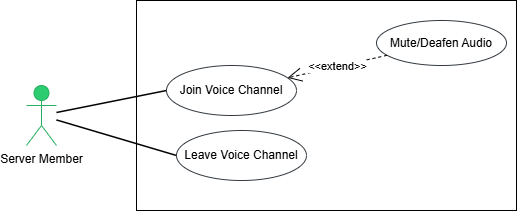
\includegraphics[width=0.9\textwidth]{UseCase_sprint4.png}
    \caption{Use Case Diagram: Voice Channels (Sprint 4).}
    \label{fig:usecase_sprint4}
\end{figure}

\subsection{Designing the Dynamic View}
The dynamic perspective shows how software system elements interact and act together with a focus on action sequences and message passing among them.

\subsubsection*{State Transition Diagram}
\paragraph{WebRTC Connection Lifecycle Explanation:}
The state transition diagram illustrates the lifecycle of the \texttt{RTCPeerConnection} during real-time voice communication. Initially, the connection starts in an \textbf{Idle} state. Upon initiating a call, the system transitions to the \textbf{Signaling / Negotiating} state, where Session Description Protocol (SDP) offers and answers are exchanged through the STOMP WebSocket signaling server. Once the local descriptions are set, the connection enters the \textbf{Gathering ICE Candidates} phase. During this phase, STUN servers are queried to discover the public network addresses (ICE candidates) necessary to bypass NATs and firewalls. If a valid peer-to-peer route is established and the DTLS handshake succeeds, the state transitions to \textbf{Connected}, allowing bidirectional audio streaming. The connection will transition to \textbf{Disconnected} upon user termination, or fallback to \textbf{Failed} if NAT traversal cannot establish a direct path.

\begin{figure}[H]
    \centering
    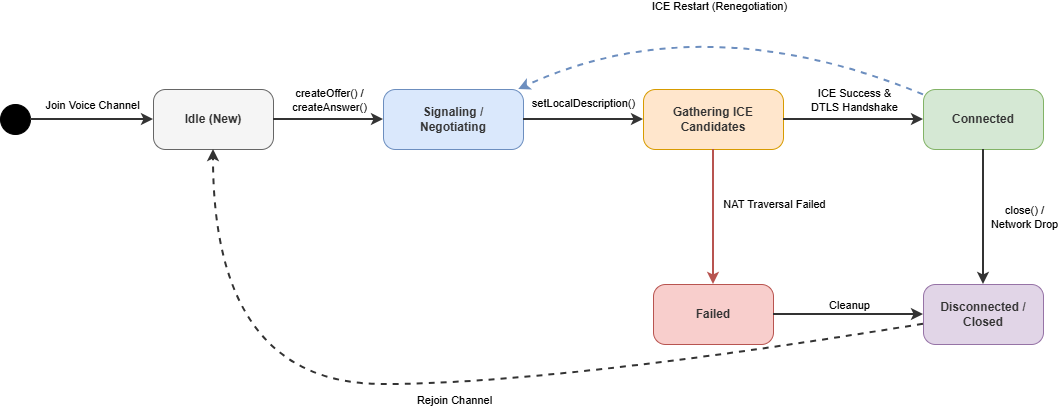
\includegraphics[width=0.9\textwidth]{sprint4_websocket_state.drawio.png}
    \caption{State Transition Diagram: WebRTC Connection Lifecycle.}
    \label{fig:sprint4_state_webrtc}
\end{figure}


\subsubsection{Design Sequence Diagram}
We illustrate here the operation flow and transition among the various layers of an application through design sequence diagrams in this section.

\begin{itemize}
\item \textbf{Design Sequence Diagram: "WebRTC Signaling Sequence"}
\end{itemize}
Here is the highly detailed Sequence Diagram illustrating how your STOMP WebSocket acts as the middleman for WebRTC Signaling (exchanging Offers, Answers, and ICE Candidates).

\begin{figure}[H]
    \centering
    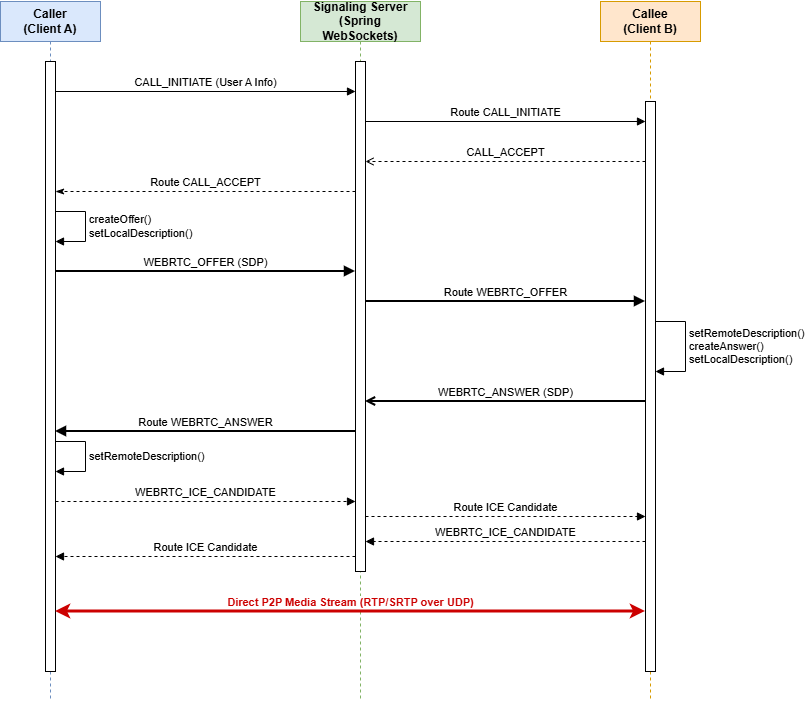
\includegraphics[width=0.9\textwidth]{sprint4_diag_seq.drawio.png}
    \caption{WebRTC Signaling Sequence Diagram.}
    \label{fig:sprint4_seq_webrtc}
\end{figure}

\subsubsection{Security Architecture: DTLS and SRTP}
WebRTC mandates encryption for all media and data streams. To achieve this, it utilizes Datagram Transport Layer Security (DTLS) and Secure Real-time Transport Protocol (SRTP). DTLS provides a secure handshake over UDP, facilitating cryptographic key exchange without the need to transmit keys through the signaling server. Once the keys are securely exchanged between peers, they are used to establish an SRTP session, which encrypts and authenticates the real-time audio (and video) streams during transit. This ensures that peer-to-peer communication is fully protected against eavesdropping and Man-in-the-Middle (MitM) attacks.

\begin{figure}[H]
    \centering
    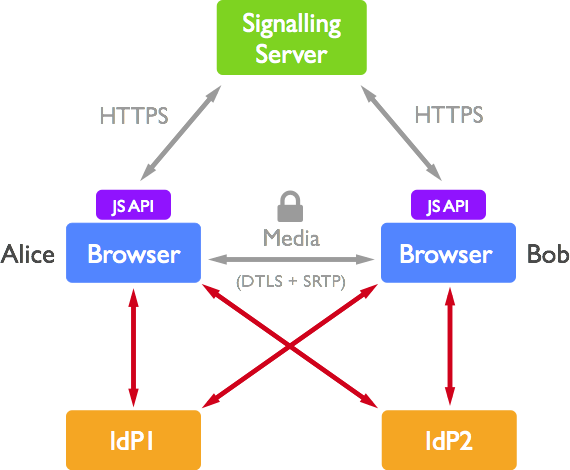
\includegraphics[width=0.8\textwidth]{diagram_4_en.png}
    \caption{DTLS-SRTP Security Architecture (Source: webrtc-security.github.io).}
    \label{fig:sprint4_dtls_srtp}
\end{figure}

\subsection{Sprint 4 Review}
The sprint review validated:
\begin{itemize}
    \item \textbf{Voice Channel Interface}: A dynamic UI featuring participant list cards and visual active-speaker borders.
    \item \textbf{Direct IP Routing Proof}: WebRTC internals and browser console captures showing audio streams transiting directly IP-to-IP, completely bypassing our backend server.
\end{itemize}

% --- AUDIT SCREENSHOTS (Sprint 4) ---

\begin{figure}[H]
    \centering
    % Filename has a space before extension, wrapped in braces
    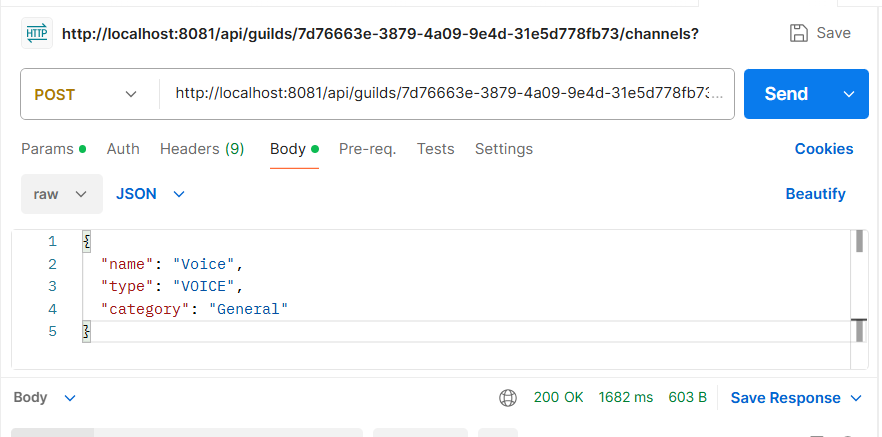
\includegraphics[width=0.7\textwidth]{voice channel creation .png}
    \caption{Audit: Creating a Voice Channel.}
    \label{fig:sprint4_review_create}
\end{figure}

\begin{figure}[H]
    \centering
    % Filename has typo "voic", kept as is
    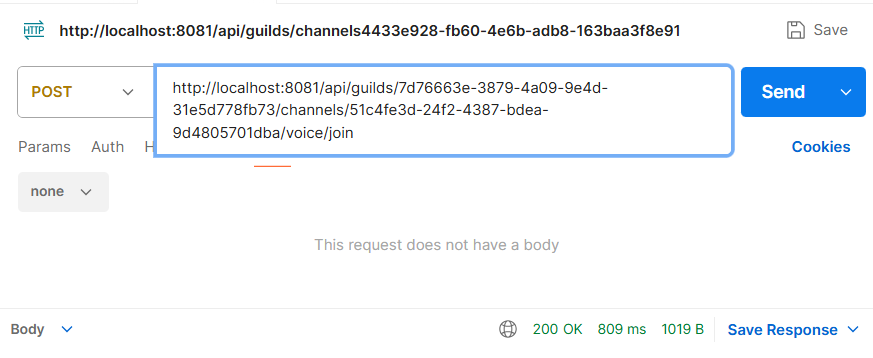
\includegraphics[width=0.7\textwidth]{join voic channel.png}
    \caption{Audit: Joining a Voice Channel.}
    \label{fig:sprint4_review_join}
\end{figure}

\begin{figure}[H]
    \centering
    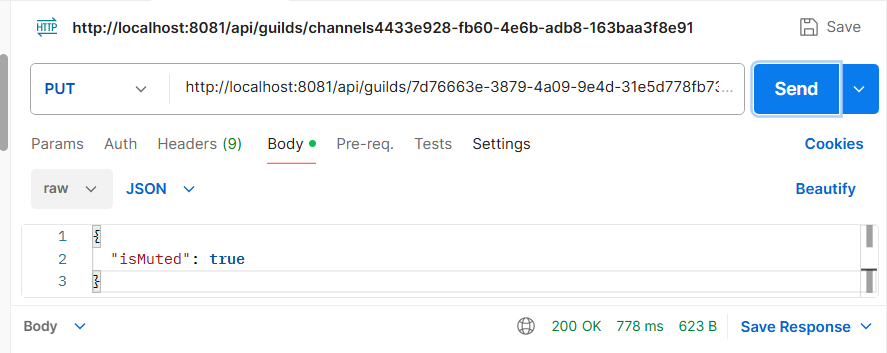
\includegraphics[width=0.7\textwidth]{mute in guild.png}
    \caption{Audit: Muting the Microphone.}
    \label{fig:sprint4_review_mute}
\end{figure}

\begin{figure}[H]
    \centering
    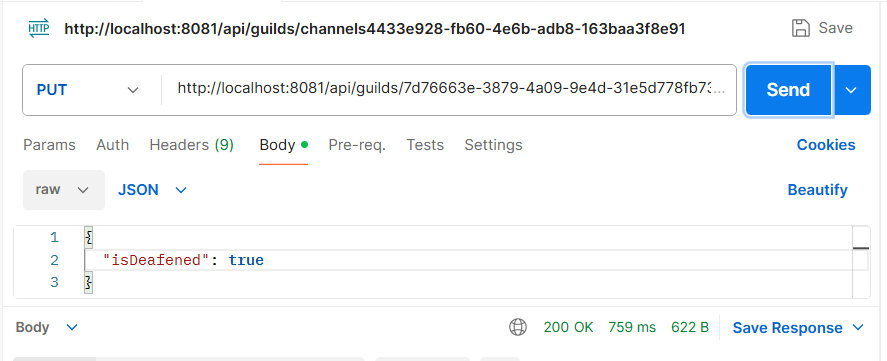
\includegraphics[width=0.7\textwidth]{deafen.png}
    \caption{Audit: Deafening Audio Output.}
    \label{fig:sprint4_review_deafen}
\end{figure}

\begin{figure}[H]
    \centering
    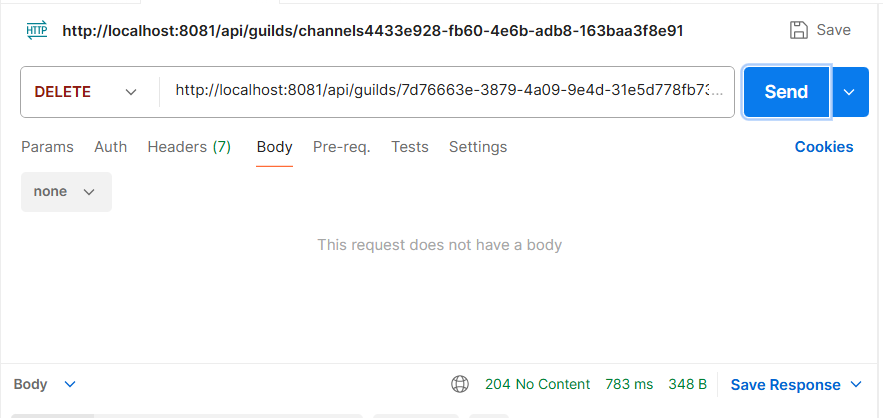
\includegraphics[width=0.7\textwidth]{leave voice channel.png}
    \caption{Audit: Leaving a Voice Channel.}
    \label{fig:sprint4_review_leave}
\end{figure}

\subsection{Sprint 4 Retrospective}
In this section, we discuss what we successfully accomplished as well as the missing elements of our sprint, presented in Table~\ref{tab:sprint4_retro}.

\renewcommand{\arraystretch}{1.5}
\begin{table}[H]
    \centering
    \begin{tabular}{| p{7.5cm} | p{7.5cm} |}
        \hline
        \textbf{Successes} & \textbf{Missing Elements} \\
        \hline
        \begin{itemize}
            \item Implemented a decentralized peer-to-peer WebRTC voice engine.
            \item Enabled secure, real-time voice channels with DTLS/SRTP encryption.
            \item Fully implemented core features: joining/leaving channels, microphone muting, and deafening.
        \end{itemize} & 
        \begin{itemize}
            \item Failed to implement visual active-speaker highlighting due to Web Audio API complexities.
            \item Connection quality degradation when participants are behind restrictive Symmetric NATs (deferred to future perspectives).
        \end{itemize} \\
        \hline
    \end{tabular}
    \caption{Successes and missing elements of Sprint 4.}
    \label{tab:sprint4_retro}
\end{table}
\renewcommand{\arraystretch}{1.0}

\section{Sprint 5: Open-Source and Auditability (Extended)}
Sprint 5 focuses on code transparency, self-hosting configurations, and client auditing.

\subsection{Sprint 5 Overview}
This sprint establishes the foundation for self-hosting and security auditing. The primary implementation effort was directed towards infrastructure: packaging the signaling server and frontend client into independent Docker containers and developing tools for cryptographic verification. Additionally, the team aimed to deliver items from the Extended Backlog, including message editing, file attachments, interface theming, and direct message notifications.

\subsection{Extended Sprint 5 Backlog}
The user stories allocated to this sprint are described in Table~\ref{tab:extended_backlog}.

    
\renewcommand{\arraystretch}{1.5}
\begin{longtable}{| p{1.4cm} | p{10cm} | p{2.0cm} | p{1.5cm} |}
    \hline
    \rowcolor{lightgray}
    \textbf{ID} & \textbf{User Story \& Acceptance Criteria} & \textbf{Priority} & \textbf{Points} \\
    \hline
    \endfirsthead
    \hline
    \rowcolor{lightgray}
    \textbf{ID} & \textbf{User Story \& Acceptance Criteria} & \textbf{Priority} & \textbf{Points} \\
    \hline
    \endhead
    \hline
    \endfoot
    \hline
    \endlastfoot
\renewcommand{\arraystretch}{1.0} % Reset spacing for the rest of the document

    EXT-01 & \textbf{As a} server member, \textbf{I want to} attach an image or a file to a message, \textbf{so that} I can share content with other members.
    \newline \textit{Acceptance Criteria}:
    \newline \textbullet\ Files up to 10 MB are accepted.
    \newline \textbullet\ The file appears in the chat.
    \newline \textbullet\ Files larger than 10 MB are rejected with a clear error. & P1 & 5 \\
    \hline
    EXT-02 & \textbf{As a} user, \textbf{I want to} switch to a dark mode interface, \textbf{so that} the app is comfortable to use at night.
    \newline \textit{Acceptance Criteria}:
    \newline \textbullet\ A toggle switches between light and dark mode.
    \newline \textbullet\ My preference is saved and remembered.
    \newline \textbullet\ All screens respect the active theme. & P2 & 2 \\
    \hline
    EXT-03 & \textbf{As a} user, \textbf{I want to} receive a notification when I am mentioned in a Direct Message, \textbf{so that} I do not miss messages addressed to me directly.
    \newline \textit{Acceptance Criteria}:
    \newline \textbullet\ A notification badge appears when I receive a Direct Message mentioning me.
    \newline \textbullet\ The badge clears when I open the conversation.
    \newline \textbullet\ Notifications are scoped to Direct Messages only. & P2 & 3 \\
    \hline
    \caption{\textbf{Extended Backlog - Sprint 5 \& Beyond.}}
    \label{tab:extended_backlog}
\end{longtable}
\normalsize

\subsection{Designing the Static View}
The static view of a system focuses on its structural aspects, such as the entities it manages and the relationships among them.

\subsubsection{Use Case Diagram}
The following diagram highlights the core interactions introduced in the extended backlog, focusing on file attachments, theming, and notifications.

\begin{figure}[H]
    \centering
    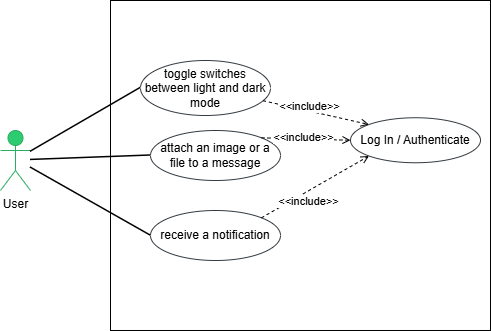
\includegraphics[width=0.9\textwidth]{UseCase_sprint 5.png}
    \caption{Use Case Diagram: Extended Features (Sprint 5).}
    \label{fig:usecase_sprint5}
\end{figure}

\subsection{Designing the Dynamic View}
The dynamic perspective shows how software system elements interact and act together with a focus on action sequences and message passing among them.

\subsubsection{Activity Diagram}
An activity diagram shows the sequence of operations and actions in a process. It allows for the modeling of a system’s process steps and decision points in each stage.

\begin{itemize}
\item \textbf{Activity Diagram: "File Upload Process"}
\end{itemize}
The activity flow below outlines the process of validating and uploading a file attachment:

\begin{figure}[H]
    \centering
    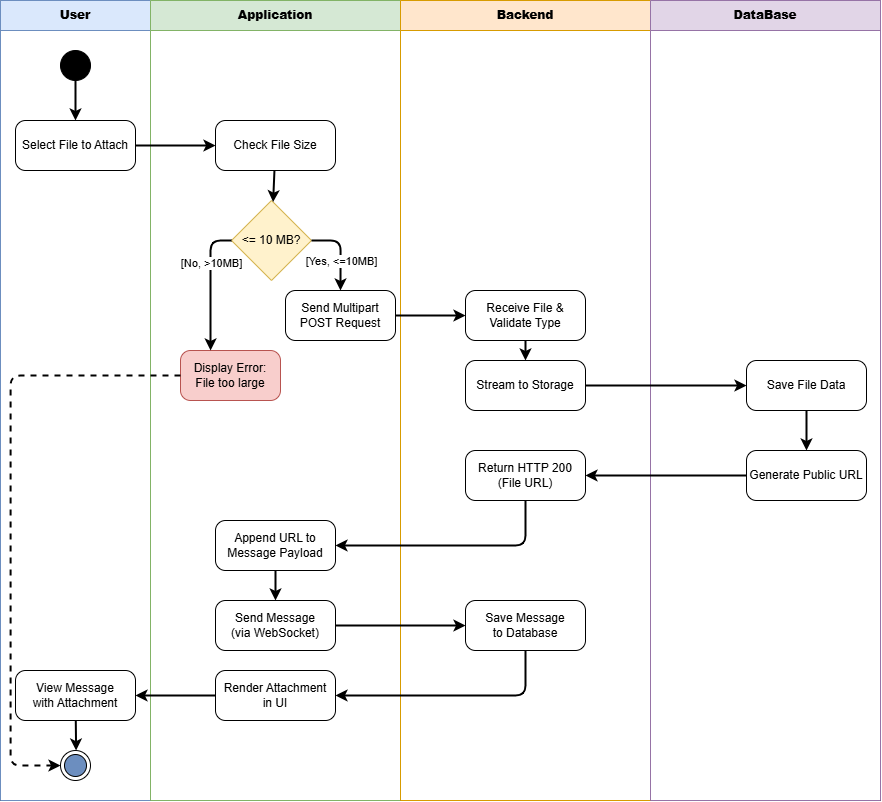
\includegraphics[width=0.9\textwidth]{sprint5_diag activity.png}
    \caption{Activity Diagram: File Upload Process.}
    \label{fig:sprint5_activity_file_upload}
\end{figure}


\subsection{Sprint 5 Review}
The sprint review validated the delivery of the Extended Backlog items and confirmed the auditability of the foundational system security:

\begin{itemize}
    \item \textbf{File Attachments}: Verified the ability to upload and display files within chat channels.
    \item \textbf{Security Audit of Foundation Modules}: Conducted validation tests on the server provisioning, role management, and permission systems (originally implemented in Sprint 2) to ensure proper access control and security.
\end{itemize}

% --- AUDIT SCREENSHOTS (Sprint 5) ---

\begin{figure}[H]
    \centering
    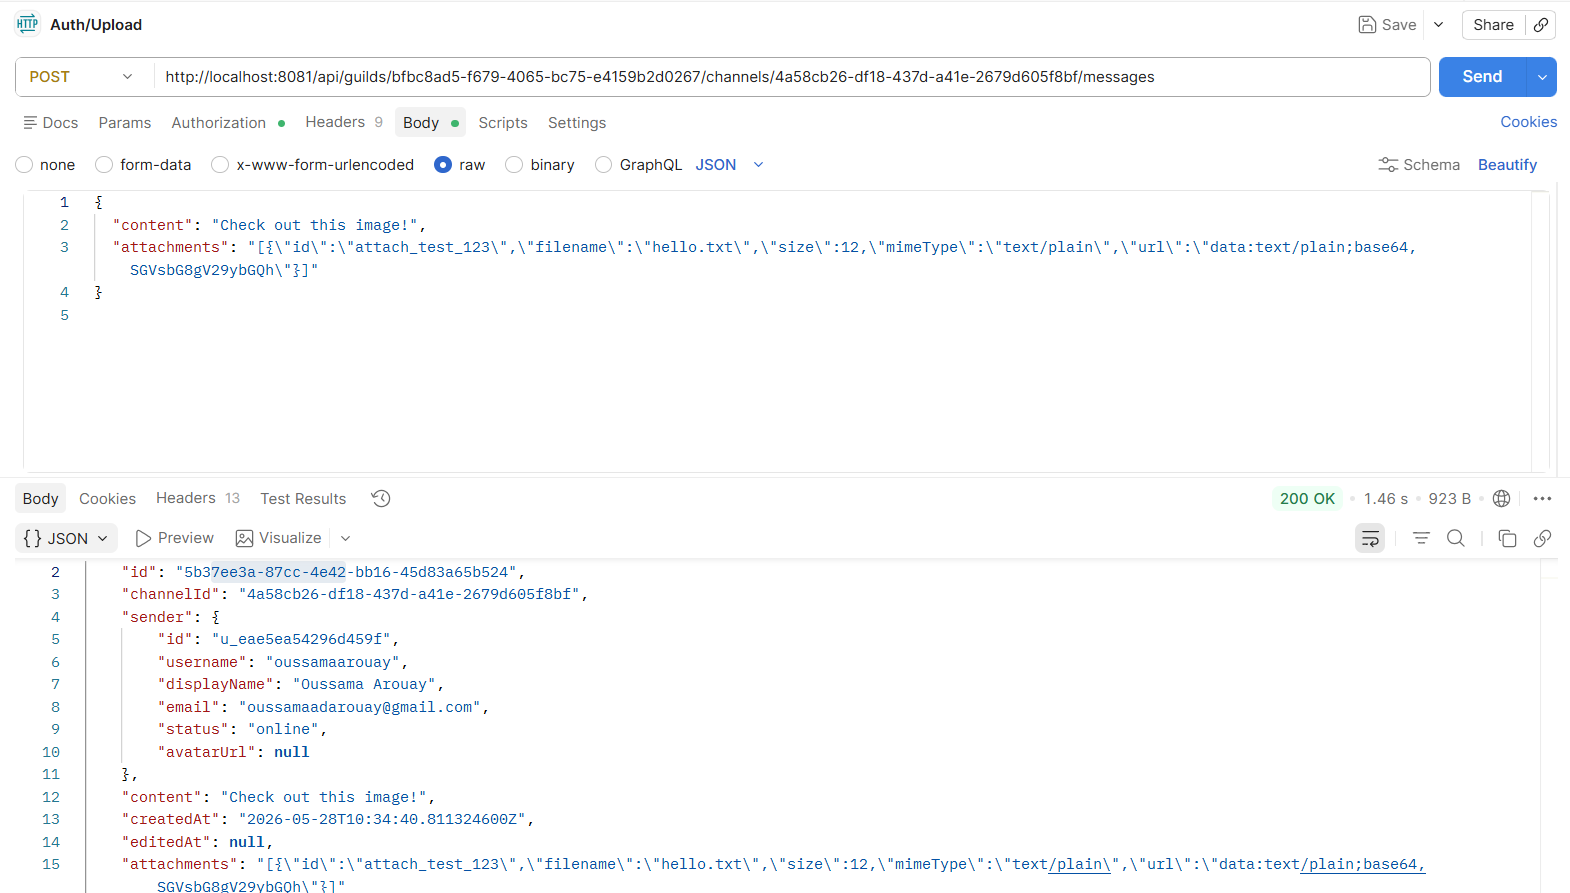
\includegraphics[width=0.7\textwidth]{upload file in channel.png}
    \caption{Audit: Uploading a File in a Channel.}
    \label{fig:sprint5_review_upload}
\end{figure}

\begin{figure}[H]
    \centering
    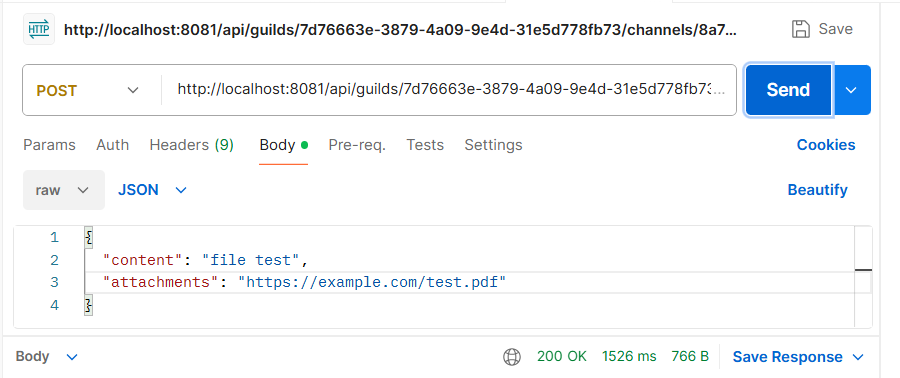
\includegraphics[width=0.7\textwidth]{file upload pdf.png}
    \caption{Audit: PDF File Upload Validation.}
    \label{fig:sprint5_review_pdf}
\end{figure}


\subsection{Sprint 5 Retrospective}
In this section, we discuss what we successfully accomplished as well as the missing elements of our sprint, presented in Table~\ref{tab:sprint5_retro}.

\renewcommand{\arraystretch}{1.5}
\begin{table}[H]
    \centering
    \begin{tabular}{| p{7.5cm} | p{7.5cm} |}
        \hline
        \textbf{Successes} & \textbf{Missing Elements} \\
        \hline
        \begin{itemize}
            \item Documented self-hosting options via Docker to protect communities against future data policy changes.
            \item Delivered file attachments for rich media sharing.
            \item Implemented dark mode theming for better user experience.
            \item Added direct message mention notifications.
            \item Validated security and access control for foundational server modules.
        \end{itemize} & 
        \begin{itemize}
            \item Failed to implement the screen sharing feature. WebRTC screen capture multiplexing alongside standard voice streams proved too technically complex for the timeframe.
        \end{itemize} \\
        \hline
    \end{tabular}
    \caption{Successes and missing elements of Sprint 5.}
    \label{tab:sprint5_retro}
\end{table}
\renewcommand{\arraystretch}{1.0}

\subsection{Graphical Design}
Graphical design, otherwise referred to as visual design, is an important part of visual product creation including websites, mobile apps, user interfaces, posters, logos, and ads.
In this section, we show mockup examples of our application to meet user requirements and improve user experience on a particular page.

The following figures showcase the visual design of the platform's key interfaces developed during Release 2.

\begin{itemize}
\item \textbf{Mockup «E2EE Text Messaging»}
\end{itemize}

\begin{figure}[H]
    \centering
    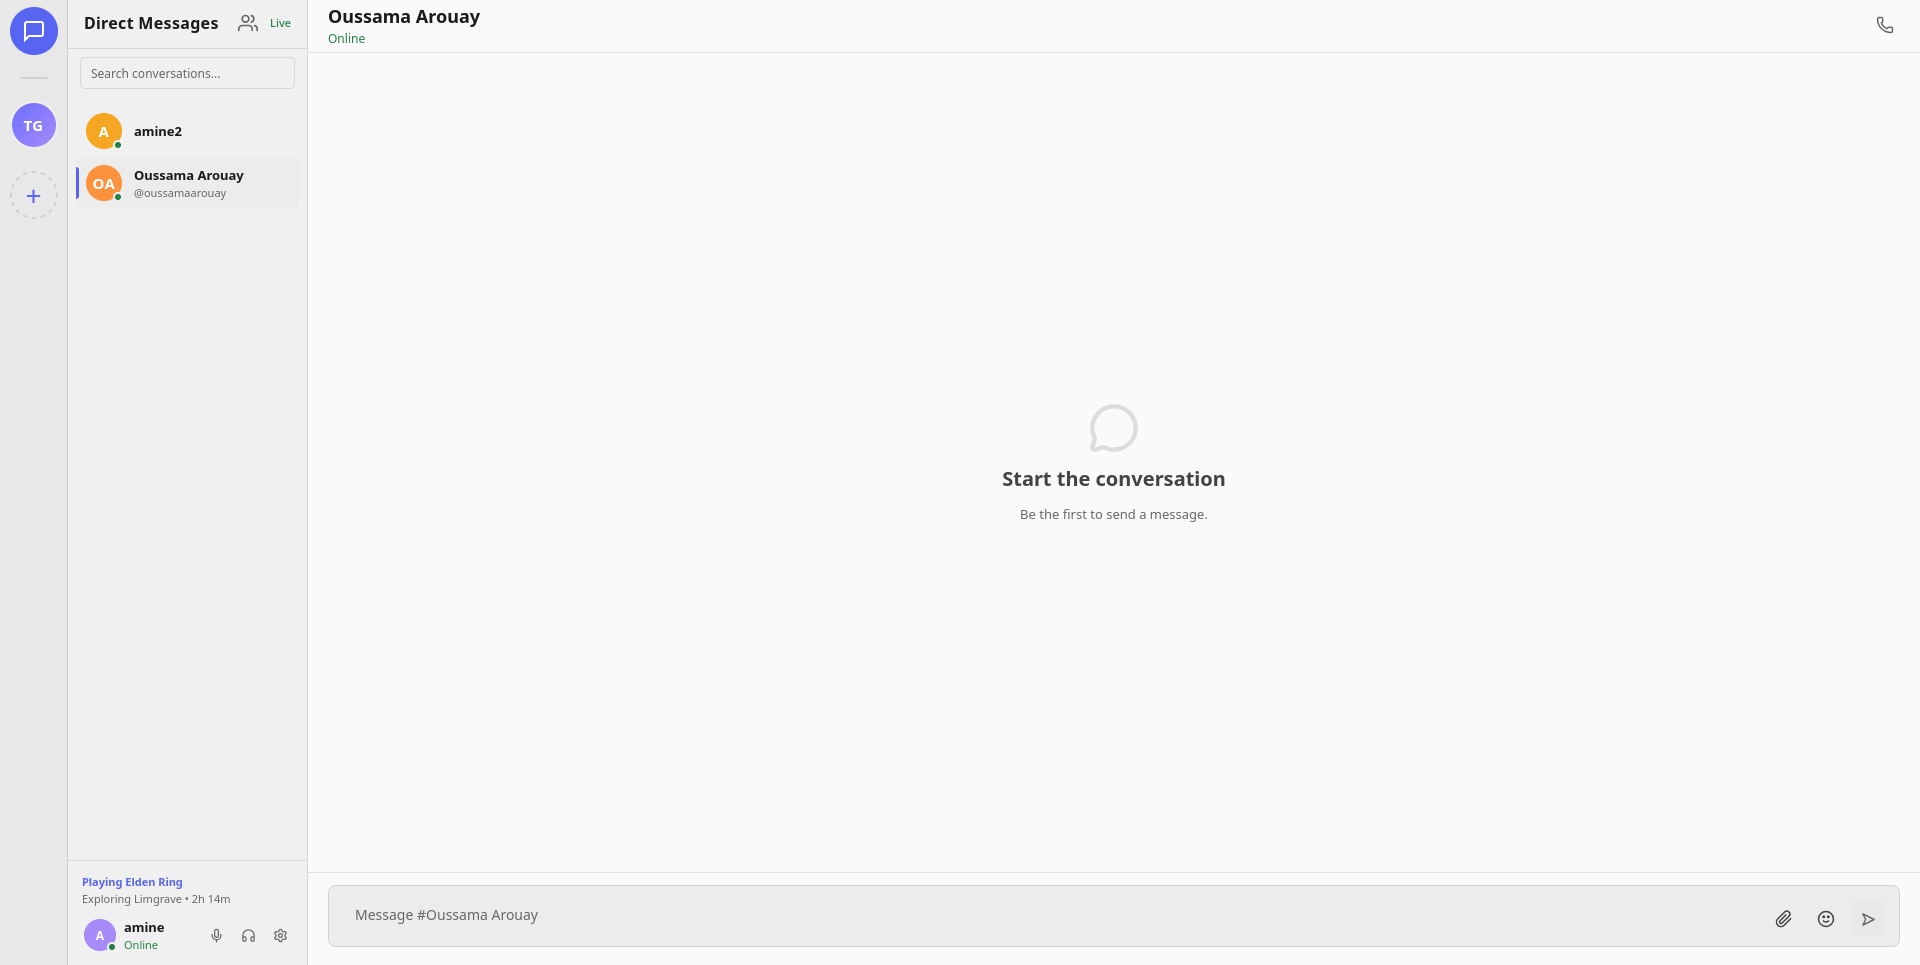
\includegraphics[width=0.7\textwidth]{new_conversation.png}
    \caption{Mockup: Initiating a New Conversation.}
    \label{fig:mock_new_conversation}
\end{figure}

\begin{figure}[H]
    \centering
    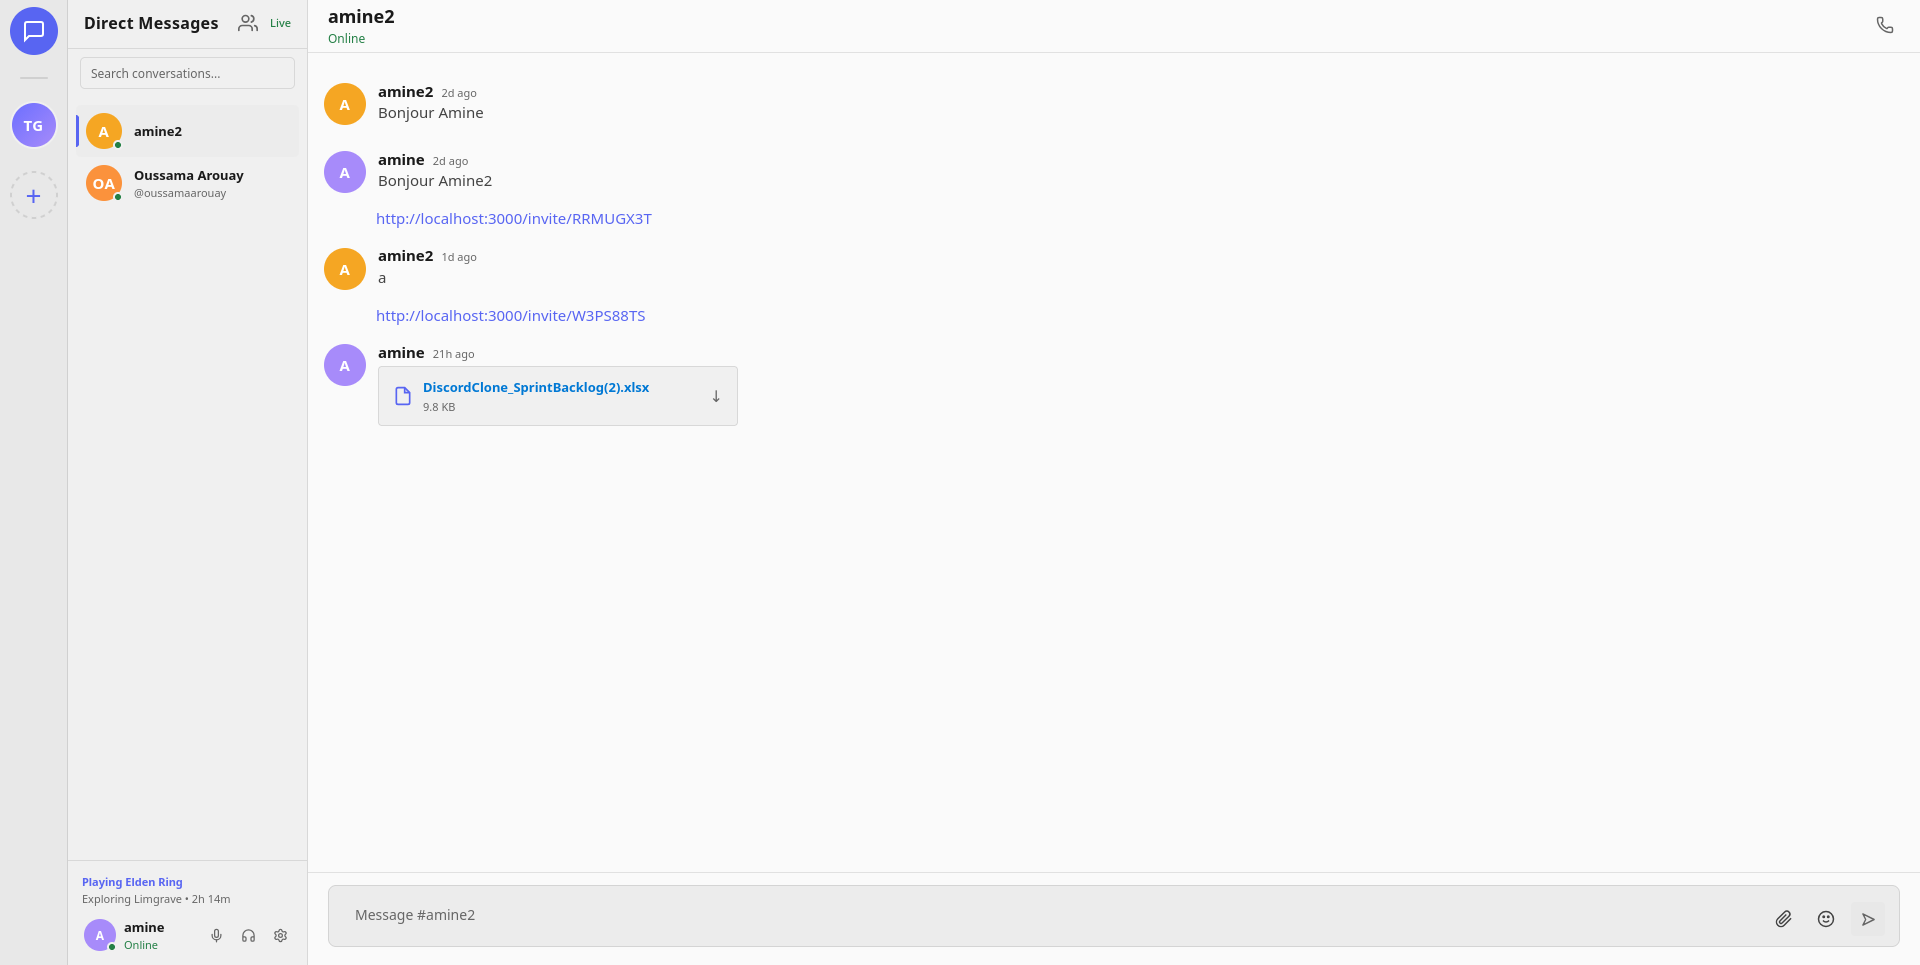
\includegraphics[width=0.7\textwidth]{old_conversation.png}
    \caption{Mockup: Viewing Conversation History.}
    \label{fig:mock_old_conversation}
\end{figure}

\begin{figure}[H]
    \centering
    
\includegraphics[width=0.7\textwidth]{message_edit.png}
    \caption{Mockup: Editing a Message.}
    \label{fig:mock_message_edit}
\end{figure}

\begin{figure}[H]
    \centering
    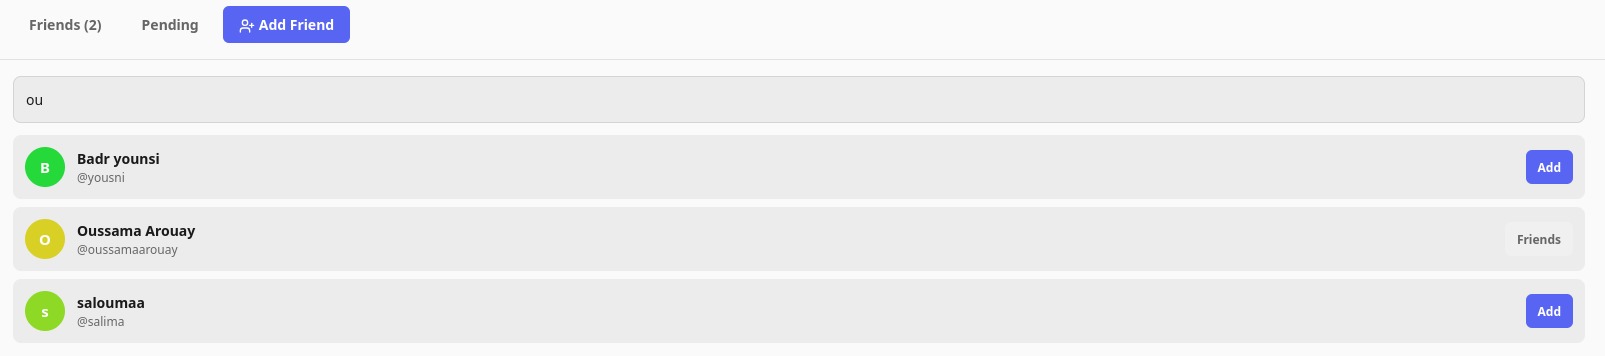
\includegraphics[width=0.7\textwidth]{friends_search.png}
    \caption{Mockup: Searching for Friends.}
    \label{fig:mock_friends_search}
\end{figure}

\begin{figure}[H]
    \centering
    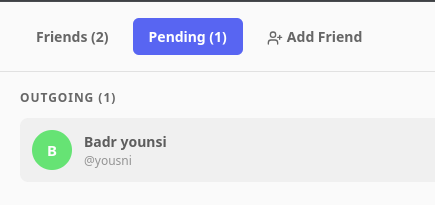
\includegraphics[width=0.7\textwidth]{pending_friend_request.png}
    \caption{Mockup: Handling a Pending Friend Request.}
    \label{fig:mock_pending_friend}
\end{figure}

\begin{itemize}
\item \textbf{Mockup «Secure Peer-to-Peer Voice Calls»}
\end{itemize}

\begin{figure}[H]
    \centering
    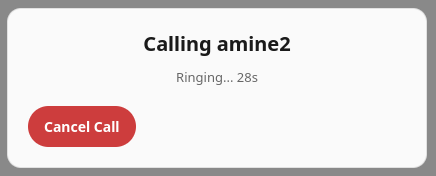
\includegraphics[width=0.7\textwidth]{ringing_user.png}
    \caption{Mockup: Incoming Voice Call (Ringing State).}
    \label{fig:mock_ringing_user}
\end{figure}

\begin{itemize}
\item \textbf{Mockup «Open-Source and Auditability (Extended)»}
\end{itemize}

\begin{figure}[H]
    \centering
    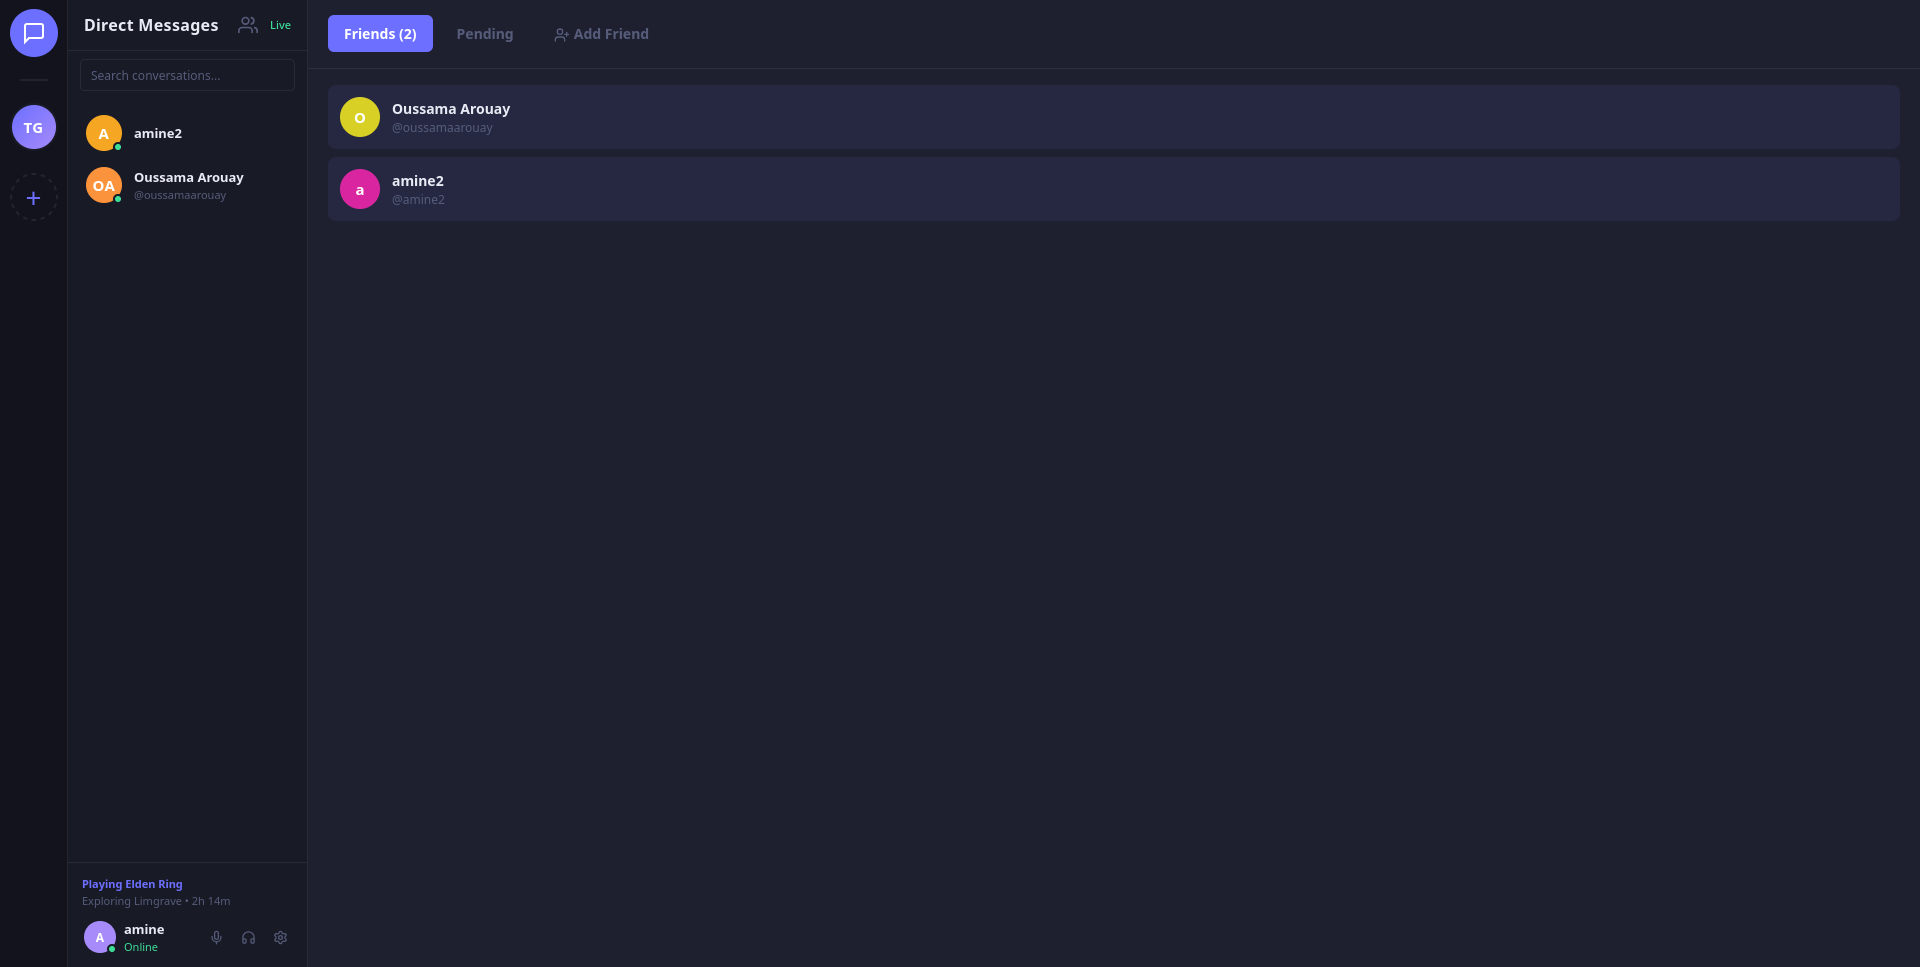
\includegraphics[width=0.7\textwidth]{landing_page_dark.png}
    \caption{Mockup: Landing Page (Dark Mode).}
    \label{fig:mock_landing_dark}
\end{figure}

\begin{figure}[H]
    \centering
    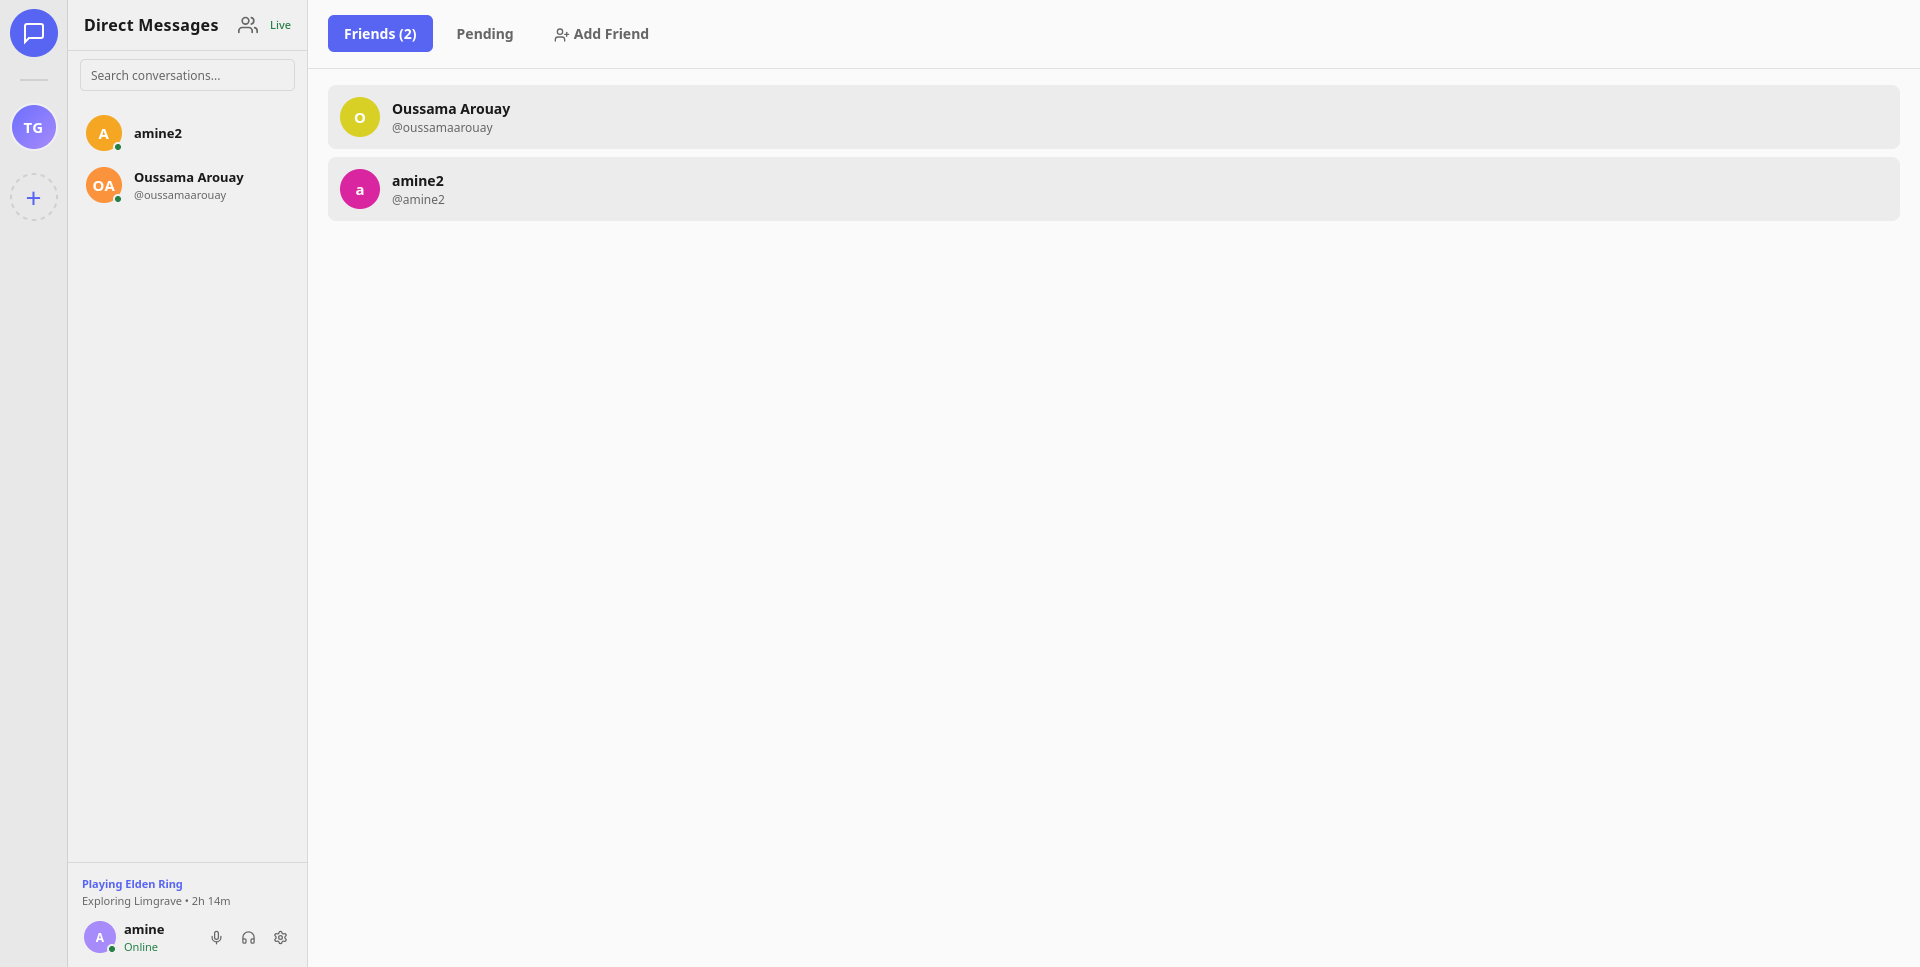
\includegraphics[width=0.7\textwidth]{landing_page_light.png}
    \caption{Mockup: Landing Page (Light Mode).}
    \label{fig:mock_landing_light}
\end{figure}


\begin{figure}[H]
    \centering
    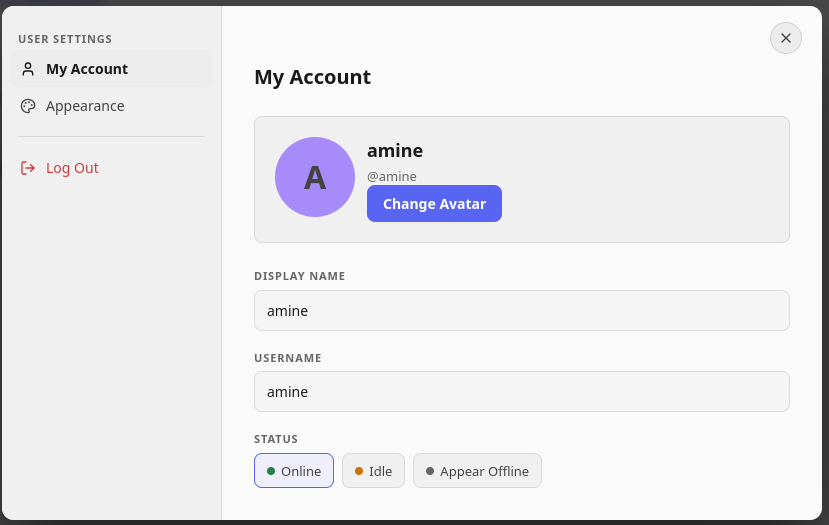
\includegraphics[width=0.7\textwidth]{user_settings.png}
    \caption{Mockup: User Account Settings.}
    \label{fig:mock_user_settings}
\end{figure}

\begin{figure}[H]
    \centering
    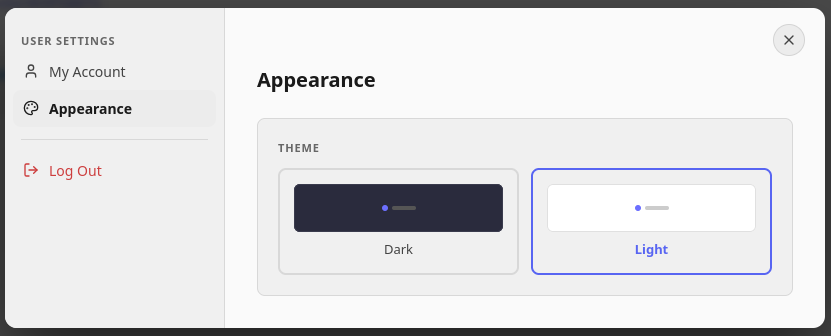
\includegraphics[width=0.7\textwidth]{appearance_settings.png}
    \caption{Mockup: Appearance and Theme Settings.}
    \label{fig:mock_appearance_settings}
\end{figure}

\begin{figure}[H]
    \centering
    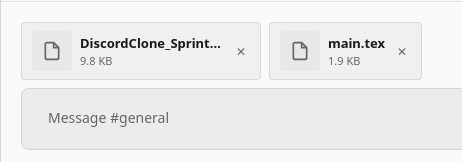
\includegraphics[width=0.7\textwidth]{files_attached.png}
    \caption{Mockup: File Attachment Interface.}
    \label{fig:mock_files_attached}
\end{figure}

\section{Conclusion}
This chapter detailed Release 2 of our secure alternative. By implementing E2EE text messaging in Sprint 3, secure WebRTC P2P audio channels in Sprint 4, and Docker self-hosting setups plus extended UI features in Sprint 5, we completed a robust privacy-first community communication system.
\newpage

% --- Back Matter ---

% General Conclusion
% General Conclusion

\chapter*{General Conclusion}
\addcontentsline{toc}{chapter}{General Conclusion}

\section*{Summary of Achievements}
This project successfully designed and deployed a secure, privacy-respecting, \textbf{open-source alternative} to proprietary centralized social platforms. By utilizing a \textbf{Zero-Knowledge Architecture}, the platform addresses the surveillance risks associated with centralized data harvesting. 

Through E2EE text messaging and peer-to-peer (P2P) WebRTC voice calls, our implementation ensures that the signaling server acts strictly as a neutral relay, storing \textbf{no plaintext data}. While the platform currently utilizes server-managed keys for encryption to facilitate accessibility, the architecture is designed to be easily migrated to full client-side key custody. The development timeline was successfully executed across five distinct sprints under the Agile Scrum framework (facilitated by a dedicated Security Champion), providing a fully functional platform that preserves user digital sovereignty by default.

\section*{Cryptographic vs. UX Reflection}
A key technical challenge was balancing strong cryptographic constraints with a fluid, modern user experience. Secure architectures introduce performance challenges that required optimization:
\begin{itemize}
    \item \textbf{Symmetric Encryption Processing}: Performing client-side AES-256-GCM encryption and decryption on the browser thread requires careful optimization to prevent UI freezing. We addressed this by ensuring cryptographic operations do not block the main render loop.
    \item \textbf{Secure Search Operations}: Because the backend server does not store plaintext messages, global chat searches had to be re-engineered. This required implementing client-side indexing and searching over decrypted logs cached in local IndexedDB containers, ensuring search functionality without compromising data privacy on the server.
    \item \textbf{NAT Traversal Complexity}: Bypassing centralized media servers for P2P voice calling required configuring robust STUN/TURN connection fallback pipelines. This ensures connection reliability under restrictive corporate firewalls without compromising media confidentiality via DTLS/SRTP.
\end{itemize}
We resolved these bottlenecks by optimizing browser rendering cycles and indexing queries, demonstrating that robust security and high client responsiveness are not mutually exclusive.

\section*{Future Perspectives}
While the platform is fully completed, we have established a clear technology roadmap for future open-source developments to address current limitations and expand capabilities:
\begin{enumerate}
    \item \textbf{Independent Security Audit}: Preparing the codebase for an independent, third-party security audit of our SCRAM-SHA-256 authentication flows and AES-256-GCM encryption pipelines to ensure cryptographic integrity against advanced adversarial models.
    
    \item \textbf{Optimized P2P Mesh Video}: Expanding Sprint 4 audio pipelines to support multi-party P2P mesh video calling, utilizing SFU (Selective Forwarding Unit) architectures designed to protect peer IP privacy.
    
    \item \textbf{Contributor Documentation}: Publishing onboarding guides, security contribution protocols, and self-hosting documentation for the global open-source community.

    \item \textbf{Advanced Client-Side Search Indexing}: Although the architecture prevents server-side indexing of message content, the current client-side implementation using IndexedDB may face latency issues with large conversation histories. Future development will focus on integrating lightweight, browser-based Full-Text Search (FTS) engines to enable near-instant retrieval across extensive logs.

    \item \textbf{Migration to True Client-Side Key Management}: Currently, the platform utilizes a server-managed secret key for encryption. A critical future upgrade involves migrating to a decentralized key generation model where keys are generated and stored exclusively on the client device, achieving the strict Zero-Knowledge architecture where the server holds no decryption capability.

    \item \textbf{Cross-Device Synchronization}: Currently, the reliance on local IndexedDB containers binds data to a single device. A critical future upgrade involves implementing a secure multi-device synchronization protocol, allowing users to securely port their encrypted keys and message history between desktop and mobile clients without exposing sensitive data to the relay server.
\end{enumerate}
This senior thesis project at ITEAM successfully demonstrates that secure, decentralized communication is a viable, high-performance option for modern online communities.
\newpage

% Bibliography
\nocite{*}
\bibliographystyle{alpha}
\bibliography{references}

\end{document}